% Capitolul 15: Recapitulare și susținerea proiectelor
% Analiza avansată a seriilor de timp și previziune -- Programul de master Statistică aplicată și data science, anul I, semestrul 2, Academia de Studii Economice din București
% GENERAT de latex/build_chapter15.py -- modificați generatorul, nu acest fișier.

\newcommand{\coursename}{Analiza avansată a seriilor de timp și previziune}
\def\atslang{ro}
% Preambul comun ATS -- Analiza avansată a seriilor de timp și previziune / Advanced Time Series Analysis and Forecasting
% (Beamer, 16:9). Același design ca MFM, SFM și TSA (copiat din TSA, 5 octombrie 2026). Înainte de % Preambul comun ATS -- Analiza avansată a seriilor de timp și previziune / Advanced Time Series Analysis and Forecasting
% (Beamer, 16:9). Același design ca MFM, SFM și TSA (copiat din TSA, 5 octombrie 2026). Înainte de % Preambul comun ATS -- Analiza avansată a seriilor de timp și previziune / Advanced Time Series Analysis and Forecasting
% (Beamer, 16:9). Același design ca MFM, SFM și TSA (copiat din TSA, 5 octombrie 2026). Înainte de \input{../../latex/preamble} se definește
%   \newcommand{\coursename}{Advanced Time Series Analysis and Forecasting}          (EN)
%   \newcommand{\coursename}{Analiza avansată a seriilor de timp și previziune}       (RO)  și  \def\atslang{ro}
% Fișierele .tex se află în EN/Courses, EN/Seminars, RO/Cursuri, RO/Seminarii (două niveluri sub rădăcină).
% Deck-urile sînt generate de latex/build_chapterN.py / build_seminarN.py (vezi latex/ats_build.py).

\documentclass[9pt, aspectratio=169, t]{beamer}
\providecommand{\coursename}{Advanced Time Series Analysis and Forecasting}

% Ensure content fits on slides
\setbeamersize{text margin left=8mm, text margin right=8mm}
% Smaller institute font (title page)
\setbeamerfont{institute}{size=\footnotesize}

%=============================================================================
% THEME AND STYLE CONFIGURATION
%=============================================================================
\usetheme{default}
% Using default theme for clean header/footer control

% Color Palette (matching Redispatch PDF)
\definecolor{MainBlue}{RGB}{26, 58, 110}
\definecolor{AccentBlue}{RGB}{26, 58, 110}
\definecolor{IDAred}{RGB}{205, 0, 0}
\definecolor{DarkGray}{RGB}{51, 51, 51}
\definecolor{MediumGray}{RGB}{128, 128, 128}
\definecolor{LightGray}{RGB}{248, 248, 248}
\definecolor{VeryLightGray}{RGB}{235, 235, 235}
\definecolor{KeynoteGray}{RGB}{218, 218, 218}
\definecolor{SectionGray}{RGB}{120, 120, 120}
\definecolor{FooterGray}{RGB}{100, 100, 100}
\definecolor{Crimson}{RGB}{220, 53, 69}
\definecolor{Forest}{RGB}{46, 125, 50}
\definecolor{Amber}{RGB}{181, 133, 63}
\definecolor{Orange}{RGB}{230, 126, 34}
\definecolor{Purple}{RGB}{142, 68, 173}

% Gradient background (exact Keynote 315° gradient: white to RGB 218,218,218)
\setbeamertemplate{background}{%
    \begin{tikzpicture}[remember picture, overlay]
        \shade[shading=axis, shading angle=315,
        top color=white, bottom color=KeynoteGray]
        (current page.south west) rectangle (current page.north east);
    \end{tikzpicture}%
}
% Fallback solid color for compatibility
\setbeamercolor{background canvas}{bg=}

\setbeamercolor{palette primary}{bg=MainBlue, fg=white}
\setbeamercolor{palette secondary}{bg=MainBlue!85, fg=white}
\setbeamercolor{palette tertiary}{bg=MainBlue!70, fg=white}
\setbeamercolor{structure}{fg=MainBlue}
\setbeamercolor{title}{fg=IDAred}
\setbeamercolor{frametitle}{fg=IDAred, bg=}
\setbeamercolor{block title}{bg=MainBlue, fg=white}
\setbeamercolor{block body}{bg=VeryLightGray, fg=DarkGray}
\setbeamercolor{block title alerted}{bg=Crimson, fg=white}
\setbeamercolor{block body alerted}{bg=Crimson!8, fg=DarkGray}
\setbeamercolor{block title example}{bg=Forest, fg=white}
\setbeamercolor{block body example}{bg=Forest!8, fg=DarkGray}
\setbeamercolor{item}{fg=MainBlue}

% Footer colors (override Madrid theme blue)
\setbeamercolor{author in head/foot}{fg=FooterGray, bg=}
\setbeamercolor{title in head/foot}{fg=FooterGray, bg=}
\setbeamercolor{date in head/foot}{fg=FooterGray, bg=}
\setbeamercolor{section in head/foot}{fg=FooterGray, bg=}
\setbeamercolor{subsection in head/foot}{fg=FooterGray, bg=}

% Bullet styles (apply everywhere including blocks)
\setbeamertemplate{itemize item}{\color{MainBlue}$\boxdot$}
\setbeamertemplate{itemize subitem}{\color{MainBlue}$\blacktriangleright$}
\setbeamertemplate{itemize subsubitem}{\color{MainBlue}\tiny$\bullet$}
\setbeamertemplate{itemize/enumerate body begin}{\normalsize}
\setbeamertemplate{itemize/enumerate subbody begin}{\normalsize}

% Item spacing - compact style
\setlength{\leftmargini}{10pt}       % Level 1: minimal indent
\setlength{\leftmarginii}{10pt}      % Level 2: minimal additional indent
% Compact list spacing (zero extra space before/after lists in blocks)
\makeatletter
\def\@listi{\leftmargin\leftmargini \topsep 0pt \parsep 0pt \itemsep 0pt}
\def\@listii{\leftmargin\leftmarginii \topsep 0pt \parsep 0pt \itemsep 0pt}
\makeatother

\setbeamertemplate{navigation symbols}{}

%=============================================================================
% CUSTOM HEADLINE
%=============================================================================
\setbeamertemplate{headline}{%
    \vskip10pt%
    \hbox to \paperwidth{%
        \hskip0.5cm%
        {\small\color{FooterGray}\renewcommand{\hyperlink}[2]{##2}\insertsectionhead}%
        \hfill%
        \textcolor{FooterGray}{\small\insertframenumber}%
        \hskip0.5cm%
    }%
    \vskip4pt%
    {\color{FooterGray}\hrule height 0.4pt}%
}

%=============================================================================
% CUSTOM FOOTER
%=============================================================================
\usepackage{fontawesome5}

\setbeamertemplate{footline}{%
    {\color{FooterGray}\hrule height 0.4pt}%
    \vskip4pt%
    \hbox to \paperwidth{%
        \hskip0.5cm%
        \textcolor{FooterGray}{\small\coursename}%
        \hfill%
        \raisebox{-0.1em}{%
            \begin{tikzpicture}[x=0.08em, y=0.08em, line width=0.4pt]
                \draw[FooterGray] (0,3) -- (1,4) -- (2,3.5) -- (3,5) -- (4,4) -- (5,6) -- (6,5.5) -- (7,4) -- (8,5) -- (9,7) -- (10,6) -- (11,5) -- (12,6.5) -- (13,8) -- (14,7) -- (15,6) -- (16,7.5) -- (17,9) -- (18,8) -- (19,7) -- (20,8.5) -- (21,10) -- (22,9) -- (23,8) -- (24,9.5);
            \end{tikzpicture}%
        }%
        \hskip0.5cm%
    }%
    \vskip6pt%
}

%=============================================================================
% PACKAGES
%=============================================================================
\usepackage[utf8]{inputenc}
\DeclareUnicodeCharacter{03B1}{\ensuremath{\alpha}}
\usepackage[T1]{fontenc}
\usepackage{amsmath, amssymb, amsthm}
\usepackage{mathtools}
\usepackage{bm}
\usepackage{tikz}
\usetikzlibrary{arrows.meta, positioning, shapes, calc, decorations.pathreplacing, shadings}
\usepackage{booktabs}
\usepackage{multirow}
\usepackage{array}
\usepackage{graphicx}
\usepackage{animate}
\usepackage{hyperref}
\usepackage{colortbl}
\usepackage{listings}
\lstset{language=Python, basicstyle=\ttfamily\scriptsize, keywordstyle=\color{MainBlue}\bfseries,
  commentstyle=\color{Forest}, stringstyle=\color{Crimson}, breaklines=true,
  frame=none, backgroundcolor=\color{VeryLightGray}, xleftmargin=2mm}
\hypersetup{colorlinks=true, linkcolor=MainBlue, urlcolor=MainBlue}
\graphicspath{{../../logos/}{../../charts/}{../../photos/}}
\usepackage{xcolor}
\hfuzz=2pt  % Suppress tiny overfull warnings (<2pt)
\vfuzz=2pt  % Suppress tiny vertical overfull warnings (<2pt)

%=============================================================================
% QUANTLET COMMANDS
%   \quantlet{<displayed name>}{<url>}       (generic)
%   \atsquantlet{Ch_05}{ATS_ch5_garch}       -> https://github.com/danpele/Advanced-Time-Series/tree/main/Quantlets/Ch_05/ATS_ch5_garch
%   \qlurl{<folder>} is defined per chapter by the generator (Quantlets/Ch_NN/<folder>)
%=============================================================================
\newcommand{\atsrepo}{https://github.com/danpele/Advanced-Time-Series}
\newcommand{\atsqlbase}{https://github.com/danpele/Advanced-Time-Series/tree/main/Quantlets}
\newcommand{\quantlet}[2]{%
    \hfill\href{#2}{%
        \raisebox{-0.15em}{
\includegraphics[height=0.7em]{ql_logo.png}}%
        \textcolor{MainBlue}{\tiny\ #1}%
    }%
}
\newcommand{\atsquantlet}[2]{\quantlet{\detokenize{#2}}{\atsqlbase/#1/#2}}

%=============================================================================
% NOTEBOOKS (Google Colab)
%   \colaburl{notebooks/EN/chapter5_seminar_notebook.ipynb} -> the Colab link of a file in the ATS repo
%   \nb: the chapter notebook (each seminar deck redefines it with \renewcommand)
%=============================================================================
\newcommand{\colaburl}[1]{https://colab.research.google.com/github/danpele/Advanced-Time-Series/blob/main/#1}
\newcommand{\nb}{https://colab.research.google.com/github/danpele/Advanced-Time-Series/tree/main/notebooks/EN}
\newcommand{\nbname}{notebooks/EN}

%=============================================================================
% SLIDE HELPERS (used by the generators; the same as in MFM)
%=============================================================================
% local font size for list bodies (the preamble forces \normalsize)
\newcommand{\itemsize}[1]{\setbeamertemplate{itemize/enumerate body begin}{#1}\setbeamertemplate{itemize/enumerate subbody begin}{#1}}
\newcommand{\intitle}[1]{{\hypersetup{urlcolor=white}#1}}   % white links inside coloured title bars
\newcommand{\imgcap}[1]{{\scriptsize #1}\\[0.5mm]}          % caption under a photo
\newcommand{\imgcredit}[2]{{\tiny\color{FooterGray}\href{#1}{#2}}}   % image credit: source URL, author/licence
\newcommand{\aiprompt}[1]{{\ttfamily\color{MainBlue}#1}}     % a prompt to an AI assistant

%=============================================================================
% SEMINARS: student version by default; the instructor wrapper *_solutions.tex sets \solutionstrue
%=============================================================================
\makeatletter\@ifundefined{ifsolutions}{\expandafter\newif\csname ifsolutions\endcsname}{}\makeatother
\newcommand{\solonly}[1]{\ifsolutions #1\fi}
\newcommand{\propsub}{\ifsolutions\else\framesubtitle{\ifdefined\atslang Rezolvarea se discută la seminar\else Solution discussed in class\fi}\fi}

%=============================================================================
% APPENDIX AND CHAPTER LINKS (latex/appendix_links.py writes the calls; it also re-declares these
% macros before \begin{document}, so the decks compile with or without this preamble block)
%=============================================================================
\providecommand{\atsapplink}[3]{\hypertarget{#2}{}\hyperlink{#1}{\beamergotobutton{#3}}}
\providecommand{\atsappback}[2]{\begin{tikzpicture}[remember picture,overlay]\node[anchor=south east] at ([xshift=-3mm,yshift=7mm]current page.south east){\hyperlink{#1}{\beamerreturnbutton{#2}}};\end{tikzpicture}}
\providecommand{\atschlink}[2]{\href{#1}{#2}}
\providecommand{\atschlinkt}[2]{\href{#1}{\usebeamercolor[fg]{frametitle}#2}}

%=============================================================================
% QUANTINAR COMMAND: link către un curs Quantinar (subiecte avansate)
%=============================================================================
\newcommand{\quantinar}[2]{%
    \href{#2}{%
        \raisebox{-0.15em}{
\includegraphics[height=0.8em]{qr_logo.png}}%
        \textcolor{MainBlue}{\scriptsize\ #1}%
    }%
}

%=============================================================================
% CUSTOM TITLE PAGE
%=============================================================================
\defbeamertemplate*{title page}{hybrid}[1][]
{
    \vspace{0.2cm}
    % Logos row - top header (with clickable links)
    \begin{center}
        \href{https://www.ase.ro}{
\includegraphics[height=1.0cm]{ase_logo.png}}\hspace{0.3cm}%
        \href{https://theida.net}{
\includegraphics[height=1.0cm]{ida_logo.png}}\hspace{0.3cm}%
        \href{https://blockchain-research-center.com}{
\includegraphics[height=1.0cm]{brc_logo.png}}\hspace{0.3cm}%
        \href{https://www.ai4efin.ase.ro}{
\includegraphics[height=1.0cm]{ai4efin_logo.png}}\hspace{0.3cm}%
        \href{https://ipe.ro/new}{
\includegraphics[height=1.0cm]{acad_logo.png}}\hspace{0.3cm}%
        \href{https://www.digital-finance-msca.com}{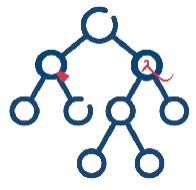
\includegraphics[height=1.0cm]{msca_logo.png}}%
    \end{center}

    \vspace{0.6cm}

    % Main title with Q logos on sides (with clickable links)
    \begin{center}
        \begin{minipage}{0.1\textwidth}
            \centering
            \href{https://quantlet.com}{
\includegraphics[height=1.1cm]{ql_logo.png}}
        \end{minipage}%
        \begin{minipage}{0.78\textwidth}
            \centering
            {\LARGE\bfseries\usebeamercolor[fg]{title}\inserttitle}

            \vspace{0.3cm}

            {\usebeamerfont{subtitle}\usebeamercolor[fg]{title}\insertsubtitle}
        \end{minipage}%
        \begin{minipage}{0.1\textwidth}
            \centering
            \href{https://quantinar.com}{
\includegraphics[height=1.1cm]{qr_logo.png}}
        \end{minipage}
    \end{center}

    \vspace{0.6cm}

    % Authors (left aligned)
    \hspace{0.5cm}{\usebeamerfont{author}\insertauthor}

    \vspace{0.3cm}

    % Institute/Affiliations (left aligned)
    \hspace{0.5cm}\begin{minipage}[t]{0.9\textwidth}
        \raggedright\small\insertinstitute
    \end{minipage}
}

%=============================================================================
% THEOREM ENVIRONMENTS
%=============================================================================
\theoremstyle{definition}
\setbeamertemplate{theorems}[numbered]
\ifdefined\atslang
\newtheorem{defn}{Definiție}
\newtheorem{thm}{Teoremă}
\newtheorem{prop}{Propoziție}
\newtheorem{rmk}{Observație}
\else
\newtheorem{defn}{Definition}
\newtheorem{thm}{Theorem}
\newtheorem{prop}{Proposition}
\newtheorem{rmk}{Remark}
\fi

%=============================================================================
% CENTRED MINIPAGE (no extra vertical space)
%=============================================================================
\newenvironment{cminipage}[1]{%
    \par\noindent\hfill\begin{minipage}{#1}\ignorespaces
}{%
    \end{minipage}\hfill\null\par
}

%=============================================================================
% CUSTOM COMMANDS
%=============================================================================
\newcommand{\E}{\mathbb{E}}
\newcommand{\Var}{\text{Var}}
\newcommand{\Cov}{\text{Cov}}
\newcommand{\Corr}{\text{Corr}}
\newcommand{\R}{\mathbb{R}}
\newcommand{\N}{\mathbb{N}}
\newcommand{\Z}{\mathbb{Z}}
\newcommand{\B}{\mathbf{B}}
\newcommand{\imark}{\textcolor{MainBlue}{\textbullet}}
\newcommand{\RMSE}{\text{RMSE}}
\newcommand{\MAE}{\text{MAE}}
\newcommand{\MAPE}{\text{MAPE}}

% Boldface vector/matrix commands (VAR, VECM, state space)
\newcommand{\bY}{\mathbf{Y}}
\newcommand{\bX}{\mathbf{X}}
\newcommand{\bA}{\mathbf{A}}
\newcommand{\bB}{\mathbf{B}}
\newcommand{\bepsilon}{\boldsymbol{\varepsilon}}
\newcommand{\bSigma}{\boldsymbol{\Sigma}}
\newcommand{\bPhi}{\boldsymbol{\Phi}}
\newcommand{\bGamma}{\boldsymbol{\Gamma}}
\newcommand{\bPi}{\boldsymbol{\Pi}}
\newcommand{\bc}{\mathbf{c}}
\newcommand{\balpha}{\boldsymbol{\alpha}}
\newcommand{\bbeta}{\boldsymbol{\beta}}
\newcommand{\bvarepsilon}{\boldsymbol{\varepsilon}}

% Seminar marks
\newcommand{\correct}{\textcolor{Forest}{\checkmark}}
\newcommand{\incorrect}{\textcolor{Crimson}{\texttimes}}
 se definește
%   \newcommand{\coursename}{Advanced Time Series Analysis and Forecasting}          (EN)
%   \newcommand{\coursename}{Analiza avansată a seriilor de timp și previziune}       (RO)  și  \def\atslang{ro}
% Fișierele .tex se află în EN/Courses, EN/Seminars, RO/Cursuri, RO/Seminarii (două niveluri sub rădăcină).
% Deck-urile sînt generate de latex/build_chapterN.py / build_seminarN.py (vezi latex/ats_build.py).

\documentclass[9pt, aspectratio=169, t]{beamer}
\providecommand{\coursename}{Advanced Time Series Analysis and Forecasting}

% Ensure content fits on slides
\setbeamersize{text margin left=8mm, text margin right=8mm}
% Smaller institute font (title page)
\setbeamerfont{institute}{size=\footnotesize}

%=============================================================================
% THEME AND STYLE CONFIGURATION
%=============================================================================
\usetheme{default}
% Using default theme for clean header/footer control

% Color Palette (matching Redispatch PDF)
\definecolor{MainBlue}{RGB}{26, 58, 110}
\definecolor{AccentBlue}{RGB}{26, 58, 110}
\definecolor{IDAred}{RGB}{205, 0, 0}
\definecolor{DarkGray}{RGB}{51, 51, 51}
\definecolor{MediumGray}{RGB}{128, 128, 128}
\definecolor{LightGray}{RGB}{248, 248, 248}
\definecolor{VeryLightGray}{RGB}{235, 235, 235}
\definecolor{KeynoteGray}{RGB}{218, 218, 218}
\definecolor{SectionGray}{RGB}{120, 120, 120}
\definecolor{FooterGray}{RGB}{100, 100, 100}
\definecolor{Crimson}{RGB}{220, 53, 69}
\definecolor{Forest}{RGB}{46, 125, 50}
\definecolor{Amber}{RGB}{181, 133, 63}
\definecolor{Orange}{RGB}{230, 126, 34}
\definecolor{Purple}{RGB}{142, 68, 173}

% Gradient background (exact Keynote 315° gradient: white to RGB 218,218,218)
\setbeamertemplate{background}{%
    \begin{tikzpicture}[remember picture, overlay]
        \shade[shading=axis, shading angle=315,
        top color=white, bottom color=KeynoteGray]
        (current page.south west) rectangle (current page.north east);
    \end{tikzpicture}%
}
% Fallback solid color for compatibility
\setbeamercolor{background canvas}{bg=}

\setbeamercolor{palette primary}{bg=MainBlue, fg=white}
\setbeamercolor{palette secondary}{bg=MainBlue!85, fg=white}
\setbeamercolor{palette tertiary}{bg=MainBlue!70, fg=white}
\setbeamercolor{structure}{fg=MainBlue}
\setbeamercolor{title}{fg=IDAred}
\setbeamercolor{frametitle}{fg=IDAred, bg=}
\setbeamercolor{block title}{bg=MainBlue, fg=white}
\setbeamercolor{block body}{bg=VeryLightGray, fg=DarkGray}
\setbeamercolor{block title alerted}{bg=Crimson, fg=white}
\setbeamercolor{block body alerted}{bg=Crimson!8, fg=DarkGray}
\setbeamercolor{block title example}{bg=Forest, fg=white}
\setbeamercolor{block body example}{bg=Forest!8, fg=DarkGray}
\setbeamercolor{item}{fg=MainBlue}

% Footer colors (override Madrid theme blue)
\setbeamercolor{author in head/foot}{fg=FooterGray, bg=}
\setbeamercolor{title in head/foot}{fg=FooterGray, bg=}
\setbeamercolor{date in head/foot}{fg=FooterGray, bg=}
\setbeamercolor{section in head/foot}{fg=FooterGray, bg=}
\setbeamercolor{subsection in head/foot}{fg=FooterGray, bg=}

% Bullet styles (apply everywhere including blocks)
\setbeamertemplate{itemize item}{\color{MainBlue}$\boxdot$}
\setbeamertemplate{itemize subitem}{\color{MainBlue}$\blacktriangleright$}
\setbeamertemplate{itemize subsubitem}{\color{MainBlue}\tiny$\bullet$}
\setbeamertemplate{itemize/enumerate body begin}{\normalsize}
\setbeamertemplate{itemize/enumerate subbody begin}{\normalsize}

% Item spacing - compact style
\setlength{\leftmargini}{10pt}       % Level 1: minimal indent
\setlength{\leftmarginii}{10pt}      % Level 2: minimal additional indent
% Compact list spacing (zero extra space before/after lists in blocks)
\makeatletter
\def\@listi{\leftmargin\leftmargini \topsep 0pt \parsep 0pt \itemsep 0pt}
\def\@listii{\leftmargin\leftmarginii \topsep 0pt \parsep 0pt \itemsep 0pt}
\makeatother

\setbeamertemplate{navigation symbols}{}

%=============================================================================
% CUSTOM HEADLINE
%=============================================================================
\setbeamertemplate{headline}{%
    \vskip10pt%
    \hbox to \paperwidth{%
        \hskip0.5cm%
        {\small\color{FooterGray}\renewcommand{\hyperlink}[2]{##2}\insertsectionhead}%
        \hfill%
        \textcolor{FooterGray}{\small\insertframenumber}%
        \hskip0.5cm%
    }%
    \vskip4pt%
    {\color{FooterGray}\hrule height 0.4pt}%
}

%=============================================================================
% CUSTOM FOOTER
%=============================================================================
\usepackage{fontawesome5}

\setbeamertemplate{footline}{%
    {\color{FooterGray}\hrule height 0.4pt}%
    \vskip4pt%
    \hbox to \paperwidth{%
        \hskip0.5cm%
        \textcolor{FooterGray}{\small\coursename}%
        \hfill%
        \raisebox{-0.1em}{%
            \begin{tikzpicture}[x=0.08em, y=0.08em, line width=0.4pt]
                \draw[FooterGray] (0,3) -- (1,4) -- (2,3.5) -- (3,5) -- (4,4) -- (5,6) -- (6,5.5) -- (7,4) -- (8,5) -- (9,7) -- (10,6) -- (11,5) -- (12,6.5) -- (13,8) -- (14,7) -- (15,6) -- (16,7.5) -- (17,9) -- (18,8) -- (19,7) -- (20,8.5) -- (21,10) -- (22,9) -- (23,8) -- (24,9.5);
            \end{tikzpicture}%
        }%
        \hskip0.5cm%
    }%
    \vskip6pt%
}

%=============================================================================
% PACKAGES
%=============================================================================
\usepackage[utf8]{inputenc}
\DeclareUnicodeCharacter{03B1}{\ensuremath{\alpha}}
\usepackage[T1]{fontenc}
\usepackage{amsmath, amssymb, amsthm}
\usepackage{mathtools}
\usepackage{bm}
\usepackage{tikz}
\usetikzlibrary{arrows.meta, positioning, shapes, calc, decorations.pathreplacing, shadings}
\usepackage{booktabs}
\usepackage{multirow}
\usepackage{array}
\usepackage{graphicx}
\usepackage{animate}
\usepackage{hyperref}
\usepackage{colortbl}
\usepackage{listings}
\lstset{language=Python, basicstyle=\ttfamily\scriptsize, keywordstyle=\color{MainBlue}\bfseries,
  commentstyle=\color{Forest}, stringstyle=\color{Crimson}, breaklines=true,
  frame=none, backgroundcolor=\color{VeryLightGray}, xleftmargin=2mm}
\hypersetup{colorlinks=true, linkcolor=MainBlue, urlcolor=MainBlue}
\graphicspath{{../../logos/}{../../charts/}{../../photos/}}
\usepackage{xcolor}
\hfuzz=2pt  % Suppress tiny overfull warnings (<2pt)
\vfuzz=2pt  % Suppress tiny vertical overfull warnings (<2pt)

%=============================================================================
% QUANTLET COMMANDS
%   \quantlet{<displayed name>}{<url>}       (generic)
%   \atsquantlet{Ch_05}{ATS_ch5_garch}       -> https://github.com/danpele/Advanced-Time-Series/tree/main/Quantlets/Ch_05/ATS_ch5_garch
%   \qlurl{<folder>} is defined per chapter by the generator (Quantlets/Ch_NN/<folder>)
%=============================================================================
\newcommand{\atsrepo}{https://github.com/danpele/Advanced-Time-Series}
\newcommand{\atsqlbase}{https://github.com/danpele/Advanced-Time-Series/tree/main/Quantlets}
\newcommand{\quantlet}[2]{%
    \hfill\href{#2}{%
        \raisebox{-0.15em}{
\includegraphics[height=0.7em]{ql_logo.png}}%
        \textcolor{MainBlue}{\tiny\ #1}%
    }%
}
\newcommand{\atsquantlet}[2]{\quantlet{\detokenize{#2}}{\atsqlbase/#1/#2}}

%=============================================================================
% NOTEBOOKS (Google Colab)
%   \colaburl{notebooks/EN/chapter5_seminar_notebook.ipynb} -> the Colab link of a file in the ATS repo
%   \nb: the chapter notebook (each seminar deck redefines it with \renewcommand)
%=============================================================================
\newcommand{\colaburl}[1]{https://colab.research.google.com/github/danpele/Advanced-Time-Series/blob/main/#1}
\newcommand{\nb}{https://colab.research.google.com/github/danpele/Advanced-Time-Series/tree/main/notebooks/EN}
\newcommand{\nbname}{notebooks/EN}

%=============================================================================
% SLIDE HELPERS (used by the generators; the same as in MFM)
%=============================================================================
% local font size for list bodies (the preamble forces \normalsize)
\newcommand{\itemsize}[1]{\setbeamertemplate{itemize/enumerate body begin}{#1}\setbeamertemplate{itemize/enumerate subbody begin}{#1}}
\newcommand{\intitle}[1]{{\hypersetup{urlcolor=white}#1}}   % white links inside coloured title bars
\newcommand{\imgcap}[1]{{\scriptsize #1}\\[0.5mm]}          % caption under a photo
\newcommand{\imgcredit}[2]{{\tiny\color{FooterGray}\href{#1}{#2}}}   % image credit: source URL, author/licence
\newcommand{\aiprompt}[1]{{\ttfamily\color{MainBlue}#1}}     % a prompt to an AI assistant

%=============================================================================
% SEMINARS: student version by default; the instructor wrapper *_solutions.tex sets \solutionstrue
%=============================================================================
\makeatletter\@ifundefined{ifsolutions}{\expandafter\newif\csname ifsolutions\endcsname}{}\makeatother
\newcommand{\solonly}[1]{\ifsolutions #1\fi}
\newcommand{\propsub}{\ifsolutions\else\framesubtitle{\ifdefined\atslang Rezolvarea se discută la seminar\else Solution discussed in class\fi}\fi}

%=============================================================================
% APPENDIX AND CHAPTER LINKS (latex/appendix_links.py writes the calls; it also re-declares these
% macros before \begin{document}, so the decks compile with or without this preamble block)
%=============================================================================
\providecommand{\atsapplink}[3]{\hypertarget{#2}{}\hyperlink{#1}{\beamergotobutton{#3}}}
\providecommand{\atsappback}[2]{\begin{tikzpicture}[remember picture,overlay]\node[anchor=south east] at ([xshift=-3mm,yshift=7mm]current page.south east){\hyperlink{#1}{\beamerreturnbutton{#2}}};\end{tikzpicture}}
\providecommand{\atschlink}[2]{\href{#1}{#2}}
\providecommand{\atschlinkt}[2]{\href{#1}{\usebeamercolor[fg]{frametitle}#2}}

%=============================================================================
% QUANTINAR COMMAND: link către un curs Quantinar (subiecte avansate)
%=============================================================================
\newcommand{\quantinar}[2]{%
    \href{#2}{%
        \raisebox{-0.15em}{
\includegraphics[height=0.8em]{qr_logo.png}}%
        \textcolor{MainBlue}{\scriptsize\ #1}%
    }%
}

%=============================================================================
% CUSTOM TITLE PAGE
%=============================================================================
\defbeamertemplate*{title page}{hybrid}[1][]
{
    \vspace{0.2cm}
    % Logos row - top header (with clickable links)
    \begin{center}
        \href{https://www.ase.ro}{
\includegraphics[height=1.0cm]{ase_logo.png}}\hspace{0.3cm}%
        \href{https://theida.net}{
\includegraphics[height=1.0cm]{ida_logo.png}}\hspace{0.3cm}%
        \href{https://blockchain-research-center.com}{
\includegraphics[height=1.0cm]{brc_logo.png}}\hspace{0.3cm}%
        \href{https://www.ai4efin.ase.ro}{
\includegraphics[height=1.0cm]{ai4efin_logo.png}}\hspace{0.3cm}%
        \href{https://ipe.ro/new}{
\includegraphics[height=1.0cm]{acad_logo.png}}\hspace{0.3cm}%
        \href{https://www.digital-finance-msca.com}{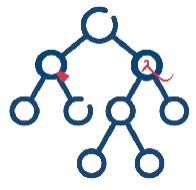
\includegraphics[height=1.0cm]{msca_logo.png}}%
    \end{center}

    \vspace{0.6cm}

    % Main title with Q logos on sides (with clickable links)
    \begin{center}
        \begin{minipage}{0.1\textwidth}
            \centering
            \href{https://quantlet.com}{
\includegraphics[height=1.1cm]{ql_logo.png}}
        \end{minipage}%
        \begin{minipage}{0.78\textwidth}
            \centering
            {\LARGE\bfseries\usebeamercolor[fg]{title}\inserttitle}

            \vspace{0.3cm}

            {\usebeamerfont{subtitle}\usebeamercolor[fg]{title}\insertsubtitle}
        \end{minipage}%
        \begin{minipage}{0.1\textwidth}
            \centering
            \href{https://quantinar.com}{
\includegraphics[height=1.1cm]{qr_logo.png}}
        \end{minipage}
    \end{center}

    \vspace{0.6cm}

    % Authors (left aligned)
    \hspace{0.5cm}{\usebeamerfont{author}\insertauthor}

    \vspace{0.3cm}

    % Institute/Affiliations (left aligned)
    \hspace{0.5cm}\begin{minipage}[t]{0.9\textwidth}
        \raggedright\small\insertinstitute
    \end{minipage}
}

%=============================================================================
% THEOREM ENVIRONMENTS
%=============================================================================
\theoremstyle{definition}
\setbeamertemplate{theorems}[numbered]
\ifdefined\atslang
\newtheorem{defn}{Definiție}
\newtheorem{thm}{Teoremă}
\newtheorem{prop}{Propoziție}
\newtheorem{rmk}{Observație}
\else
\newtheorem{defn}{Definition}
\newtheorem{thm}{Theorem}
\newtheorem{prop}{Proposition}
\newtheorem{rmk}{Remark}
\fi

%=============================================================================
% CENTRED MINIPAGE (no extra vertical space)
%=============================================================================
\newenvironment{cminipage}[1]{%
    \par\noindent\hfill\begin{minipage}{#1}\ignorespaces
}{%
    \end{minipage}\hfill\null\par
}

%=============================================================================
% CUSTOM COMMANDS
%=============================================================================
\newcommand{\E}{\mathbb{E}}
\newcommand{\Var}{\text{Var}}
\newcommand{\Cov}{\text{Cov}}
\newcommand{\Corr}{\text{Corr}}
\newcommand{\R}{\mathbb{R}}
\newcommand{\N}{\mathbb{N}}
\newcommand{\Z}{\mathbb{Z}}
\newcommand{\B}{\mathbf{B}}
\newcommand{\imark}{\textcolor{MainBlue}{\textbullet}}
\newcommand{\RMSE}{\text{RMSE}}
\newcommand{\MAE}{\text{MAE}}
\newcommand{\MAPE}{\text{MAPE}}

% Boldface vector/matrix commands (VAR, VECM, state space)
\newcommand{\bY}{\mathbf{Y}}
\newcommand{\bX}{\mathbf{X}}
\newcommand{\bA}{\mathbf{A}}
\newcommand{\bB}{\mathbf{B}}
\newcommand{\bepsilon}{\boldsymbol{\varepsilon}}
\newcommand{\bSigma}{\boldsymbol{\Sigma}}
\newcommand{\bPhi}{\boldsymbol{\Phi}}
\newcommand{\bGamma}{\boldsymbol{\Gamma}}
\newcommand{\bPi}{\boldsymbol{\Pi}}
\newcommand{\bc}{\mathbf{c}}
\newcommand{\balpha}{\boldsymbol{\alpha}}
\newcommand{\bbeta}{\boldsymbol{\beta}}
\newcommand{\bvarepsilon}{\boldsymbol{\varepsilon}}

% Seminar marks
\newcommand{\correct}{\textcolor{Forest}{\checkmark}}
\newcommand{\incorrect}{\textcolor{Crimson}{\texttimes}}
 se definește
%   \newcommand{\coursename}{Advanced Time Series Analysis and Forecasting}          (EN)
%   \newcommand{\coursename}{Analiza avansată a seriilor de timp și previziune}       (RO)  și  \def\atslang{ro}
% Fișierele .tex se află în EN/Courses, EN/Seminars, RO/Cursuri, RO/Seminarii (două niveluri sub rădăcină).
% Deck-urile sînt generate de latex/build_chapterN.py / build_seminarN.py (vezi latex/ats_build.py).

\documentclass[9pt, aspectratio=169, t]{beamer}
\providecommand{\coursename}{Advanced Time Series Analysis and Forecasting}

% Ensure content fits on slides
\setbeamersize{text margin left=8mm, text margin right=8mm}
% Smaller institute font (title page)
\setbeamerfont{institute}{size=\footnotesize}

%=============================================================================
% THEME AND STYLE CONFIGURATION
%=============================================================================
\usetheme{default}
% Using default theme for clean header/footer control

% Color Palette (matching Redispatch PDF)
\definecolor{MainBlue}{RGB}{26, 58, 110}
\definecolor{AccentBlue}{RGB}{26, 58, 110}
\definecolor{IDAred}{RGB}{205, 0, 0}
\definecolor{DarkGray}{RGB}{51, 51, 51}
\definecolor{MediumGray}{RGB}{128, 128, 128}
\definecolor{LightGray}{RGB}{248, 248, 248}
\definecolor{VeryLightGray}{RGB}{235, 235, 235}
\definecolor{KeynoteGray}{RGB}{218, 218, 218}
\definecolor{SectionGray}{RGB}{120, 120, 120}
\definecolor{FooterGray}{RGB}{100, 100, 100}
\definecolor{Crimson}{RGB}{220, 53, 69}
\definecolor{Forest}{RGB}{46, 125, 50}
\definecolor{Amber}{RGB}{181, 133, 63}
\definecolor{Orange}{RGB}{230, 126, 34}
\definecolor{Purple}{RGB}{142, 68, 173}

% Gradient background (exact Keynote 315° gradient: white to RGB 218,218,218)
\setbeamertemplate{background}{%
    \begin{tikzpicture}[remember picture, overlay]
        \shade[shading=axis, shading angle=315,
        top color=white, bottom color=KeynoteGray]
        (current page.south west) rectangle (current page.north east);
    \end{tikzpicture}%
}
% Fallback solid color for compatibility
\setbeamercolor{background canvas}{bg=}

\setbeamercolor{palette primary}{bg=MainBlue, fg=white}
\setbeamercolor{palette secondary}{bg=MainBlue!85, fg=white}
\setbeamercolor{palette tertiary}{bg=MainBlue!70, fg=white}
\setbeamercolor{structure}{fg=MainBlue}
\setbeamercolor{title}{fg=IDAred}
\setbeamercolor{frametitle}{fg=IDAred, bg=}
\setbeamercolor{block title}{bg=MainBlue, fg=white}
\setbeamercolor{block body}{bg=VeryLightGray, fg=DarkGray}
\setbeamercolor{block title alerted}{bg=Crimson, fg=white}
\setbeamercolor{block body alerted}{bg=Crimson!8, fg=DarkGray}
\setbeamercolor{block title example}{bg=Forest, fg=white}
\setbeamercolor{block body example}{bg=Forest!8, fg=DarkGray}
\setbeamercolor{item}{fg=MainBlue}

% Footer colors (override Madrid theme blue)
\setbeamercolor{author in head/foot}{fg=FooterGray, bg=}
\setbeamercolor{title in head/foot}{fg=FooterGray, bg=}
\setbeamercolor{date in head/foot}{fg=FooterGray, bg=}
\setbeamercolor{section in head/foot}{fg=FooterGray, bg=}
\setbeamercolor{subsection in head/foot}{fg=FooterGray, bg=}

% Bullet styles (apply everywhere including blocks)
\setbeamertemplate{itemize item}{\color{MainBlue}$\boxdot$}
\setbeamertemplate{itemize subitem}{\color{MainBlue}$\blacktriangleright$}
\setbeamertemplate{itemize subsubitem}{\color{MainBlue}\tiny$\bullet$}
\setbeamertemplate{itemize/enumerate body begin}{\normalsize}
\setbeamertemplate{itemize/enumerate subbody begin}{\normalsize}

% Item spacing - compact style
\setlength{\leftmargini}{10pt}       % Level 1: minimal indent
\setlength{\leftmarginii}{10pt}      % Level 2: minimal additional indent
% Compact list spacing (zero extra space before/after lists in blocks)
\makeatletter
\def\@listi{\leftmargin\leftmargini \topsep 0pt \parsep 0pt \itemsep 0pt}
\def\@listii{\leftmargin\leftmarginii \topsep 0pt \parsep 0pt \itemsep 0pt}
\makeatother

\setbeamertemplate{navigation symbols}{}

%=============================================================================
% CUSTOM HEADLINE
%=============================================================================
\setbeamertemplate{headline}{%
    \vskip10pt%
    \hbox to \paperwidth{%
        \hskip0.5cm%
        {\small\color{FooterGray}\renewcommand{\hyperlink}[2]{##2}\insertsectionhead}%
        \hfill%
        \textcolor{FooterGray}{\small\insertframenumber}%
        \hskip0.5cm%
    }%
    \vskip4pt%
    {\color{FooterGray}\hrule height 0.4pt}%
}

%=============================================================================
% CUSTOM FOOTER
%=============================================================================
\usepackage{fontawesome5}

\setbeamertemplate{footline}{%
    {\color{FooterGray}\hrule height 0.4pt}%
    \vskip4pt%
    \hbox to \paperwidth{%
        \hskip0.5cm%
        \textcolor{FooterGray}{\small\coursename}%
        \hfill%
        \raisebox{-0.1em}{%
            \begin{tikzpicture}[x=0.08em, y=0.08em, line width=0.4pt]
                \draw[FooterGray] (0,3) -- (1,4) -- (2,3.5) -- (3,5) -- (4,4) -- (5,6) -- (6,5.5) -- (7,4) -- (8,5) -- (9,7) -- (10,6) -- (11,5) -- (12,6.5) -- (13,8) -- (14,7) -- (15,6) -- (16,7.5) -- (17,9) -- (18,8) -- (19,7) -- (20,8.5) -- (21,10) -- (22,9) -- (23,8) -- (24,9.5);
            \end{tikzpicture}%
        }%
        \hskip0.5cm%
    }%
    \vskip6pt%
}

%=============================================================================
% PACKAGES
%=============================================================================
\usepackage[utf8]{inputenc}
\DeclareUnicodeCharacter{03B1}{\ensuremath{\alpha}}
\usepackage[T1]{fontenc}
\usepackage{amsmath, amssymb, amsthm}
\usepackage{mathtools}
\usepackage{bm}
\usepackage{tikz}
\usetikzlibrary{arrows.meta, positioning, shapes, calc, decorations.pathreplacing, shadings}
\usepackage{booktabs}
\usepackage{multirow}
\usepackage{array}
\usepackage{graphicx}
\usepackage{animate}
\usepackage{hyperref}
\usepackage{colortbl}
\usepackage{listings}
\lstset{language=Python, basicstyle=\ttfamily\scriptsize, keywordstyle=\color{MainBlue}\bfseries,
  commentstyle=\color{Forest}, stringstyle=\color{Crimson}, breaklines=true,
  frame=none, backgroundcolor=\color{VeryLightGray}, xleftmargin=2mm}
\hypersetup{colorlinks=true, linkcolor=MainBlue, urlcolor=MainBlue}
\graphicspath{{../../logos/}{../../charts/}{../../photos/}}
\usepackage{xcolor}
\hfuzz=2pt  % Suppress tiny overfull warnings (<2pt)
\vfuzz=2pt  % Suppress tiny vertical overfull warnings (<2pt)

%=============================================================================
% QUANTLET COMMANDS
%   \quantlet{<displayed name>}{<url>}       (generic)
%   \atsquantlet{Ch_05}{ATS_ch5_garch}       -> https://github.com/danpele/Advanced-Time-Series/tree/main/Quantlets/Ch_05/ATS_ch5_garch
%   \qlurl{<folder>} is defined per chapter by the generator (Quantlets/Ch_NN/<folder>)
%=============================================================================
\newcommand{\atsrepo}{https://github.com/danpele/Advanced-Time-Series}
\newcommand{\atsqlbase}{https://github.com/danpele/Advanced-Time-Series/tree/main/Quantlets}
\newcommand{\quantlet}[2]{%
    \hfill\href{#2}{%
        \raisebox{-0.15em}{
\includegraphics[height=0.7em]{ql_logo.png}}%
        \textcolor{MainBlue}{\tiny\ #1}%
    }%
}
\newcommand{\atsquantlet}[2]{\quantlet{\detokenize{#2}}{\atsqlbase/#1/#2}}

%=============================================================================
% NOTEBOOKS (Google Colab)
%   \colaburl{notebooks/EN/chapter5_seminar_notebook.ipynb} -> the Colab link of a file in the ATS repo
%   \nb: the chapter notebook (each seminar deck redefines it with \renewcommand)
%=============================================================================
\newcommand{\colaburl}[1]{https://colab.research.google.com/github/danpele/Advanced-Time-Series/blob/main/#1}
\newcommand{\nb}{https://colab.research.google.com/github/danpele/Advanced-Time-Series/tree/main/notebooks/EN}
\newcommand{\nbname}{notebooks/EN}

%=============================================================================
% SLIDE HELPERS (used by the generators; the same as in MFM)
%=============================================================================
% local font size for list bodies (the preamble forces \normalsize)
\newcommand{\itemsize}[1]{\setbeamertemplate{itemize/enumerate body begin}{#1}\setbeamertemplate{itemize/enumerate subbody begin}{#1}}
\newcommand{\intitle}[1]{{\hypersetup{urlcolor=white}#1}}   % white links inside coloured title bars
\newcommand{\imgcap}[1]{{\scriptsize #1}\\[0.5mm]}          % caption under a photo
\newcommand{\imgcredit}[2]{{\tiny\color{FooterGray}\href{#1}{#2}}}   % image credit: source URL, author/licence
\newcommand{\aiprompt}[1]{{\ttfamily\color{MainBlue}#1}}     % a prompt to an AI assistant

%=============================================================================
% SEMINARS: student version by default; the instructor wrapper *_solutions.tex sets \solutionstrue
%=============================================================================
\makeatletter\@ifundefined{ifsolutions}{\expandafter\newif\csname ifsolutions\endcsname}{}\makeatother
\newcommand{\solonly}[1]{\ifsolutions #1\fi}
\newcommand{\propsub}{\ifsolutions\else\framesubtitle{\ifdefined\atslang Rezolvarea se discută la seminar\else Solution discussed in class\fi}\fi}

%=============================================================================
% APPENDIX AND CHAPTER LINKS (latex/appendix_links.py writes the calls; it also re-declares these
% macros before \begin{document}, so the decks compile with or without this preamble block)
%=============================================================================
\providecommand{\atsapplink}[3]{\hypertarget{#2}{}\hyperlink{#1}{\beamergotobutton{#3}}}
\providecommand{\atsappback}[2]{\begin{tikzpicture}[remember picture,overlay]\node[anchor=south east] at ([xshift=-3mm,yshift=7mm]current page.south east){\hyperlink{#1}{\beamerreturnbutton{#2}}};\end{tikzpicture}}
\providecommand{\atschlink}[2]{\href{#1}{#2}}
\providecommand{\atschlinkt}[2]{\href{#1}{\usebeamercolor[fg]{frametitle}#2}}

%=============================================================================
% QUANTINAR COMMAND: link către un curs Quantinar (subiecte avansate)
%=============================================================================
\newcommand{\quantinar}[2]{%
    \href{#2}{%
        \raisebox{-0.15em}{
\includegraphics[height=0.8em]{qr_logo.png}}%
        \textcolor{MainBlue}{\scriptsize\ #1}%
    }%
}

%=============================================================================
% CUSTOM TITLE PAGE
%=============================================================================
\defbeamertemplate*{title page}{hybrid}[1][]
{
    \vspace{0.2cm}
    % Logos row - top header (with clickable links)
    \begin{center}
        \href{https://www.ase.ro}{
\includegraphics[height=1.0cm]{ase_logo.png}}\hspace{0.3cm}%
        \href{https://theida.net}{
\includegraphics[height=1.0cm]{ida_logo.png}}\hspace{0.3cm}%
        \href{https://blockchain-research-center.com}{
\includegraphics[height=1.0cm]{brc_logo.png}}\hspace{0.3cm}%
        \href{https://www.ai4efin.ase.ro}{
\includegraphics[height=1.0cm]{ai4efin_logo.png}}\hspace{0.3cm}%
        \href{https://ipe.ro/new}{
\includegraphics[height=1.0cm]{acad_logo.png}}\hspace{0.3cm}%
        \href{https://www.digital-finance-msca.com}{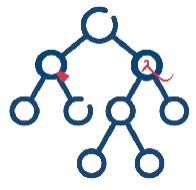
\includegraphics[height=1.0cm]{msca_logo.png}}%
    \end{center}

    \vspace{0.6cm}

    % Main title with Q logos on sides (with clickable links)
    \begin{center}
        \begin{minipage}{0.1\textwidth}
            \centering
            \href{https://quantlet.com}{
\includegraphics[height=1.1cm]{ql_logo.png}}
        \end{minipage}%
        \begin{minipage}{0.78\textwidth}
            \centering
            {\LARGE\bfseries\usebeamercolor[fg]{title}\inserttitle}

            \vspace{0.3cm}

            {\usebeamerfont{subtitle}\usebeamercolor[fg]{title}\insertsubtitle}
        \end{minipage}%
        \begin{minipage}{0.1\textwidth}
            \centering
            \href{https://quantinar.com}{
\includegraphics[height=1.1cm]{qr_logo.png}}
        \end{minipage}
    \end{center}

    \vspace{0.6cm}

    % Authors (left aligned)
    \hspace{0.5cm}{\usebeamerfont{author}\insertauthor}

    \vspace{0.3cm}

    % Institute/Affiliations (left aligned)
    \hspace{0.5cm}\begin{minipage}[t]{0.9\textwidth}
        \raggedright\small\insertinstitute
    \end{minipage}
}

%=============================================================================
% THEOREM ENVIRONMENTS
%=============================================================================
\theoremstyle{definition}
\setbeamertemplate{theorems}[numbered]
\ifdefined\atslang
\newtheorem{defn}{Definiție}
\newtheorem{thm}{Teoremă}
\newtheorem{prop}{Propoziție}
\newtheorem{rmk}{Observație}
\else
\newtheorem{defn}{Definition}
\newtheorem{thm}{Theorem}
\newtheorem{prop}{Proposition}
\newtheorem{rmk}{Remark}
\fi

%=============================================================================
% CENTRED MINIPAGE (no extra vertical space)
%=============================================================================
\newenvironment{cminipage}[1]{%
    \par\noindent\hfill\begin{minipage}{#1}\ignorespaces
}{%
    \end{minipage}\hfill\null\par
}

%=============================================================================
% CUSTOM COMMANDS
%=============================================================================
\newcommand{\E}{\mathbb{E}}
\newcommand{\Var}{\text{Var}}
\newcommand{\Cov}{\text{Cov}}
\newcommand{\Corr}{\text{Corr}}
\newcommand{\R}{\mathbb{R}}
\newcommand{\N}{\mathbb{N}}
\newcommand{\Z}{\mathbb{Z}}
\newcommand{\B}{\mathbf{B}}
\newcommand{\imark}{\textcolor{MainBlue}{\textbullet}}
\newcommand{\RMSE}{\text{RMSE}}
\newcommand{\MAE}{\text{MAE}}
\newcommand{\MAPE}{\text{MAPE}}

% Boldface vector/matrix commands (VAR, VECM, state space)
\newcommand{\bY}{\mathbf{Y}}
\newcommand{\bX}{\mathbf{X}}
\newcommand{\bA}{\mathbf{A}}
\newcommand{\bB}{\mathbf{B}}
\newcommand{\bepsilon}{\boldsymbol{\varepsilon}}
\newcommand{\bSigma}{\boldsymbol{\Sigma}}
\newcommand{\bPhi}{\boldsymbol{\Phi}}
\newcommand{\bGamma}{\boldsymbol{\Gamma}}
\newcommand{\bPi}{\boldsymbol{\Pi}}
\newcommand{\bc}{\mathbf{c}}
\newcommand{\balpha}{\boldsymbol{\alpha}}
\newcommand{\bbeta}{\boldsymbol{\beta}}
\newcommand{\bvarepsilon}{\boldsymbol{\varepsilon}}

% Seminar marks
\newcommand{\correct}{\textcolor{Forest}{\checkmark}}
\newcommand{\incorrect}{\textcolor{Crimson}{\texttimes}}


\newcommand{\qlurl}[1]{https://github.com/danpele/Advanced-Time-Series/tree/main/Quantlets/Ch_15/#1}

% Clickable citations (DOIs verified via Crossref)
\newcommand{\refNW}{\href{https://doi.org/10.2307/1913610}{Newey și West (1987)}}
\newcommand{\refEH}{\href{https://doi.org/10.1111/j.1540-6261.1991.tb02674.x}{Estrella și Hardouvelis (1991)}}
\newcommand{\refWhite}{\href{https://doi.org/10.1111/1468-0262.00152}{White (2000)}}
\newcommand{\refMR}{\href{https://doi.org/10.1016/0022-1996(83)90017-X}{Meese și Rogoff (1983)}}
\newcommand{\refGKMT}{\href{https://doi.org/10.1016/j.ijforecast.2012.06.004}{Genre et al.\ (2013)}}
\newcommand{\refAO}{\href{https://doi.org/10.21034/qr.2511}{Atkeson și Ohanian (2001)}}
\newcommand{\refDM}{\href{https://doi.org/10.1080/07350015.1995.10524599}{Diebold și Mariano (1995)}}
\newcommand{\refHLN}{\href{https://doi.org/10.1016/S0169-2070(96)00719-4}{Harvey, Leybourne și Newbold (1997)}}
\newcommand{\refCW}{\href{https://doi.org/10.1016/j.jeconom.2006.05.023}{Clark și West (2007)}}
\newcommand{\refMPQ}{\href{https://doi.org/10.1257/aer.90.5.1464}{McConnell și Perez-Quiros (2000)}}
\newcommand{\refBP}{\href{https://doi.org/10.1002/jae.659}{Bai și Perron (2003)}}
\newcommand{\refHanB}{\href{https://doi.org/10.2202/1558-3708.1024}{Hansen (1997)}}
\newcommand{\refTPS}{\href{https://doi.org/10.1111/1468-2354.00144}{Taylor, Peel și Sarno (2001)}}
\newcommand{\refCEE}{\href{https://doi.org/10.1016/S1574-0048(99)01005-8}{Christiano, Eichenbaum și Evans (1999)}}
\newcommand{\refGK}{\href{https://doi.org/10.1257/mac.20130329}{Gertler și Karadi (2015)}}
\newcommand{\refKil}{\href{https://doi.org/10.1257/aer.99.3.1053}{Kilian (2009)}}
\newcommand{\refKPSW}{\href{https://www.jstor.org/stable/2006644}{King, Plosser, Stock și Watson (1991)}}
\newcommand{\refPSS}{\href{https://doi.org/10.1080/01621459.1999.10474156}{Pesaran, Shin și Smith (1999)}}
\newcommand{\refBGR}{\href{https://doi.org/10.1002/jae.1137}{Bańbura, Giannone și Reichlin (2010)}}
\newcommand{\refSW}{\href{https://doi.org/10.1198/073500102317351921}{Stock și Watson (2002)}}
\newcommand{\refMNZ}{\href{https://doi.org/10.1162/003465303765299765}{Morley, Nelson și Zivot (2003)}}
\newcommand{\refHam}{\href{https://doi.org/10.2307/1912559}{Hamilton (1989)}}
\newcommand{\refEGS}{\href{https://doi.org/10.1162/REST_a_00300}{Engle, Ghysels și Sohn (2013)}}
\newcommand{\refBPQ}{\href{https://doi.org/10.1016/j.jeconom.2015.10.007}{Bollerslev, Patton și Quaedvlieg (2016)}}
\newcommand{\refELW}{\href{https://doi.org/10.1080/07350015.2017.1345683}{Engle, Ledoit și Wolf (2019)}}
\newcommand{\refPZC}{\href{https://doi.org/10.1016/j.jeconom.2018.10.008}{Patton, Ziegel și Chen (2019)}}
\newcommand{\refEM}{\href{https://doi.org/10.1198/073500104000000370}{Engle și Manganelli (2004)}}
\newcommand{\refGJR}{\href{https://doi.org/10.1080/14697688.2017.1393551}{Gatheral, Jaisson și Rosenbaum (2018)}}
\newcommand{\refQu}{\href{https://doi.org/10.1198/jbes.2010.09153}{Qu (2011)}}
\newcommand{\refCN}{\href{https://doi.org/10.1016/0165-1889(93)00781-X}{Cogley și Nason (1995)}}
\newcommand{\refHamB}{\href{https://doi.org/10.1162/rest_a_00706}{Hamilton (2018)}}
\newcommand{\refBHK}{\href{https://doi.org/10.1016/j.csda.2017.11.003}{Bergmeir, Hyndman și Koo (2018)}}
\newcommand{\refZeng}{\href{https://doi.org/10.1609/aaai.v37i9.26317}{Zeng et al.\ (2023)}}
\newcommand{\refNie}{\href{https://arxiv.org/abs/2211.14730}{Nie et al.\ (2023)}}
\newcommand{\refGC}{\href{https://arxiv.org/abs/2106.00170}{Gibbs și Candès (2021)}}
\newcommand{\refRPC}{\href{https://arxiv.org/abs/1905.03222}{Romano, Patterson și Candès (2019)}}
\newcommand{\refADH}{\href{https://doi.org/10.1111/ajps.12116}{Abadie, Diamond și Hainmueller (2015)}}
\newcommand{\refBMSS}{\href{https://doi.org/10.1093/ej/uez020}{Born et al.\ (2019)}}
\newcommand{\refPWY}{\href{https://doi.org/10.1111/j.1468-2354.2010.00625.x}{Phillips, Wu și Yu (2011)}}
\newcommand{\refPSY}{\href{https://doi.org/10.1111/iere.12132}{Phillips, Shi și Yu (2015)}}
\newcommand{\refPY}{\href{https://doi.org/10.3982/QE82}{Phillips și Yu (2011)}}
\newcommand{\refHLST}{\href{https://doi.org/10.1016/j.jempfin.2015.09.002}{Harvey et al.\ (2016)}}
\newcommand{\refHansen}{\href{https://doi.org/10.1198/073500105000000063}{Hansen (2005)}}
\newcommand{\refHLNa}{\href{https://doi.org/10.3982/ECTA5771}{Hansen, Lunde și Nason (2011)}}
\newcommand{\refRW}{\href{https://doi.org/10.1111/j.1468-0262.2005.00615.x}{Romano și Wolf (2005)}}
\newcommand{\refKV}{\href{https://doi.org/10.1017/S0266466605050565}{Kiefer și Vogelsang (2005)}}
\newcommand{\refLLSW}{\href{https://doi.org/10.1080/07350015.2018.1506926}{Lazarus et al.\ (2018)}}
\newcommand{\refIK}{\href{https://doi.org/10.1081/ETC-200040785}{Inoue și Kilian (2005)}}
\newcommand{\refDiebold}{\href{https://doi.org/10.1080/07350015.2014.983236}{Diebold (2015)}}
\newcommand{\refStam}{\href{https://doi.org/10.1016/S0304-405X(99)00041-0}{Stambaugh (1999)}}
\newcommand{\refWG}{\href{https://doi.org/10.1093/rfs/hhm014}{Welch și Goyal (2008)}}
\newcommand{\refSNS}{\href{https://doi.org/10.1177/0956797611417632}{Simmons, Nelson și Simonsohn (2011)}}
\newcommand{\refGL}{\href{https://doi.org/10.1511/2014.111.460}{Gelman și Loken (2014)}}
\newcommand{\refHLZ}{\href{https://doi.org/10.1093/rfs/hhv059}{Harvey, Liu și Zhu (2016)}}
\newcommand{\refIoa}{\href{https://doi.org/10.1371/journal.pmed.0020124}{Ioannidis (2005)}}
\newcommand{\refBLSZ}{\href{https://doi.org/10.1257/app.20150044}{Brodeur et al.\ (2016)}}
\newcommand{\refNos}{\href{https://doi.org/10.1073/pnas.1708274114}{Nosek et al.\ (2018)}}
\newcommand{\refKau}{\href{https://doi.org/10.1145/2382577.2382579}{Kaufman et al.\ (2012)}}
\newcommand{\refCle}{\href{https://doi.org/10.1111/joes.12139}{Clemens (2017)}}
\newcommand{\refCM}{\href{https://doi.org/10.1257/jel.20171350}{Christensen și Miguel (2018)}}
\newcommand{\refVil}{\href{https://doi.org/10.1162/99608f92.4f6b9e67}{Vilhuber (2020)}}
\newcommand{\refCL}{\href{https://doi.org/10.1561/104.00000053}{Chang și Li (2022)}}
\newcommand{\refHAP}{\href{https://doi.org/10.1093/cje/bet075}{Herndon, Ash și Pollin (2014)}}
\newcommand{\refHXZ}{\href{https://doi.org/10.1093/rfs/hhy131}{Hou, Xue și Zhang (2020)}}
\newcommand{\refMen}{\href{https://doi.org/10.1111/jofi.13337}{Menkveld et al.\ (2024)}}
\newcommand{\refSil}{\href{https://doi.org/10.1177/2515245917747646}{Silberzahn et al.\ (2018)}}
\newcommand{\refSSN}{\href{https://doi.org/10.1038/s41562-020-0912-z}{Simonsohn, Simmons și Nelson (2020)}}
\newcommand{\refSte}{\href{https://doi.org/10.1177/1745691616658637}{Steegen et al.\ (2016)}}
\newcommand{\refPeng}{\href{https://doi.org/10.1126/science.1213847}{Peng (2011)}}
\newcommand{\refPet}{\href{https://doi.org/10.1016/j.ijforecast.2021.11.001}{Petropoulos et al.\ (2022)}}
\newcommand{\refMC}{\href{https://doi.org/10.1038/s41586-024-07146-0}{Messeri și Crockett (2024)}}
\newcommand{\refWW}{\href{https://doi.org/10.1038/s41598-023-41032-5}{Walters și Wilder (2023)}}
\newcommand{\refKor}{\href{https://doi.org/10.1257/jel.20231736}{Korinek (2023)}}
\newcommand{\refWang}{\href{https://doi.org/10.1038/s41586-023-06221-2}{Wang et al.\ (2023)}}
\newcommand{\refLu}{\href{https://arxiv.org/abs/2408.06292}{Lu et al.\ (2024)}}

\title[Analiza avansată a seriilor de timp și previziune]{Analiza avansată a seriilor de timp și previziune}
\subtitle{Capitolul 15: Recapitulare și susținerea proiectelor}
\author[D.T. Pele]{Daniel Traian PELE}
\institute{Academia de Studii Economice din București\\
IDA Institute Digital Assets\\
Blockchain Research Center\\
AI4EFin Artificial Intelligence for Energy Finance\\
Academia Română, Institutul de Prognoză Economică\\
MSCA Digital Finance}
\date{}

%=============================================================================
\providecommand{\atsapplink}[3]{\hypertarget{#2}{}\hyperlink{#1}{\beamergotobutton{#3}}}  % APPLINKS-MACROS
\providecommand{\atsappback}[2]{\begin{tikzpicture}[remember picture,overlay]\node[anchor=south east] at ([xshift=-3mm,yshift=7mm]current page.south east){\hyperlink{#1}{\beamerreturnbutton{#2}}};\end{tikzpicture}}  % APPLINKS-MACROS
\providecommand{\atschlink}[2]{\href{#1}{#2}}  % APPLINKS-MACROS
\providecommand{\atschlinkt}[2]{\href{#1}{\usebeamercolor[fg]{frametitle}#2}}  % APPLINKS-MACROS
\begin{document}
%=============================================================================

{
\setbeamertemplate{headline}{}
\setbeamertemplate{footline}{}
\begin{frame}[noframenumbering]
    \titlepage
\end{frame}
}
% BEGIN-ACRONYMS (generat de latex/acronyms.py; nu editati manual)
\begin{frame}{Acronime folosite în acest material (1/4)}
\setbeamertemplate{itemize/enumerate body begin}{\tiny}
\begin{columns}[T]
\begin{column}{0.49\textwidth}
\begin{itemize}\setlength{\itemsep}{0pt}
    \item \textbf{ACI}: Adaptive Conformal Inference (inferență conformală adaptivă)
    \item \textbf{ADF}: Augmented Dickey–Fuller (test) — testul Dickey–Fuller augmentat
    \item \textbf{AI}: Artificial Intelligence (inteligență artificială)
    \item \textbf{ALFRED}: ArchivaL Federal Reserve Economic Data (arhiva vintage-urilor FRED (Fed St. Louis))
    \item \textbf{AR}: AutoRegressive (model); in event studies: Abnormal Return (model autoregresiv; în studiile de eveniment: randament anormal)
    \item \textbf{ARDL}: AutoRegressive Distributed Lag (model) — model autoregresiv cu decalaje distribuite
    \item \textbf{ARX}: AutoRegressive model with eXogenous variables (model autoregresiv cu variabile exogene)
    \item \textbf{BCE}: Banca Centrală Europeană
    \item \textbf{BET}: Bucharest Exchange Trading (index) — indicele de referință al Bursei de Valori București
    \item \textbf{BH}: Benjamini–Hochberg (procedure) — procedura Benjamini–Hochberg
    \item \textbf{BNR}: Banca Națională a României
    \item \textbf{BSADF}: Backward Supremum Augmented Dickey–Fuller (statistic) — statistica ADF supremum retrospectivă, pentru fiecare dată de sfîrșit
    \item \textbf{BVAR}: Bayesian Vector AutoRegression (model vector autoregresiv bayesian)
\end{itemize}
\end{column}
\begin{column}{0.49\textwidth}
\begin{itemize}\setlength{\itemsep}{0pt}
    \item \textbf{CCE}: Common Correlated Effects (estimator) — estimatorul efectelor comune corelate
    \item \textbf{CCM}: Convergent Cross Mapping (estimare încrucișată convergentă (Sugihara et al. 2012))
    \item \textbf{CQR}: Conformalized Quantile Regression (regresia cuantilică conformalizată)
    \item \textbf{CRPS}: Continuous Ranked Probability Score (scorul probabilistic continuu)
    \item \textbf{CSW}: Chu, Stinchcombe and White (monitoring boundary) — Chu, Stinchcombe și White (frontiera de monitorizare)
    \item \textbf{DCC}: Dynamic Conditional Correlation (corelație condiționată dinamică)
    \item \textbf{DCC-NL}: DCC with Nonlinear shrinkage of the target (Engle–Ledoit–Wolf 2019) — DCC cu shrinkage neliniar al țintei (Engle–Ledoit–Wolf 2019)
    \item \textbf{DFM}: Dynamic Factor Model (model factorial dinamic)
    \item \textbf{DM}: Diebold–Mariano (test) — testul Diebold–Mariano de comparare a prognozelor
    \item \textbf{DQ}: Dynamic Quantile (test of Engle and Manganelli) — testul dinamic pe cuantile al lui Engle și Manganelli
    \item \textbf{ECE}: Europa Centrală și de Est
    \item \textbf{EM}: Expectation–Maximisation (algorithm) — algoritmul expectație–maximizare
    \item \textbf{EODHD}: EOD Historical Data (market-data provider) — furnizor de date de piață
\end{itemize}
\end{column}
\end{columns}
\end{frame}
\begin{frame}{Acronime folosite în acest material (2/4)}
\setbeamertemplate{itemize/enumerate body begin}{\tiny}
\begin{columns}[T]
\begin{column}{0.49\textwidth}
\begin{itemize}\setlength{\itemsep}{0pt}
    \item \textbf{ES}: Expected Shortfall (pierderea așteptată în coadă)
    \item \textbf{EWC}: Equal-Weighted Cosine (estimator) — estimatorul cu cosinusuri ponderate egal
    \item \textbf{FRED}: Federal Reserve Economic Data (baza de date economice a Rezervei Federale din St. Louis)
    \item \textbf{FZ0}: Zero-homogeneous Fissler–Ziegel loss (Patton, Ziegel and Chen) — pierderea Fissler–Ziegel omogenă de grad zero (Patton, Ziegel și Chen)
    \item \textbf{GARCH}: Generalised AutoRegressive Conditional Heteroskedasticity (heteroscedasticitate condiționată autoregresivă generalizată)
    \item \textbf{GAS-1F}: One-factor GAS model for VaR and ES (model GAS cu un factor pentru VaR și ES)
    \item \textbf{GMV}: Global Minimum-Variance (portfolio) — portofoliul de varianță minimă globală
    \item \textbf{GSADF}: Generalised Supremum Augmented Dickey–Fuller (test) — testul ADF supremum generalizat (toate începuturile și sfîrșiturile)
    \item \textbf{HAC}: Heteroskedasticity and Autocorrelation Consistent (standard errors) — erori standard robuste la heteroscedasticitate și autocorelație
    \item \textbf{HAR}: Heterogeneous AutoRegressive (model) — model autoregresiv heterogen
    \item \textbf{HARQ}: HAR with realised Quarticity (HAR cu cuarticitatea realizată)
    \item \textbf{HLN}: Harvey–Leybourne–Newbold (small-sample correction of the DM test) — corecția Harvey–Leybourne–Newbold a testului DM pentru eșantioane mici
    \item \textbf{HP}: Hodrick–Prescott (filter) — filtrul Hodrick–Prescott
\end{itemize}
\end{column}
\begin{column}{0.49\textwidth}
\begin{itemize}\setlength{\itemsep}{0pt}
    \item \textbf{IG}: inverse gamma (distribution) — distribuția inverse gamma
    \item \textbf{INS}: Institutul Național de Statistică
    \item \textbf{IPC}: Indicele prețurilor de consum
    \item \textbf{ITS}: Interrupted Time Series (serie de timp întreruptă)
    \item \textbf{LLM}: Large Language Model (model lingvistic de mari dimensiuni)
    \item \textbf{LM}: Lagrange Multiplier (multiplicatorul Lagrange)
    \item \textbf{LP}: Local Projection (proiecție locală)
    \item \textbf{LP-IV}: Local Projection with Instrumental Variables (proiecție locală cu variabile instrumentale)
    \item \textbf{LR}: Likelihood Ratio (test) — testul raportului de verosimilitate
    \item \textbf{MAE}: Mean Absolute Error (eroarea absolută medie)
    \item \textbf{MCO}: Metoda celor mai mici pătrate obișnuite
    \item \textbf{MCS}: Model Confidence Set (mulțimea de încredere a modelelor)
    \item \textbf{MGARCH}: Multivariate GARCH (GARCH multivariat)
\end{itemize}
\end{column}
\end{columns}
\end{frame}
\begin{frame}{Acronime folosite în acest material (3/4)}
\setbeamertemplate{itemize/enumerate body begin}{\tiny}
\begin{columns}[T]
\begin{column}{0.49\textwidth}
\begin{itemize}\setlength{\itemsep}{0pt}
    \item \textbf{MIDAS}: MIxed DAta Sampling (regression) — regresie cu date de frecvențe mixte
    \item \textbf{MNZ}: Morley–Nelson–Zivot (2003) — Morley–Nelson–Zivot (2003)
    \item \textbf{MSE}: Mean Squared Error (eroarea pătratică medie)
    \item \textbf{MSFE}: Mean Squared Forecast Error (eroarea medie pătratică de prognoză)
    \item \textbf{OECD}: Organisation for Economic Co-operation and Development (Organizația pentru Cooperare și Dezvoltare Economică)
    \item \textbf{OWA}: Overall Weighted Average (of sMAPE and MASE relative to Naive 2) — media ponderată generală a sMAPE și MASE relative la Naive 2
    \item \textbf{PCMCI}: PC algorithm + Momentary Conditional Independence (algoritmul PC urmat de testul de independență condiționată momentană (Runge et al. 2019))
    \item \textbf{PIB}: Produsul intern brut
    \item \textbf{PID}: Proportional--Integral--Derivative (controller) — controler proporțional--integral--derivat
    \item \textbf{PIT}: Probability Integral Transform (transformarea integrală de probabilitate)
    \item \textbf{PMG}: Pooled Mean Group (estimator) — estimatorul pooled mean group (termen lung comun, termen scurt eterogen)
    \item \textbf{QLIKE}: Quasi-LIKElihood loss (pierderea de tip cvasi-verosimilitate)
    \item \textbf{QML}: Quasi-Maximum Likelihood (verosimilitate cvasi-maximă)
\end{itemize}
\end{column}
\begin{column}{0.49\textwidth}
\begin{itemize}\setlength{\itemsep}{0pt}
    \item \textbf{QPS}: Quadratic Probability Score (scorul pătratic al probabilităților)
    \item \textbf{RMSE}: Root Mean Squared Error (rădăcina erorii pătratice medii)
    \item \textbf{RMSPE}: Root Mean Squared Prediction Error (rădăcina erorii pătratice medii de predicție)
    \item \textbf{SAV}: Symmetric Absolute Value (CAViaR specification) — specificația CAViaR cu valoare absolută simetrică
    \item \textbf{SC}: Synthetic Control (control sintetic)
    \item \textbf{SPA}: Superior Predictive Ability (test) — testul abilității predictive superioare
    \item \textbf{SPF}: Survey of Professional Forecasters (ancheta specialiștilor în prognoză (Survey of Professional Forecasters))
    \item \textbf{STAR}: Smooth Transition AutoRegression (autoregresie cu tranziție netedă)
    \item \textbf{SUA}: Statele Unite ale Americii
    \item \textbf{SVAR}: Structural Vector AutoRegression (model vector autoregresiv structural)
    \item \textbf{TAR}: Threshold AutoRegression (autoregresie cu prag)
    \item \textbf{TE}: Transfer Entropy (entropia de transfer)
    \item \textbf{TPS}: Taylor, Peel and Sarno (2001) — Taylor, Peel și Sarno (2001)
\end{itemize}
\end{column}
\end{columns}
\end{frame}
\begin{frame}{Acronime folosite în acest material (4/4)}
\setbeamertemplate{itemize/enumerate body begin}{\tiny}
\begin{columns}[T]
\begin{column}{0.49\textwidth}
\begin{itemize}\setlength{\itemsep}{0pt}
    \item \textbf{UC-SV}: Unobserved Components model with Stochastic Volatility (Stock–Watson 2007) — model cu componente neobservate și volatilitate stochastică (Stock–Watson 2007)
    \item \textbf{UC0}: UC model with uncorrelated trend and cycle shocks (Clark 1987) — model UC cu șocuri necorelate ale trendului și ciclului (Clark 1987)
    \item \textbf{UE}: Uniunea Europeană
    \item \textbf{UE-27}: cele 27 de state membre ale Uniunii Europene
    \item \textbf{VAR}: Vector AutoRegression (model vector autoregresiv)
    \item \textbf{VECM}: Vector Error Correction Model (model vectorial cu corecția erorii)
\end{itemize}
\end{column}
\begin{column}{0.49\textwidth}
\end{column}
\end{columns}
\end{frame}
% END-ACRONYMS

\begin{frame}{Întrebarea de azi și traseul}
\itemsize{\small}
\begin{columns}[T]
\begin{column}{0.58\textwidth}
\begin{itemize}
    \item \textbf{Întrebarea}: ce vă oferă întregul curs pentru un proiect de cercetare și cum se susține proiectul?
    \begin{itemize}
        \item un capitol care leagă \atschlink{https://danpele.github.io/Advanced-Time-Series/RO/Cursuri/capitol0_recapitulare_inferenta.pdf}{Capitolele 0}--\atschlink{https://danpele.github.io/Advanced-Time-Series/RO/Cursuri/capitol14_inferenta_cauzala_serii_timp.pdf}{14} și \atschlink{https://danpele.github.io/Advanced-Time-Series/RO/Cursuri/capitol16_radacini_explozive_bule_speculative.pdf}{Capitolul 16} (studiu individual) de proiectul de echipă
    \end{itemize}
    \item \textbf{Traseul}
    \begin{itemize}
        \item Partea I: harta cursului, cîte o recapitulare pentru fiecare capitol, trusa de metode
        \item Partea a II-a: fluxul de cercetare, replicarea unei lucrări de referință, lista de verificare a reproductibilității, erorile frecvente
        \item Partea a III-a: susținerea orală, AI în cercetare și alegerea proiectului
    \end{itemize}
    \item Cursul nu are examen scris: proiectul și susținerea lui reprezintă 70\% din notă
\end{itemize}
\end{column}
\begin{column}{0.38\textwidth}
\centering
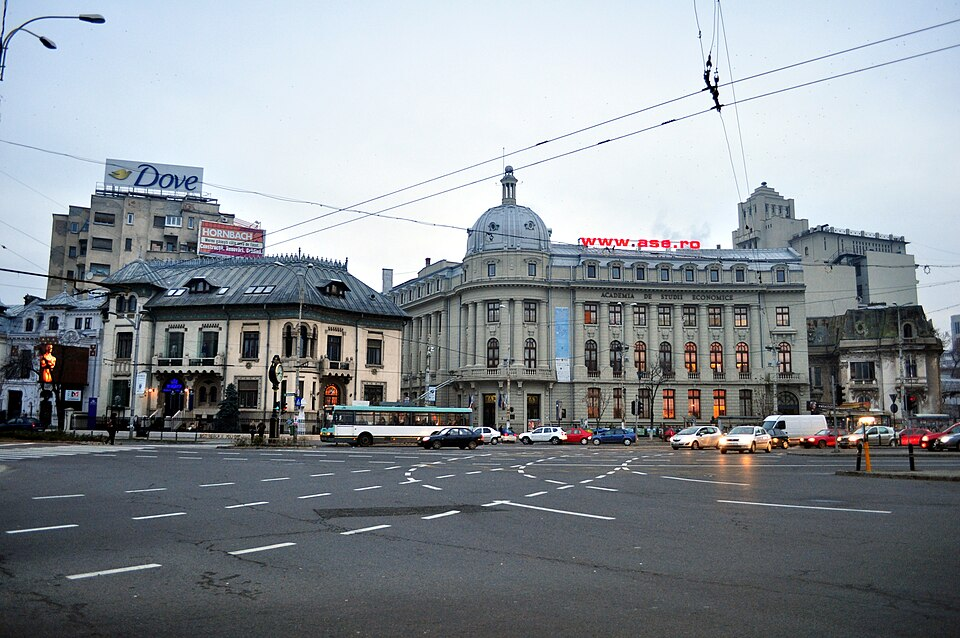
\includegraphics[height=0.40\textheight]{ch0_ase_2014.jpg}\\[1mm]
\imgcap{Academia de Studii Economice din București}
\imgcredit{https://commons.wikimedia.org/wiki/File:Bucharest_-_Academie_de_Studii_Economice_01.jpg}{Foto: Joe Mabel (2014); CC BY 3.0; Wikimedia Commons}
\end{column}
\end{columns}
\end{frame}

\begin{frame}{Rezultatele învățării}
\itemsize{\small}
\begin{itemize}
    \item Plasați fiecare capitol pe harta metodelor și formulați ideea-cheie, formula-cheie și rezultatul replicării
    \item Alegeți instrumentul potrivit pentru o întrebare de cercetare despre date dependente
    \item Planificați un proiect de la întrebare la raport, cu preînregistrare și calculul puterii evaluării
    \item Replicați o lucrare de referință, explicați o replicare nereușită și faceți reproductibil fiecare rezultat numeric
    \item Recunoașteți data snooping, leakage, look-ahead, p-hacking și afirmațiile exagerate în propria lucrare
    \item Pregătiți susținerea orală individuală și documentați folosirea instrumentelor AI
\end{itemize}
\end{frame}

\begin{frame}{Evaluarea pe scurt}
\itemsize{\small}
\begin{center}
\footnotesize
\begin{tabular}{>{\raggedright\arraybackslash}p{3.6cm}>{\raggedright\arraybackslash}p{1.4cm}>{\raggedright\arraybackslash}p{1.6cm}>{\raggedright\arraybackslash}p{6.6cm}}
\toprule
\textbf{Componenta} & \textbf{Pondere} & \textbf{Cine} & \textbf{Conținut} \\
\midrule
Propunerea și preînregistrarea & 5\% & echipa & întrebarea, lucrarea replicată, datele, designul evaluării fixat înaintea estimării \\
Replicarea și extensia & 15\% & echipa & repository, raport în forma unui articol, AI\_USE.md, AI\_ERRORS.md \\
Susținerea orală & 50\% & fiecare student & circa 15 minute: 5 minute de prezentare a contribuției proprii și 10 minute de întrebări despre cod, metodă și rezultate \\
Quiz-uri pe capitole & 20\% & fiecare student & online, se notează prima încercare \\
Prezență & 10\% & fiecare student & cursuri și seminarii \\
\bottomrule
\end{tabular}
\end{center}
\begin{itemize}
    \item Echipe de cel mult trei studenți; proiectul se poate redacta și susține în română sau în engleză
    \item Notele membrilor unei echipe pot fi diferite: jumătate din nota finală este individuală
\end{itemize}
\end{frame}


%=============================================================================
\section{Harta cursului}
%=============================================================================

\begin{frame}{Harta cursului}
\itemsize{\footnotesize}
\hyphenpenalty=10000\relax
\begin{center}
\begin{tikzpicture}[font=\tiny, box/.style={draw=MainBlue, rounded corners=2pt, fill=MainBlue!6, align=center, text width=2.75cm, minimum height=0.55cm, inner sep=2pt},
  base/.style={box, draw=Forest, fill=Forest!8, text width=3.6cm}, proj/.style={box, draw=IDAred, fill=IDAred!8, text width=3.2cm, font=\scriptsize},
  head/.style={font=\scriptsize\bfseries, text=MainBlue, align=center, text width=2.9cm}, ar/.style={-{Stealth[length=1.6mm]}, MainBlue!70, thick}]
\node[base] (c0) at (-2.1,2.75) {\textbf{0} Inferență pentru date dependente};
\node[base] (c1) at (2.1,2.75) {\textbf{1} Evaluarea și combinarea prognozelor};
\node[head] (h1) at (-4.95,1.85) {Structură și identificare};
\node[head] (h2) at (-1.65,1.85) {Stări latente};
\node[head] (h3) at (1.65,1.85) {Volatilitate și risc};
\node[head] (h4) at (4.95,1.85) {Frecvență și învățare};
\node[box] (c2) at (-4.95,1.2) {\textbf{2} Rupturi și modele neliniare};
\node[box] (c3) at (-4.95,0.5) {\textbf{3} SVAR și proiecții locale};
\node[box] (c4) at (-4.95,-0.2) {\textbf{4} Cointegrare, VECM, ARDL, panel};
\node[box] (c5) at (-4.95,-0.9) {\textbf{5} BVAR, factori, nowcasting};
\node[box] (c6) at (-1.65,1.2) {\textbf{6} Spațiul stărilor și filtrare bayesiană};
\node[box] (c7) at (-1.65,0.5) {\textbf{7} Schimbare de regim};
\node[box] (c8) at (1.65,1.2) {\textbf{8} Măsuri realizate, HAR, MGARCH};
\node[box] (c9) at (1.65,0.5) {\textbf{9} VaR, ES și backtesting};
\node[box] (c10) at (1.65,-0.2) {\textbf{10} Memorie lungă și rough volatility};
\node[box] (c11) at (4.95,1.2) {\textbf{11} Analiză spectrală și wavelet};
\node[box] (c12) at (4.95,0.5) {\textbf{12} Machine și deep learning};
\node[box] (c13) at (4.95,-0.2) {\textbf{13} Foundation models, conformal};
\node[box] (c14) at (-3.3,-1.95) {\textbf{14} Inferență cauzală pentru serii de timp};
\node[box] (c16) at (0,-1.95) {\textbf{16} Rădăcini explozive și bule (studiu individual)};
\node[proj] (c15) at (3.6,-1.95) {\textbf{15} Proiect: replicare, extensie, susținere};
\draw[ar] (c0.south) -- (h1.north); \draw[ar] (c0.south) -- (h2.north); \draw[ar] (c1.south) -- (h3.north); \draw[ar] (c1.south) -- (h4.north);
\draw[ar] (c0) -- (c1);
\draw[ar] (c16) -- (c15); \draw[ar] (c14.north east) to[out=20, in=160] (c15.north west);
\draw[ar, dashed] (c5.south) to[out=-90, in=150] (c14.north west);
\draw[ar, dashed] (c13.south) to[out=-90, in=60] (c15.north);
\end{tikzpicture}
\end{center}
\begin{itemize}
    \item \atschlink{https://danpele.github.io/Advanced-Time-Series/RO/Cursuri/capitol0_recapitulare_inferenta.pdf}{Capitolele 0} și \atschlink{https://danpele.github.io/Advanced-Time-Series/RO/Cursuri/capitol1_evaluarea_prognozelor.pdf}{1} se folosesc peste tot: inferența pentru date dependente și evaluarea corectă în afara eșantionului
    \item Fiecare capitol alimentează proiectul: o lucrare de referință de replicat și o extensie
\end{itemize}
\end{frame}

\begin{frame}{Cinci întrebări pentru orice analiză}
\itemsize{\footnotesize}
\begin{itemize}
    \item \textbf{Ținta}: ce funcțională se prognozează sau se estimează (medie, cuantilă, distribuție, efect cauzal)?
    \begin{itemize}
        \item funcția de pierdere sau de scor trebuie să fie consistentă pentru ea (\atschlink{https://danpele.github.io/Advanced-Time-Series/RO/Cursuri/capitol1_evaluarea_prognozelor.pdf}{Capitolele 1} și \atschlink{https://danpele.github.io/Advanced-Time-Series/RO/Cursuri/capitol9_var_es_backtesting.pdf}{9})
    \end{itemize}
    \item \textbf{Dependența}: ce erori standard sînt valide cu autocorelație, heteroscedasticitate și persistență?
    \begin{itemize}
        \item HAC cu fixed-$b$ sau EWC, bootstrap pe blocuri, mărimea testului prin Monte Carlo la persistența seriei (\atschlink{https://danpele.github.io/Advanced-Time-Series/RO/Cursuri/capitol0_recapitulare_inferenta.pdf}{Capitolul 0})
    \end{itemize}
    \item \textbf{Identificarea}: ce ipoteză transformă o corelație în afirmația pe care o faceți?
    \begin{itemize}
        \item ordonarea, semnul, instrumentul, grupul de donatori, etichetarea regimurilor (\atschlink{https://danpele.github.io/Advanced-Time-Series/RO/Cursuri/capitol3_modele_var_structurale_proiectii_locale.pdf}{Capitolele 3}, \atschlink{https://danpele.github.io/Advanced-Time-Series/RO/Cursuri/capitol7_modele_schimbare_regim.pdf}{7}, \atschlink{https://danpele.github.io/Advanced-Time-Series/RO/Cursuri/capitol14_inferenta_cauzala_serii_timp.pdf}{14})
    \end{itemize}
    \item \textbf{Evaluarea}: este designul fixat înaintea rezultatelor, în timp real, cu un test potrivit?
    \begin{itemize}
        \item DM--HLN, Clark--West pentru modele imbricate, MCS și SPA pentru mai multe modele
    \end{itemize}
    \item \textbf{Robustețea}: rezistă concluzia la bifurcațiile analizei?
    \begin{itemize}
        \item fiecare capitol se încheie cu un mini studiu de caz care variază specificația
    \end{itemize}
\end{itemize}
\end{frame}

\begin{frame}{Trei fire comune ale cursului}
\itemsize{\small}
\begin{itemize}
    \item \textbf{Inferența sub dependență}
    \begin{itemize}
        \item varianța de termen lung $\Omega = 2\pi f(0)$ (\atschlink{https://danpele.github.io/Advanced-Time-Series/RO/Cursuri/capitol0_recapitulare_inferenta.pdf}{Capitolul 0}), unde $f(0)$ este densitatea spectrală la frecvența zero: varianța unei sume de $n$ termeni dependenți este aproximativ $n\Omega$
        \item ea reapare în testele DM (\atschlink{https://danpele.github.io/Advanced-Time-Series/RO/Cursuri/capitol1_evaluarea_prognozelor.pdf}{Capitolul 1}), proiecțiile locale (\atschlink{https://danpele.github.io/Advanced-Time-Series/RO/Cursuri/capitol3_modele_var_structurale_proiectii_locale.pdf}{Capitolul 3}), efectele cumulate (\atschlink{https://danpele.github.io/Advanced-Time-Series/RO/Cursuri/capitol14_inferenta_cauzala_serii_timp.pdf}{Capitolul 14})
        \item limite nestandard: teste sup pentru rupturi, testul urmei Johansen, teste pentru regimuri, GSADF; valori critice din distribuția corectă
    \end{itemize}
    \item \textbf{Evaluarea corectă în afara eșantionului}
    \begin{itemize}
        \item reguli de scor proprii și funcții de pierdere consistente, date în timp real, validare pe blocuri, evaluare după lansarea modelelor (\atschlink{https://danpele.github.io/Advanced-Time-Series/RO/Cursuri/capitol1_evaluarea_prognozelor.pdf}{Capitolele 1}, \atschlink{https://danpele.github.io/Advanced-Time-Series/RO/Cursuri/capitol9_var_es_backtesting.pdf}{9}, \atschlink{https://danpele.github.io/Advanced-Time-Series/RO/Cursuri/capitol12_machine_learning_deep_learning.pdf}{12}, \atschlink{https://danpele.github.io/Advanced-Time-Series/RO/Cursuri/capitol13_foundation_models_conformal.pdf}{13})
    \end{itemize}
    \item \textbf{Identificarea și replicarea}
    \begin{itemize}
        \item șocurile structurale, stările latente și efectele cauzale depind de model; rezultatele de referință au fost replicate pe datele de azi, iar unele nu au rezistat
    \end{itemize}
\end{itemize}
\end{frame}


%=============================================================================
\section{Recapitularea capitolelor}
%=============================================================================

\begin{frame}{\atschlinkt{https://danpele.github.io/Advanced-Time-Series/RO/Cursuri/capitol0_recapitulare_inferenta.pdf}{Capitolul 0}: Inferență pentru date dependente (1/2)}
\itemsize{\footnotesize}
\begin{itemize}
    \item \textbf{Idei-cheie}
    \begin{itemize}
        \item Precizia unei medii sau a unei pante este dată de varianța de termen lung, nu de $\gamma_0$
        \item HAC cu valori critice fixed-$b$ sau EWC; bootstrap-ul pe blocuri reeșantionează dependența, wild bootstrap nu
    \end{itemize}
    \item \textbf{Formula-cheie}
    \begin{itemize}
        \item $\Omega = \gamma_0 + 2\sum_{j\ge1}\gamma_j = 2\pi f(0)$; $\hat\Omega_{NW} = \hat\Gamma_0 + \sum_{j=1}^{L}\big(1 - \frac{j}{L+1}\big)(\hat\Gamma_j + \hat\Gamma_j')$
        \item $\gamma_j$: autocovarianța la lagul $j$; $f(0)$: densitatea spectrală la frecvența zero; $\Omega$: varianța de termen lung
        \item $\hat\Gamma_j$: matricea de autocovarianță de selecție la lagul $j$; $L$: numărul de laguri (lățimea de bandă); $1 - j/(L + 1)$: ponderile Bartlett
    \end{itemize}
\end{itemize}
\end{frame}

\begin{frame}{\atschlinkt{https://danpele.github.io/Advanced-Time-Series/RO/Cursuri/capitol0_recapitulare_inferenta.pdf}{Capitolul 0}: Inferență pentru date dependente (2/2)}
\itemsize{\footnotesize}
\begin{itemize}
    \item \textbf{Replicarea}
    \begin{itemize}
        \item \refEH: panta 0{,}52, cu $t$ clasic = 4{,}72, dar $t$ fixed-$b$ = 2{,}04, sub valoarea critică 2{,}18; 1{,}12 înainte de 1989, 0{,}15 după: \textbf{replicare parțială}
        \item \refWhite{} pe 50 de reguli cu medii mobile pentru BET: $p$ naiv = 0{,}006, $p$ Reality Check = 0{,}06
    \end{itemize}
    \item \textbf{Greșeli frecvente}
    \begin{itemize}
        \item erori standard i.i.d.: testul naiv respinge 68{,}1\% din ipotezele nule adevărate la $\phi = 0{,}9$, $T = 100$, și tot 66{,}2\% la $T = 400$
        \item cea mai bună dintre multe specificații, raportată fără un p-value ajustat pentru căutare
    \end{itemize}
\end{itemize}
\end{frame}

\begin{frame}{\atschlinkt{https://danpele.github.io/Advanced-Time-Series/RO/Cursuri/capitol1_evaluarea_prognozelor.pdf}{Capitolul 1}: Evaluarea și combinarea prognozelor (1/2)}
\itemsize{\footnotesize}
\begin{itemize}
    \item \textbf{Idei-cheie}
    \begin{itemize}
        \item Alegeți întîi funcția de pierdere sau de scor: ea definește ținta (medie, mediană, cuantilă, distribuție)
        \item Calibrare cu PIT, ierarhizare cu reguli de scor proprii; DM--HLN, Clark--West pentru modele imbricate, SPA și MCS pentru mai multe
    \end{itemize}
    \item \textbf{Formula-cheie}
    \begin{itemize}
        \item $\mathrm{DM} = \bar d/\sqrt{\hat\Omega_d/P}$, $\mathrm{DM}^* = \mathrm{DM}\sqrt{(P + 1 - 2h + h(h - 1)/P)/P}$, comparat cu $t_{P-1}$
        \item $\bar d$: diferența medie a pierderilor celor două prognoze; $\hat\Omega_d$: varianța ei de termen lung; $P$: numărul de prognoze în afara eșantionului; $h$: orizontul
        \item $\mathrm{DM}^*$: corecția HLN pentru eșantioane mici, comparată cu Student-$t$ cu $P - 1$ grade de libertate
    \end{itemize}
\end{itemize}
\end{frame}

\begin{frame}{\atschlinkt{https://danpele.github.io/Advanced-Time-Series/RO/Cursuri/capitol1_evaluarea_prognozelor.pdf}{Capitolul 1}: Evaluarea și combinarea prognozelor (2/2)}
\itemsize{\footnotesize}
\begin{itemize}
    \item \textbf{Replicarea}
    \begin{itemize}
        \item \refMR{} pe EUR/RON: RMSE AR(1) de 1{,}055 ori cel al mersului aleator, drift 1{,}006 (Clark--West $p$ = 0{,}145): \textbf{replicat}
        \item \refGKMT{} pe SPF: mediana 0{,}999, cel mai bun anterior 1{,}099 (HLN $p$ = 0{,}007); \refAO: raport 1{,}75, dar $p$ = 0{,}248
    \end{itemize}
    \item \textbf{Greșeli frecvente}
    \begin{itemize}
        \item testul DM simplu cu puține prognoze pe mai mulți pași: mărimea 43{,}6\% la $h = 8$, $P = 16$ (HLN: 14{,}6\%)
        \item DM pentru modele imbricate; ponderi de combinare estimate pentru prognoze asemănătoare
    \end{itemize}
\end{itemize}
\end{frame}

\begin{frame}{\atschlinkt{https://danpele.github.io/Advanced-Time-Series/RO/Cursuri/capitol2_rupturi_structurale_modele_neliniare.pdf}{Capitolul 2}: Rupturi structurale și modele neliniare (1/2)}
\itemsize{\footnotesize}
\begin{itemize}
    \item \textbf{Idei-cheie}
    \begin{itemize}
        \item O dată a rupturii aleasă din date este un parametru de deranj: teste sup, exp și ave cu valori critice proprii
        \item Rupturile și neliniaritatea se imită reciproc: testați una ținînd cont de cealaltă
    \end{itemize}
    \item \textbf{Formula-cheie}
    \begin{itemize}
        \item $\sup_{\pi}W_T(\pi) \Rightarrow \sup_\pi \|B_p(\pi) - \pi B_p(1)\|^2/[\pi(1 - \pi)]$; TAR: $y_t = \phi_1'x_t\mathbf 1\{q_{t-d} \le \gamma\} + \phi_2'x_t\mathbf 1\{q_{t-d} > \gamma\} + \varepsilon_t$
        \item $W_T(\pi)$: statistica Wald pentru o ruptură la fracțiunea $\pi$ a eșantionului; $B_p$: o mișcare browniană $p$-dimensională; $\Rightarrow$: convergență în distribuție
        \item TAR: $\phi_1$, $\phi_2$: coeficienții celor două regimuri; $x_t$: regresorii cu lag; $q_{t-d}$: variabila de prag cu lagul $d$; $\gamma$: pragul
    \end{itemize}
\end{itemize}
\end{frame}

\begin{frame}{\atschlinkt{https://danpele.github.io/Advanced-Time-Series/RO/Cursuri/capitol2_rupturi_structurale_modele_neliniare.pdf}{Capitolul 2}: Rupturi structurale și modele neliniare (2/2)}
\itemsize{\footnotesize}
\begin{itemize}
    \item \textbf{Replicarea}
    \begin{itemize}
        \item \refMPQ: ruptură în 1984Q1, sup-$W$ = 52{,}5; pe eșantionul pînă în 2026 doar 10{,}7; \refBP: 3 rupturi la datele publicate
        \item \refHanB: $\hat\gamma$ = 0{,}261 (lucrarea: 0{,}302); \refTPS: $p$ Monte Carlo = 0{,}165 (lucrarea: 0{,}002): \textbf{nereplicat}
    \end{itemize}
    \item \textbf{Greșeli frecvente}
    \begin{itemize}
        \item testul Chow la o dată aleasă din date: mărimea 33--40\%; valoarea critică sup este 8{,}65, nu 3,84
        \item neliniaritatea din eșantion citită drept cîștig de prognoză
    \end{itemize}
\end{itemize}
\end{frame}

\begin{frame}{\atschlinkt{https://danpele.github.io/Advanced-Time-Series/RO/Cursuri/capitol3_modele_var_structurale_proiectii_locale.pdf}{Capitolul 3}: Modele VAR structurale și proiecții locale (1/2)}
\itemsize{\footnotesize}
\begin{itemize}
    \item \textbf{Idei-cheie}
    \begin{itemize}
        \item Un VAR structural este o formă redusă plus o ipoteză de identificare; ipoteza este partea economică
        \item Zerourile, semnele, narațiunile, heteroscedasticitatea și instrumentele identifică prin ipoteze diferite; LP și VAR estimează aceleași răspunsuri
    \end{itemize}
    \item \textbf{Formula-cheie}
    \begin{itemize}
        \item $u_t = B_0\varepsilon_t$, $\Theta_h = \Phi_hB_0$; proxy: $\E(u_tz_t) = \alpha b_1$; LP: $y_{t+h} = \mu_h + \beta_hx_t + \gamma_h'w_t + \xi_{t+h}$
        \item $u_t$: reziduurile formei reduse; $\varepsilon_t$: șocurile structurale; $B_0$: matricea de impact; $\Phi_h$: răspunsurile formei reduse; $\Theta_h$: răspunsurile structurale la orizontul $h$
        \item proxy: $z_t$ instrumentul, $b_1$ prima coloană a lui $B_0$, $\alpha$ relevanța; LP: $\beta_h$ răspunsul la $h$ față de $x_t$, $w_t$ controalele, $\xi_{t+h}$ eroarea
    \end{itemize}
\end{itemize}
\end{frame}

\begin{frame}{\atschlinkt{https://danpele.github.io/Advanced-Time-Series/RO/Cursuri/capitol3_modele_var_structurale_proiectii_locale.pdf}{Capitolul 3}: Modele VAR structurale și proiecții locale (2/2)}
\itemsize{\footnotesize}
\begin{itemize}
    \item \textbf{Replicarea}
    \begin{itemize}
        \item \refCEE: minimul producției industriale \ensuremath{-}0{,}27\% după 21 de luni, cu puzzle-ul prețurilor; \refGK: $F$ = 17{,}7, prima de risc a obligațiunilor +0{,}14: \textbf{replicat}
        \item \refKil: varianța prețului petrolului la 60 de luni: oferta 1\%, cererea agregată 64\%, cererea specifică 35\%
    \end{itemize}
    \item \textbf{Greșeli frecvente}
    \begin{itemize}
        \item o ordonare recursivă citită ca fapt; wild bootstrap pentru un proxy SVAR (folosiți bootstrap-ul pe blocuri mobile)
        \item un VAR scurt la orizonturi lungi: deplasarea 0{,}71 la $h = 8$, față de 0{,}07 pentru LP, cu o varianță mai mare
    \end{itemize}
\end{itemize}
\end{frame}

\begin{frame}{\atschlinkt{https://danpele.github.io/Advanced-Time-Series/RO/Cursuri/capitol4_cointegrare_vecm_ardl_panel.pdf}{Capitolul 4}: Cointegrare: VECM, ARDL și date panel (1/2)}
\itemsize{\footnotesize}
\begin{itemize}
    \item \textbf{Idei-cheie}
    \begin{itemize}
        \item Johansen este o regresie de rang redus; testul rangului este nestandard, depinde de cazul determinist și respinge prea des în eșantioane mici
        \item Dat rangul, testele pe $\beta$ și $\alpha$ sînt $\chi^2$; ARDL este un VECM condiționat; la panel se verifică întîi dependența transversală
    \end{itemize}
    \item \textbf{Formula-cheie}
    \begin{itemize}
        \item $\Delta y_t = \alpha\beta'y_{t-1} + \sum_{i=1}^{p-1}\Gamma_i\Delta y_{t-i} + \Phi D_t + \varepsilon_t$, $LR_{tr}(r) = -T\sum_{i>r}\ln(1 - \hat\lambda_i)$
        \item $\Delta$: diferența de ordinul întîi; $\beta$: vectorii de cointegrare; $\alpha$: coeficienții de ajustare; $\Gamma_i$: matricele de termen scurt; $D_t$: termenii deterministi, cu coeficienții $\Phi$
        \item $LR_{tr}(r)$: statistica urmei pentru rangul cel mult $r$; $\hat\lambda_i$: valorile proprii ordonate; $T$: mărimea eșantionului
    \end{itemize}
\end{itemize}
\end{frame}

\begin{frame}{\atschlinkt{https://danpele.github.io/Advanced-Time-Series/RO/Cursuri/capitol4_cointegrare_vecm_ardl_panel.pdf}{Capitolul 4}: Cointegrare: VECM, ARDL și date panel (2/2)}
\itemsize{\footnotesize}
\begin{itemize}
    \item \textbf{Replicarea}
    \begin{itemize}
        \item \refKPSW: două relații de cointegrare, dar rapoartele mari sînt respinse (LR 16{,}6, $p$ $<$0{,}001): \textbf{replicare parțială}
        \item \refPSS{} pe consumul din UE-27: elasticitatea în raport cu venitul 0{,}69, Hausman $p$ = 0{,}300; efectul inflației nu este robust
    \end{itemize}
    \item \textbf{Greșeli frecvente}
    \begin{itemize}
        \item valori critice asimptotice la $T = 50$: mărimea 18{,}2\%, față de 4{,}8\% pentru wild bootstrap
        \item rangul citit ca o măsurătoare: transmiterea dobînzilor în România, $p$ wild bootstrap = 0{,}647 cu patru laguri
    \end{itemize}
\end{itemize}
\end{frame}

\begin{frame}{\atschlinkt{https://danpele.github.io/Advanced-Time-Series/RO/Cursuri/capitol5_bvar_modele_factoriale_nowcasting.pdf}{Capitolul 5}: Modele VAR bayesiene, modele factoriale și nowcasting (1/2)}
\itemsize{\footnotesize}
\begin{itemize}
    \item \textbf{Idei-cheie}
    \begin{itemize}
        \item Multe serii și puține observații: shrinkage (distribuții a priori) sau comprimare (factori); sistemele mai mari cer distribuții a priori mai strînse
        \item Nowcasting-ul este filtrare Kalman cu marginea neregulată; fiecare revizuire este o sumă de știri
    \end{itemize}
    \item \textbf{Formula-cheie}
    \begin{itemize}
        \item Minnesota: $\Var[(A_l)_{ij}] = \lambda^2/l^2$ dacă $j = i$, $\vartheta\lambda^2\sigma_i^2/(l^2\sigma_j^2)$ altfel
        \item $(A_l)_{ij}$: efectul variabilei $j$ cu lagul $l$ asupra variabilei $i$; varianța a priori scade cu $l^2$
        \item $\lambda$: strîngerea generală; $\vartheta$: strîngerea suplimentară pentru celelalte variabile; $\sigma_i^2$: scala reziduală a variabilei $i$
    \end{itemize}
\end{itemize}
\end{frame}

\begin{frame}{\atschlinkt{https://danpele.github.io/Advanced-Time-Series/RO/Cursuri/capitol5_bvar_modele_factoriale_nowcasting.pdf}{Capitolul 5}: Modele VAR bayesiene, modele factoriale și nowcasting (2/2)}
\itemsize{\footnotesize}
\begin{itemize}
    \item \textbf{Replicarea}
    \begin{itemize}
        \item \refBGR, ocuparea, $h = 1$: 1{,}06; 0{,}54; 0{,}50 pentru sistemul mic, mediu, mare (lucrarea: 1{,}14; 0{,}54; 0{,}46): \textbf{replicat} pentru 1971--2003
        \item \refSW: producția industrială, $h = 12$: 0{,}58 în 1970--1998, dar 1{,}07 în 1999--2019: cîștigul dispare
    \end{itemize}
    \item \textbf{Greșeli frecvente}
    \begin{itemize}
        \item un BVAR homoscedastic care include 2020: MSFE relativ 500{,}06 la 12 luni
        \item „nowcast-uri mai bune” pe baza unui RMSE mai mic, fără test: PIB-ul României, DM $t$ = \ensuremath{-}0{,}30, $p$ = 0{,}76
    \end{itemize}
\end{itemize}
\end{frame}

\begin{frame}{\atschlinkt{https://danpele.github.io/Advanced-Time-Series/RO/Cursuri/capitol6_modele_spatiul_starilor_filtrare_bayesiana.pdf}{Capitolul 6}: Modele în spațiul stărilor și filtrare bayesiană (1/2)}
\itemsize{\footnotesize}
\begin{itemize}
    \item \textbf{Idei-cheie}
    \begin{itemize}
        \item Filtrul Kalman este condiționare gaussiană aplicată recursiv; netezirea, verosimilitatea și netezirea prin simulare decurg din el
        \item Inițializați exact stările nestaționare; volatilitatea stochastică nu este GARCH; mărimile latente au benzi care depind de model
    \end{itemize}
    \item \textbf{Formula-cheie}
    \begin{itemize}
        \item $v_t = y_t - Z_ta_t$, $F_t = Z_tP_tZ_t' + H_t$, $K_t = T_tP_tZ_t'F_t^{-1}$, $a_{t+1} = T_ta_t + K_tv_t$
        \item $a_t$, $P_t$: starea prezisă și varianța ei; $v_t$, $F_t$: eroarea de predicție și varianța ei; $K_t$: cîștigul Kalman
        \item $Z_t$: matricea de măsurare; $T_t$: matricea de tranziție; $H_t$: varianța zgomotului de măsurare
    \end{itemize}
\end{itemize}
\end{frame}

\begin{frame}{\atschlinkt{https://danpele.github.io/Advanced-Time-Series/RO/Cursuri/capitol6_modele_spatiul_starilor_filtrare_bayesiana.pdf}{Capitolul 6}: Modele în spațiul stărilor și filtrare bayesiană (2/2)}
\itemsize{\footnotesize}
\begin{itemize}
    \item \textbf{Replicarea}
    \begin{itemize}
        \item \refMNZ{} pe ediția de azi a PIB: $\hat\rho$ = \ensuremath{-}0{,}927, corelația cu ciclul Beveridge--Nelson 0{,}999; abaterea standard a ciclului 2{,}20 (UC0), față de 0{,}52: \textbf{replicat}
        \item Volatilitatea stochastică depășește GARCH pe S\&P 500 cu 88{,}5 puncte de log-verosimilitate
    \end{itemize}
    \item \textbf{Greșeli frecvente}
    \begin{itemize}
        \item o varianță estimată zero citită ca nivel constant: 64\% din estimații sînt exact zero cînd varianța reală este zero (pile-up)
        \item inițializarea cu „kappa mare”; un output gap fără banda lui
    \end{itemize}
\end{itemize}
\end{frame}

\begin{frame}{\atschlinkt{https://danpele.github.io/Advanced-Time-Series/RO/Cursuri/capitol7_modele_schimbare_regim.pdf}{Capitolul 7}: Modele cu schimbare de regim (1/2)}
\itemsize{\footnotesize}
\begin{itemize}
    \item \textbf{Idei-cheie}
    \begin{itemize}
        \item Filtrul Hamilton și netezirea Kim sînt recursii exacte pentru o stare latentă discretă; EM găsește maxime locale și degenerate
        \item Numărul de regimuri este o problemă de testare nestandard; regimurile, rupturile și memoria lungă sînt greu de deosebit în date
    \end{itemize}
    \item \textbf{Formula-cheie}
    \begin{itemize}
        \item $\hat\xi_{t|t} = \hat\xi_{t|t-1}\odot\eta_t/\mathbf 1'(\hat\xi_{t|t-1}\odot\eta_t)$, $\hat\xi_{t+1|t} = \mathbf P'\hat\xi_{t|t}$, $\E D_i = 1/(1 - p_{ii})$
        \item $\hat\xi_{t|t}$: probabilitățile filtrate ale regimurilor; $\eta_t$: densitățile lui $y_t$ în fiecare regim; $\odot$: produsul element cu element; $\mathbf 1$: vectorul de unu
        \item $\mathbf P$: matricea de tranziție; $p_{ii}$: probabilitatea de a rămîne în regimul $i$; $\E D_i$: durata așteptată a regimului $i$
    \end{itemize}
\end{itemize}
\end{frame}

\begin{frame}{\atschlinkt{https://danpele.github.io/Advanced-Time-Series/RO/Cursuri/capitol7_modele_schimbare_regim.pdf}{Capitolul 7}: Modele cu schimbare de regim (2/2)}
\itemsize{\footnotesize}
\begin{itemize}
    \item \textbf{Replicarea}
    \begin{itemize}
        \item \refHam{} pe datele lui: log-verosimilitatea \ensuremath{-}181{,}26 cu două implementări, QPS 0{,}179: \textbf{replicat exact}
        \item Pe datele de azi regimul scăzut devine o succesiune de căderi bruște: probabilitatea pentru T4 2008 0{,}95, pentru 2001 cel mult 0{,}01
    \end{itemize}
    \item \textbf{Greșeli frecvente}
    \begin{itemize}
        \item valori critice $\chi^2$ pentru numărul de regimuri: LR 71{,}7, cuantila bootstrap de 95\% 12{,}32, nu 5{,}99
        \item regimuri statistice citite ca regimuri economice; probabilități netezite folosite pentru a judeca datarea în timp real
    \end{itemize}
\end{itemize}
\end{frame}

\begin{frame}{\atschlinkt{https://danpele.github.io/Advanced-Time-Series/RO/Cursuri/capitol8_volatilitate_avansata.pdf}{Capitolul 8}: Modelarea avansată a volatilității (1/2)}
\itemsize{\footnotesize}
\begin{itemize}
    \item \textbf{Idei-cheie}
    \begin{itemize}
        \item QML gaussian are nevoie doar de ecuația varianței; cu cozi groase, folosiți erori standard sandwich
        \item Măsurile realizate fac volatilitatea observabilă, cu o eroare cunoscută; HAR, HARQ și Realized GARCH cîștigă la o zi
    \end{itemize}
    \item \textbf{Formula-cheie}
    \begin{itemize}
        \item HARQ: $\mathrm{RV}_{t+1} = \beta_0 + (\beta_d + \beta_{dQ}\sqrt{\mathrm{RQ}_t})\mathrm{RV}_t + \beta_w\mathrm{RV}^{(w)}_t + \beta_m\mathrm{RV}^{(m)}_t + u_{t+1}$
        \item $\mathrm{RV}_t$: varianța realizată; $\mathrm{RV}^{(w)}_t$, $\mathrm{RV}^{(m)}_t$: mediile ei pe 5 și 22 de zile; $\mathrm{RQ}_t$: cvarticitatea realizată, care măsoară eroarea lui $\mathrm{RV}_t$
        \item $\beta_{dQ} < 0$: ponderea zilnică scade cînd $\mathrm{RV}_t$ este măsurat cu o eroare mare
    \end{itemize}
\end{itemize}
\end{frame}

\begin{frame}{\atschlinkt{https://danpele.github.io/Advanced-Time-Series/RO/Cursuri/capitol8_volatilitate_avansata.pdf}{Capitolul 8}: Modelarea avansată a volatilității (2/2)}
\itemsize{\footnotesize}
\begin{itemize}
    \item \textbf{Replicarea}
    \begin{itemize}
        \item \refBPQ{} pe cripto: QLIKE relativ la HAR 0{,}946 (Bitcoin), 0{,}921 (Ether); \refEGS: producția industrială $t$ = \ensuremath{-}1{,}56, funcționează doar varianța realizată ($t$ = 3{,}86)
        \item \refELW: volatilitatea GMV 18{,}33 (DCC-NL), față de 18{,}35 (DCC): cîștigul nu apare aici: \textbf{nereplicat}
    \end{itemize}
    \item \textbf{Greșeli frecvente}
    \begin{itemize}
        \item erori standard din hessiană cu erori Student-$t(5)$: acoperire 73{,}0\%, față de 91{,}7\% pentru sandwich
        \item funcții de pierdere nerobuste (MAE, MSE pe logaritmi) cu un indicator zgomotos al volatilității
    \end{itemize}
\end{itemize}
\end{frame}

\begin{frame}{\atschlinkt{https://danpele.github.io/Advanced-Time-Series/RO/Cursuri/capitol9_var_es_backtesting.pdf}{Capitolul 9}: VaR, ES și backtesting (1/2)}
\itemsize{\footnotesize}
\begin{itemize}
    \item \textbf{Idei-cheie}
    \begin{itemize}
        \item O prognoză de risc este o prognoză punctuală a unei funcționale: judecați-o cu o funcție de pierdere consistentă; VaR este elicitabil, ES doar împreună cu VaR
        \item Backtest-urile sînt teste de momente cu risc de estimare; comparațiile cer DM, MCS și diagrame Murphy
    \end{itemize}
    \item \textbf{Formula-cheie}
    \begin{itemize}
        \item $L_{\mathrm{FZ0}}(y, v, e; \alpha) = -\frac{1}{\alpha e}\mathbf 1\{y \le v\}(v - y) + \frac{v}{e} + \ln(-e) - 1$; $\mathrm{VaR}_\alpha = -q_\alpha$
        \item $y$: randamentul realizat; $v$: prognoza VaR și $e$: prognoza ES, ambele ca randamente (negative); $\alpha$: nivelul (de exemplu 0,025)
        \item $L_{\mathrm{FZ0}}$: o pierdere consistentă pentru perechea (VaR, ES), o valoare mai mică este mai bună; $q_\alpha$: cuantila de nivel $\alpha$ a randamentului
    \end{itemize}
\end{itemize}
\end{frame}

\begin{frame}{\atschlinkt{https://danpele.github.io/Advanced-Time-Series/RO/Cursuri/capitol9_var_es_backtesting.pdf}{Capitolul 9}: VaR, ES și backtesting (2/2)}
\itemsize{\footnotesize}
\begin{itemize}
    \item \textbf{Replicarea}
    \begin{itemize}
        \item \refPZC: pierderea GAS-1F 0{,}853 (lucrarea: 0{,}853): ierarhia \textbf{se replică}; p-value-urile testelor de adecvare 0{,}001 și 0{,}037 (lucrarea: 0{,}242 și 0{,}313) \textbf{nu}
        \item \refEM{} în afara eșantionului: doar IG trece testul DQ ($p$ = 0{,}891; SAV 0{,}025)
    \end{itemize}
    \item \textbf{Greșeli frecvente}
    \begin{itemize}
        \item ierarhizarea prognozelor ES singure; VaR 1\% Normal cu o rată a depășirilor de 2{,}2\%
        \item regula $\sqrt{h}$ în prezența volatility clustering; „cel mai bun model ES” în locul MCS
    \end{itemize}
\end{itemize}
\end{frame}

\begin{frame}{\atschlinkt{https://danpele.github.io/Advanced-Time-Series/RO/Cursuri/capitol10_memorie_lunga_rough_volatility.pdf}{Capitolul 10}: Memorie lungă și rough volatility (1/2)}
\itemsize{\footnotesize}
\begin{itemize}
    \item \textbf{Idei-cheie}
    \begin{itemize}
        \item Memoria lungă este un pol la frecvența zero; estimați $d$ prin local Whittle (exact) și raportați $\hat d(m)$ pentru mai multe lățimi de bandă
        \item Volatilitatea este persistentă la scara lunilor și rough la scara zilelor ($H \approx 0{,}1$); salturile de nivel imită memoria lungă
    \end{itemize}
    \item \textbf{Formula-cheie}
    \begin{itemize}
        \item $f(\lambda) \sim c_f\lambda^{-2d}$, $\gamma(k) \sim c_\gamma k^{2d-1}$; $\E|\ln\sigma_{t+\Delta} - \ln\sigma_t|^q \propto \Delta^{qH}$
        \item $f(\lambda)$: densitatea spectrală la frecvența $\lambda$; $\gamma(k)$: autocovarianța la lagul $k$; $d$: parametrul de memorie; $c_f$, $c_\gamma$: constante; $\sim$: echivalență asimptotică
        \item $H$: exponentul Hurst al logaritmului volatilității, care măsoară cît de rough este traiectoria; $\Delta$: pasul de timp; $q$: ordinul momentului; $H < 1/2$: traiectorii rough
    \end{itemize}
\end{itemize}
\end{frame}

\begin{frame}{\atschlinkt{https://danpele.github.io/Advanced-Time-Series/RO/Cursuri/capitol10_memorie_lunga_rough_volatility.pdf}{Capitolul 10}: Memorie lungă și rough volatility (2/2)}
\itemsize{\footnotesize}
\begin{itemize}
    \item \textbf{Replicarea}
    \begin{itemize}
        \item \refGJR{} pe S\&P 500: $\hat H$ = 0{,}149 (0{,}140 și 0{,}155 pe cele două jumătăți): \textbf{replicat}; \refQu: $W$ = 0{,}66, memoria varianței realizate rezistă
        \item Cîștigul de prognoză rough față de HAR la 5 zile: raportul QLIKE 0{,}964, $p$ = 0{,}07: mic și dependent de orizont
    \end{itemize}
    \item \textbf{Greșeli frecvente}
    \begin{itemize}
        \item o singură lățime de bandă, un singur $\hat d$; „memorie scurtă pentru că $H < 1/2$” (caracterul rough și persistența sînt proprietăți diferite)
    \end{itemize}
\end{itemize}
\end{frame}

\begin{frame}{\atschlinkt{https://danpele.github.io/Advanced-Time-Series/RO/Cursuri/capitol11_analiza_spectrala_analiza_wavelet.pdf}{Capitolul 11}: Analiză spectrală și analiză wavelet (1/2)}
\itemsize{\footnotesize}
\begin{itemize}
    \item \textbf{Idei-cheie}
    \begin{itemize}
        \item Spectrul descompune varianța pe frecvențe; filtrele acționează prin pătratul cîștigului; multitaper dă un leakage spectral redus și benzi corecte
        \item Wavelet-urile localizează varianța și co-mișcarea în timp și pe scale; semnificația cere Monte Carlo și raționament pe arii
    \end{itemize}
    \item \textbf{Formula-cheie}
    \begin{itemize}
        \item cîștigul ciclului HP $G(\omega) = \dfrac{4\lambda(1 - \cos\omega)^2}{1 + 4\lambda(1 - \cos\omega)^2}$; coerența $\kappa^2(\omega) = |f_{xy}|^2/(f_xf_y)$
        \item $\omega$: frecvența; $\lambda$: parametrul de netezire HP; $G(\omega) \in [0, 1]$: proporția din varianța de la $\omega$ transmisă ciclului
        \item $f_x$, $f_y$: spectrele; $f_{xy}$: spectrul încrucișat; $\kappa^2(\omega) \in [0, 1]$: corelația la pătrat a lui $x$ și $y$ la frecvența $\omega$
    \end{itemize}
\end{itemize}
\end{frame}

\begin{frame}{\atschlinkt{https://danpele.github.io/Advanced-Time-Series/RO/Cursuri/capitol11_analiza_spectrala_analiza_wavelet.pdf}{Capitolul 11}: Analiză spectrală și analiză wavelet (2/2)}
\itemsize{\footnotesize}
\begin{itemize}
    \item \textbf{Replicarea}
    \begin{itemize}
        \item \refCN: HP aplicat unui mers aleator are vîrful la 30{,}1 trimestre (7{,}5 ani; simulare 28{,}6): \textbf{replicat}
        \item \refHamB{} pe PIB-ul României: output gap-ul HP în timp real are corelația 0{,}57 cu cel final și semnul greșit în 38\% din trimestre
    \end{itemize}
    \item \textbf{Greșeli frecvente}
    \begin{itemize}
        \item fiecare insulă de coerență wavelet citită drept contagiune: BET--DAX 23\% arie semnificativă, față de cuantila de 95\% sub ipoteza nulă 7{,}7\%
        \item teste punctuale pe frecvențe citite drept test comun
    \end{itemize}
\end{itemize}
\end{frame}

\begin{frame}{\atschlinkt{https://danpele.github.io/Advanced-Time-Series/RO/Cursuri/capitol12_machine_learning_deep_learning.pdf}{Capitolul 12}: Machine learning și deep learning (1/2)}
\itemsize{\footnotesize}
\begin{itemize}
    \item \textbf{Idei-cheie}
    \begin{itemize}
        \item Validarea trebuie să respecte dependența: K-fold doar pentru autoregresii bine specificate; altfel blocuri, purjare și o perioadă finală de test
        \item Arborii și rețelele depășesc rar singure modelele de referință structurate; modelele globale combină seriile; seed-urile și căutările sînt testare multiplă ascunsă
    \end{itemize}
    \item \textbf{Formula-cheie}
    \begin{itemize}
        \item $\mathrm{OWA} = \frac12\big(\mathrm{sMAPE}/\mathrm{sMAPE}_{\mathrm{Naive2}} + \mathrm{MASE}/\mathrm{MASE}_{\mathrm{Naive2}}\big)$; $\mathrm{Att}(Q, K, V) = \mathrm{softmax}(QK'/\sqrt{d_k})V$
        \item OWA: scorul M4, relativ la reperul Naive2 (sub 1: mai bun); sMAPE: eroarea procentuală absolută medie simetrică
        \item $Q$, $K$, $V$: matricele de interogare (query), cheie (key) și valoare (value); $d_k$: dimensiunea cheilor; softmax normalizează fiecare rînd în ponderi care însumează 1
    \end{itemize}
\end{itemize}
\end{frame}

\begin{frame}{\atschlinkt{https://danpele.github.io/Advanced-Time-Series/RO/Cursuri/capitol12_machine_learning_deep_learning.pdf}{Capitolul 12}: Machine learning și deep learning (2/2)}
\itemsize{\footnotesize}
\begin{itemize}
    \item \textbf{Replicarea}
    \begin{itemize}
        \item \refBHK: eroarea validării 5-fold 0{,}094, față de 0{,}137 în afara eșantionului: \textbf{replicat}
        \item \refZeng{} și \refNie{} pe consumul de energie al României, $H = 96$: Transformer cu tokeni punctuali 0{,}258, DLinear 0{,}257, patch-uri 0{,}226: ambele lucrări \textbf{se replică}
    \end{itemize}
    \item \textbf{Greșeli frecvente}
    \begin{itemize}
        \item K-fold aleator cu reziduuri autocorelate: raportul dintre eroarea de validare și cea de test 0{,}34 (leakage)
        \item ponderile atenției citite ca importanță; cel mai bun dintre multe seed-uri raportat drept model
    \end{itemize}
\end{itemize}
\end{frame}

\begin{frame}{\atschlinkt{https://danpele.github.io/Advanced-Time-Series/RO/Cursuri/capitol13_foundation_models_conformal.pdf}{Capitolul 13}: Foundation models și predicție conformală (1/2)}
\itemsize{\footnotesize}
\begin{itemize}
    \item \textbf{Idei-cheie}
    \begin{itemize}
        \item Foundation models amortizează estimarea pe un corpus; evaluați după lansare, agregați pe serii, corectați pentru testarea multiplă
        \item Predicția conformală dă acoperire marginală în eșantion finit sub interschimbabilitate; sub dependență, ACI restabilește acoperirea pe termen lung
    \end{itemize}
    \item \textbf{Formula-cheie}
    \begin{itemize}
        \item $\hat q = S_{(\lceil(n + 1)(1 - \alpha)\rceil)}$; ACI: $\alpha_{t+1} = \alpha_t + \gamma(\alpha - \mathrm{err}_t)$
        \item $S_{(k)}$: al $k$-lea cel mai mic dintre $n$ scoruri de calibrare; $\alpha$: rata-țintă a ratărilor; $\hat q$: pragul conformal
        \item ACI: $\alpha_t$ nivelul de lucru; $\gamma$: pasul; $\mathrm{err}_t = 1$ după o ratare
    \end{itemize}
\end{itemize}
\end{frame}

\begin{frame}{\atschlinkt{https://danpele.github.io/Advanced-Time-Series/RO/Cursuri/capitol13_foundation_models_conformal.pdf}{Capitolul 13}: Foundation models și predicție conformală (2/2)}
\itemsize{\footnotesize}
\begin{itemize}
    \item \textbf{Replicarea}
    \begin{itemize}
        \item \refGC{} pe S\&P 500 (ținta 0,90): acoperirea statică 0{,}918, ACI 0{,}901; \refRPC: cuantilele brute 0{,}883, CQR 0{,}915: \textbf{replicat}
        \item Consumul de energie al României: MAE Chronos-2 0{,}210, față de 0{,}221 pentru ARX expert
    \end{itemize}
    \item \textbf{Greșeli frecvente}
    \begin{itemize}
        \item țări alese convenabil: Chronos-2 mai bun în 23 din 27 de serii de inflație, semnificativ în 0 după Holm
        \item ferestre de evaluare dinaintea lansării modelului; acoperirea condiționată afirmată în loc de testată
    \end{itemize}
\end{itemize}
\end{frame}

\begin{frame}{\atschlinkt{https://danpele.github.io/Advanced-Time-Series/RO/Cursuri/capitol14_inferenta_cauzala_serii_timp.pdf}{Capitolul 14}: Inferență cauzală pentru serii de timp (1/2)}
\itemsize{\footnotesize}
\begin{itemize}
    \item \textbf{Idei-cheie}
    \begin{itemize}
        \item Cauzalitatea Granger și metodele înrudite (TE, PCMCI, CCM) descriu structura predictivă; afirmațiile cauzale cer ipoteze despre alocarea tratamentului
        \item Controlul sintetic folosește alte unități: testele placebo sînt inferența, potrivirea pe o perioadă anterioară lungă este justificarea
    \end{itemize}
    \item \textbf{Formula-cheie}
    \begin{itemize}
        \item $w^* = \arg\min_w(X_1 - X_0w)'V(X_1 - X_0w)$, $w_j \ge 0$, $\sum_jw_j = 1$; placebo $p = \#\{j: r_j \ge r_1\}/(J + 1)$
        \item $X_1$, $X_0$: predictorii anteriori tratamentului ai unității tratate și ai donatorilor; $V$: ponderile predictorilor; $w_j$: ponderile donatorilor
        \item $r_j$: raportul RMSPE după/înainte al unității $j$; $J$: numărul de donatori; $\#\{\cdot\}$: numărul de elemente
    \end{itemize}
\end{itemize}
\end{frame}

\begin{frame}{\atschlinkt{https://danpele.github.io/Advanced-Time-Series/RO/Cursuri/capitol14_inferenta_cauzala_serii_timp.pdf}{Capitolul 14}: Inferență cauzală pentru serii de timp (2/2)}
\itemsize{\footnotesize}
\begin{itemize}
    \item \textbf{Replicarea}
    \begin{itemize}
        \item \refADH: PIB-ul pe locuitor al Germaniei de Vest cu 1588 USD pe an (5{,}6\%) sub controlul sintetic, $p$ placebo = 0{,}059: \textbf{replicat}
        \item \refBMSS{} pe date revizuite: diferența $-$1{,}5\% în T4 2018 (lucrarea: $-$2{,}4\%), Regatul Unit pe locul 11 din 24: \textbf{nereplicat ca mărime}
    \end{itemize}
    \item \textbf{Greșeli frecvente}
    \begin{itemize}
        \item cauzalitatea Granger citită drept cauzalitate; un factor comun o produce
        \item control sintetic în afara înfășurătorii convexe: SC clasic dă 4{,}18 pp pentru România, estimatorii robuști 2{,}7--2{,}8 pp
    \end{itemize}
\end{itemize}
\end{frame}

\begin{frame}{\atschlinkt{https://danpele.github.io/Advanced-Time-Series/RO/Cursuri/capitol16_radacini_explozive_bule_speculative.pdf}{Capitolul 16}: Rădăcini explozive și bule speculative (studiu individual) (1/2)}
\itemsize{\footnotesize}
\begin{itemize}
    \item \textbf{Idei-cheie}
    \begin{itemize}
        \item O bulă rațională este o componentă explozivă; bulele care se prăbușesc periodic scapă testelor pe întregul eșantion
        \item Valorile critice trebuie să corespundă designului: wild bootstrap sub volatilitate variabilă, control la nivel de familie pentru datare
    \end{itemize}
    \item \textbf{Formula-cheie}
    \begin{itemize}
        \item $\mathrm{BSADF}_{r_2} = \sup_{r_1}\mathrm{ADF}_{r_1}^{r_2}$, $\mathrm{GSADF} = \sup_{r_2}\mathrm{BSADF}_{r_2}$; bula: $\E_tB_{t+1} = (1 + r)B_t$
        \item $\mathrm{ADF}_{r_1}^{r_2}$: statistica ADF pe fracțiunea de eșantion $[r_1, r_2]$; BSADF: supremumul ei după începutul $r_1$; GSADF: supremumul BSADF după sfîrșitul $r_2$
        \item $B_t$: componenta de bulă a prețului; $r$: rata dobînzii; $\E_t$: speranța condiționată de informația de la $t$
    \end{itemize}
\end{itemize}
\end{frame}

\begin{frame}{\atschlinkt{https://danpele.github.io/Advanced-Time-Series/RO/Cursuri/capitol16_radacini_explozive_bule_speculative.pdf}{Capitolul 16}: Rădăcini explozive și bule speculative (studiu individual) (2/2)}
\itemsize{\footnotesize}
\begin{itemize}
    \item \textbf{Replicarea}
    \begin{itemize}
        \item \refPY: raportul preț/chirie în SUA, GSADF 5{,}75, față de valoarea critică wild 4{,}47: \textbf{replicat}
        \item \refPWY{} Nasdaq: 2{,}92 respinge cu valoarea Monte Carlo (2{,}28), dar nu cu wild bootstrap (3{,}22); \refPSY{} S\&P 500: 2{,}19 sub ambele: \textbf{nereplicat}
    \end{itemize}
    \item \textbf{Greșeli frecvente}
    \begin{itemize}
        \item valori critice Monte Carlo după o schimbare a volatilității: mărimea 33{,}8\% (wild bootstrap 3{,}2\%)
        \item datarea punctuală citită ca test de 5\%: episoade false în 32{,}5\% din traiectoriile fără bulă
    \end{itemize}
\end{itemize}
\end{frame}

\begin{frame}{Recapitulare: recapitularea capitolelor}
\itemsize{\small}
\begin{itemize}
    \item Majoritatea rezultatelor de referință se replică în sens pe datele de azi; mărimea și testele lor adesea nu
    \item Aceleași greșeli revin: inferență i.i.d.\ pe date dependente, valori critice greșite, o căutare raportată ca un singur test
    \item Fiecare capitol oferă o replicare și o extensie pentru proiect (\atsapplink{atsapp1}{atssrc1}{Anexa})
\end{itemize}
\end{frame}


%=============================================================================
\section{Trusa de metode}
%=============================================================================

\begin{frame}{Instrumentul potrivit fiecărei întrebări (1/3): inferență și evaluare}
\itemsize{\small}
\begin{center}
\scriptsize
\begin{tabular}{>{\raggedright\arraybackslash}p{5.6cm}>{\raggedright\arraybackslash}p{6.2cm}>{\raggedright\arraybackslash}p{0.8cm}}
\toprule
\textbf{Întrebarea de cercetare} & \textbf{Instrumentul} & \textbf{Cap.} \\
\midrule
Este o medie, o pantă sau un coeficient predictiv diferit de zero? & HAC cu fixed-$b$ sau EWC; bootstrap pe blocuri; verificarea mărimii prin Monte Carlo & 0 \\
Depășește una dintre multe reguli sau modele un reper? & Reality Check, SPA, StepM; MCS & 0, 1 \\
Este prognoza A mai precisă decît prognoza B? & DM--HLN cu HAC; Clark--West pentru modele imbricate; Giacomini--White pentru metode & 1 \\
Este calibrată o prognoză de densitate sau de interval? & PIT, Berkowitz; teste de acoperire și independență; CRPS, scorul logaritmic & 1, 13 \\
Este adecvată o prognoză VaR sau (VaR, ES) și care este cea mai bună? & Kupiec, Christoffersen, DQ; pierderea FZ0, DM, MCS, diagrame Murphy & 9 \\
Își păstrează intervalele acoperirea sub dependență? & split conformal, CQR, ACI, PID conformal; acoperire pe regimuri & 13 \\
\bottomrule
\end{tabular}
\end{center}
\end{frame}

\begin{frame}{Instrumentul potrivit fiecărei întrebări (2/3): structură și dinamică}
\itemsize{\small}
\begin{center}
\scriptsize
\begin{tabular}{>{\raggedright\arraybackslash}p{5.6cm}>{\raggedright\arraybackslash}p{6.2cm}>{\raggedright\arraybackslash}p{0.8cm}}
\toprule
\textbf{Întrebarea de cercetare} & \textbf{Instrumentul} & \textbf{Cap.} \\
\midrule
S-au schimbat parametrii și cînd? & teste sup/exp/ave, Bai--Perron, monitorizare CSW, teste pentru rupturi în varianță & 2 \\
Este dinamica neliniară sau dependentă de stare? & TAR, STAR cu teste bootstrap sau LM; schimbare de regim Markov cu LR bootstrap & 2, 7 \\
Care este efectul unui șoc structural? & SVAR (zerouri, semne, proxy), proiecții locale, LP-IV & 3 \\
Există un echilibru pe termen lung și cine se ajustează? & Johansen cu bootstrap; teste pe $\beta$ și $\alpha$; testul limitelor ARDL; CCE și PMG pentru panel & 4 \\
Cum prognozăm cu mulți predictori sau frecvențe mixte? & BVAR cu shrinkage optimizat, factori, nowcasting DFM, MIDAS & 5 \\
Care este trendul, output gap-ul sau panta variabilă neobservate? & spațiul stărilor prin verosimilitate maximă sau Gibbs, netezire prin simulare, UC-SV, filtre de particule & 6 \\
\bottomrule
\end{tabular}
\end{center}
\end{frame}

\begin{frame}{Instrumentul potrivit fiecărei întrebări (3/3): volatilitate, frecvență, învățare, cauzalitate}
\itemsize{\small}
\begin{center}
\scriptsize
\begin{tabular}{>{\raggedright\arraybackslash}p{5.6cm}>{\raggedright\arraybackslash}p{6.2cm}>{\raggedright\arraybackslash}p{0.8cm}}
\toprule
\textbf{Întrebarea de cercetare} & \textbf{Instrumentul} & \textbf{Cap.} \\
\midrule
Cum prognozăm volatilitatea sau o matrice de covarianță? & HAR, HARQ, Realized GARCH; DCC cu shrinkage; QLIKE & 8 \\
Este memoria lungă sau sînt salturi de nivel? & local Whittle $\hat d(m)$, testul Qu, scalarea logaritmului volatilității & 10 \\
La ce frecvențe se mișcă împreună două serii? & coerență și fază multitaper, Breitung--Candelon, coerență wavelet & 11 \\
Depășesc metodele flexibile sau foundation models reperul? & validare pe blocuri, repere puternice, teste agregate, Holm și BH & 12, 13 \\
Ajută $x$ la prognoza lui $y$ și a avut o politică un efect? & Granger condiționat, PCMCI; ITS, control sintetic cu placebo, CausalImpact & 14 \\
Există o bulă și cînd a început? & GSADF și BSADF cu wild bootstrap, datare cu control la nivel de familie & 16 \\
\bottomrule
\end{tabular}
\end{center}
\end{frame}


%=============================================================================
\section{Fluxul de cercetare}
%=============================================================================

\begin{frame}{Proiectul în opt etape}
\itemsize{\small}
\begin{center}
\begin{tikzpicture}[font=\scriptsize, st/.style={draw=MainBlue, rounded corners=3pt, fill=MainBlue!6, minimum width=2.6cm, minimum height=0.8cm, align=center}, ar/.style={-{Stealth[length=1.8mm]}, MainBlue!70, thick}]
\node[st] (s0) at (0.0,0) {\textbf{1}. Întrebarea};
\node[st] (s1) at (3.2,0) {\textbf{2}. Literatura};
\node[st] (s2) at (6.4,0) {\textbf{3}. Preînregistrarea};
\node[st] (s3) at (9.600000000000001,0) {\textbf{4}. Datele};
\node[st] (s4) at (9.600000000000001,-1.5) {\textbf{5}. Replicarea};
\node[st] (s5) at (6.4,-1.5) {\textbf{6}. Extensia};
\node[st] (s6) at (3.2,-1.5) {\textbf{7}. Robustețea};
\node[st] (s7) at (0.0,-1.5) {\textbf{8}. Raportarea};
\draw[ar] (s0) -- (s1); \draw[ar] (s1) -- (s2); \draw[ar] (s2) -- (s3); \draw[ar] (s3) -- (s4); \draw[ar] (s4) -- (s5); \draw[ar] (s5) -- (s6); \draw[ar] (s6) -- (s7);
\draw[decorate, decoration={brace, amplitude=4pt}, IDAred] (-1.3,0.6) -- (7.7,0.6) node[midway, above=4pt, text=IDAred] {propunerea și preînregistrarea: 5\%};
\draw[decorate, decoration={brace, amplitude=4pt, mirror}, IDAred] (-1.3,-2.1) -- (10.9,-2.1) node[midway, below=4pt, text=IDAred] {repository, raport, AI\_USE.md, AI\_ERRORS.md: 15\%; susținerea fiecărei etape: 50\%};
\end{tikzpicture}
\end{center}
\begin{itemize}
    \item Ordinea contează: designul evaluării se fixează înaintea primei estimări, replicarea vine înaintea extensiei
    \item Fiecare etapă lasă o urmă în repository (un fișier, un commit, o secțiune a raportului)
\end{itemize}
\end{frame}

\begin{frame}{Etapele 1--2: întrebarea și literatura}
\itemsize{\small}
\begin{itemize}
    \item \textbf{O întrebare bună} este îngustă, falsificabilă și are răspuns cu date publice
    \begin{itemize}
        \item „Se menține rezultatul Meese--Rogoff pentru EUR/RON la orizonturi de 1--12 luni după 2015?” în loc de „Putem prognoza cursul de schimb?”
    \end{itemize}
    \item \textbf{Lucrarea de referință}: unul dintre studiile de caz ale \atschlink{https://danpele.github.io/Advanced-Time-Series/RO/Cursuri/capitol0_recapitulare_inferenta.pdf}{Capitolelor 0}--\atschlink{https://danpele.github.io/Advanced-Time-Series/RO/Cursuri/capitol16_radacini_explozive_bule_speculative.pdf}{16} sau o altă lucrare aprobată în prealabil
    \begin{itemize}
        \item identificați tabelul sau figura pe care le veți reproduce, eșantionul, sursa datelor și codul, dacă este publicat
    \end{itemize}
    \item \textbf{Literatura}: ce s-a găsit de atunci și ce rămîne deschis
    \begin{itemize}
        \item fiecare referință verificată după DOI; o referință sugerată de AI este o ipoteză pînă la verificare \refWW
    \end{itemize}
    \item Extensia răspunde unei întrebări noi: date noi (România, UE, anii recenți), o metodă nouă din curs sau un test nou
\end{itemize}
\end{frame}

\begin{frame}{Etapa 3: preînregistrarea}
\itemsize{\small}
\begin{itemize}
    \item Preînregistrarea fixează analiza înainte ca datele să o poată influența \refNos
    \begin{itemize}
        \item ipotezele și rezultatul principal
        \item datele: surse, ediții, eșantion, transformări, excluderi
        \item evaluarea: ferestrele de estimare și de test, orizonturile, funcțiile de pierdere, testele, reperul
        \item planul pentru testarea multiplă: cîte comparații, ce corecție (Holm, MCS, SPA)
        \item regula de robustețe: ce variații și ce înseamnă un rezultat robust
    \end{itemize}
    \item Un calcul al puterii evaluării: este eșantionul de test destul de lung pentru a detecta cîștigul publicat? (mini studiul de caz de la final)
    \item Abaterile sînt permise, dar se raportează: preînregistrarea este un angajament de transparență, nu o constrîngere rigidă
\end{itemize}
\end{frame}

\begin{frame}{Etapele 4--6: datele, replicarea, extensia}
\itemsize{\small}
\begin{itemize}
    \item \textbf{Datele}: surse oficiale, documentate o singură dată
    \begin{itemize}
        \item date de piață din repository-ul cursului (EODHD); FRED, Eurostat, BCE, INS, BNR online; notați data descărcării (ediția)
        \item întrebările în timp real cer date în timp real: datele revizuite avantajează prognozele (\atschlink{https://danpele.github.io/Advanced-Time-Series/RO/Cursuri/capitol1_evaluarea_prognozelor.pdf}{Capitolele 1} și \atschlink{https://danpele.github.io/Advanced-Time-Series/RO/Cursuri/capitol5_bvar_modele_factoriale_nowcasting.pdf}{5})
    \end{itemize}
    \item \textbf{Replicarea}: întîi eșantionul și specificația originale, apoi datele de azi
    \begin{itemize}
        \item un tabel care pune rezultatele publicate lîngă ale dumneavoastră, cu diferențele explicate
    \end{itemize}
    \item \textbf{Extensia}: o singură întrebare nouă, tratată cu aceeași grijă
    \begin{itemize}
        \item eșantion nou, țară nouă, o metodă nouă din curs sau un test mai puternic al afirmației originale
    \end{itemize}
\end{itemize}
\end{frame}

\begin{frame}{Etapele 7--8: robustețea și raportarea}
\itemsize{\small}
\begin{itemize}
    \item \textbf{Robustețea}: arătați distribuția rezultatelor pe alegeri rezonabile, nu pe cea mai bună
    \begin{itemize}
        \item curba specificațiilor sau multiversul \refSSN, \refSte: ferestre, laguri, grupuri de donatori, funcții de pierdere, lățimi de bandă
        \item 164 de echipe care testează aceleași ipoteze pe aceleași date diferă cît sugerează erorile standard \refMen
    \end{itemize}
    \item \textbf{Raportul} în forma unui articol: introducere, date, metodă, replicare, extensie, robustețe, concluzie
    \begin{itemize}
        \item fiecare rezultat numeric din text produs de cod; figurile după regulile de grafice ale cursului
        \item mărimi ale efectelor cu intervale de încredere, nu steluțe; limitele formulate explicit
    \end{itemize}
    \item AI\_USE.md și AI\_ERRORS.md în repository (secțiunea despre AI în cercetare)
\end{itemize}
\end{frame}

\begin{frame}{Recapitulare: fluxul de cercetare}
\itemsize{\small}
\begin{itemize}
    \item Întrebarea, literatura și preînregistrarea preced orice estimare
    \item Replicați întîi pe eșantionul original; extindeți cu o singură întrebare nouă
    \item Raportați distribuția pe specificații și orice abatere de la plan
\end{itemize}
\end{frame}


%=============================================================================
\section{Replicarea unei lucrări de referință}
%=============================================================================

\begin{frame}{Reproducere, replicare, robustețe}
\itemsize{\small}
\begin{itemize}
    \item \refCle{} distinge
    \begin{itemize}
        \item \textbf{verificarea}: aceleași date, același cod, aceleași rezultate (un control de calcul)
        \item \textbf{reproducerea}: aceeași specificație și populație, cu cod rescris sau date recolectate
        \item \textbf{robustețea}: altă specificație, alt eșantion sau altă populație: o extensie, nu un eșec dacă diferă
    \end{itemize}
    \item În economie, aproximativ jumătate din lucrări pot fi reproduse din fișierele autorilor fără ajutorul lor \refCL; anomaliile din finanțe eșuează adesea pe eșantioane extinse \refHXZ
    \item O eroare într-o foaie de calcul a schimbat o dezbatere de politică economică: \refHAP
    \item În curs, aproape fiecare replicare a fost o reproducere pe datele de azi, urmată de o verificare a robusteții
\end{itemize}
\end{frame}

\begin{frame}{Tabloul replicărilor din curs (1/2)}
\itemsize{\small}
\begin{center}
\scriptsize
\begin{tabular}{>{\raggedright\arraybackslash}p{4.3cm}l>{\raggedright\arraybackslash}p{1.7cm}>{\raggedright\arraybackslash}p{6.2cm}}
\toprule
\textbf{Lucrarea} & \textbf{Cap.} & \textbf{Verdict} & \textbf{Ce a decis} \\
\midrule
\refEH{} & 0 & parțial & inferența robustă și un eșantion mai recent elimină semnificația \\
\refMR, \refGKMT{} & 1 & replicat & mersul aleator și media simplă sînt greu de depășit \\
\refMPQ, \refBP{} & 2 & replicat & datele reproduse; valorile extreme din 2020 slăbesc extensia \\
\refHanB{} & 2 & parțial & pragul apropiat, lagul variabilei de prag fragil pe date revizuite \\
\refTPS{} & 2 & nereplicat & p-value-ul Monte Carlo; indicele de preț din lucrare nu mai este publicat azi \\
\refCEE, \refKil, \refGK{} & 3 & replicat & fișiere de replicare publice; aceeași identificare \\
\refKPSW{} & 4 & parțial & rangul reprodus, rapoartele mari depind de cazul determinist \\
\refBGR{} & 5 & replicat & pînă în 2003; eșuează după 2020 fără volatilitate stochastică \\
\refSW{} & 5 & parțial & cîștigurile dispar pe 1999--2019 \\
\refMNZ, \refHam{} & 6, 7 & replicat & aceleași date; datarea lui Hamilton nu rezistă pe eșantionul de azi \\
\bottomrule
\end{tabular}
\end{center}
\end{frame}

\begin{frame}{Tabloul replicărilor din curs (2/2)}
\itemsize{\small}
\begin{center}
\scriptsize
\begin{tabular}{>{\raggedright\arraybackslash}p{4.3cm}l>{\raggedright\arraybackslash}p{1.7cm}>{\raggedright\arraybackslash}p{6.2cm}}
\toprule
\textbf{Lucrarea} & \textbf{Cap.} & \textbf{Verdict} & \textbf{Ce a decis} \\
\midrule
\refBPQ{} & 8 & replicat & în QLIKE; ierarhia se schimbă în MSE \\
\refEGS{} & 8 & parțial & semnul rezistă, efectul macro nu este semnificativ \\
\refELW{} & 8 & nereplicat & puține active raportat la eșantion: shrinkage-ul are puțin de corectat \\
\refPZC{} & 9 & parțial & pierderile medii reproduse; testele pe cîteva zile din coadă nu \\
\refGJR, \refQu{} & 10 & replicat & scalarea stabilă pe jumătăți ale eșantionului și pe piețe \\
\refCN, \refHamB{} & 11 & replicat & o proprietate a filtrului, nu a datelor \\
\refBHK, \refZeng{} & 12 & replicat & protocoalele reproduse pe consumul de energie al României \\
\refGC, \refRPC{} & 13 & replicat & garanțiile în eșantion finit sînt valabile prin construcție \\
\refADH{} & 14 & replicat & date și cod publice; ponderi identice la două zecimale \\
\refBMSS{} & 14 & nereplicat & revizuirea datelor, fără covariate, inferență prin permutare \\
\refPY; \refPSY{} & 16 & replicat; nereplicat & valorile critice wild bootstrap decid \\
\bottomrule
\end{tabular}
\end{center}
\end{frame}

\begin{frame}{O replicare reușită: Patton, Ziegel și Chen (2019)}
\itemsize{\footnotesize}
\begin{center}
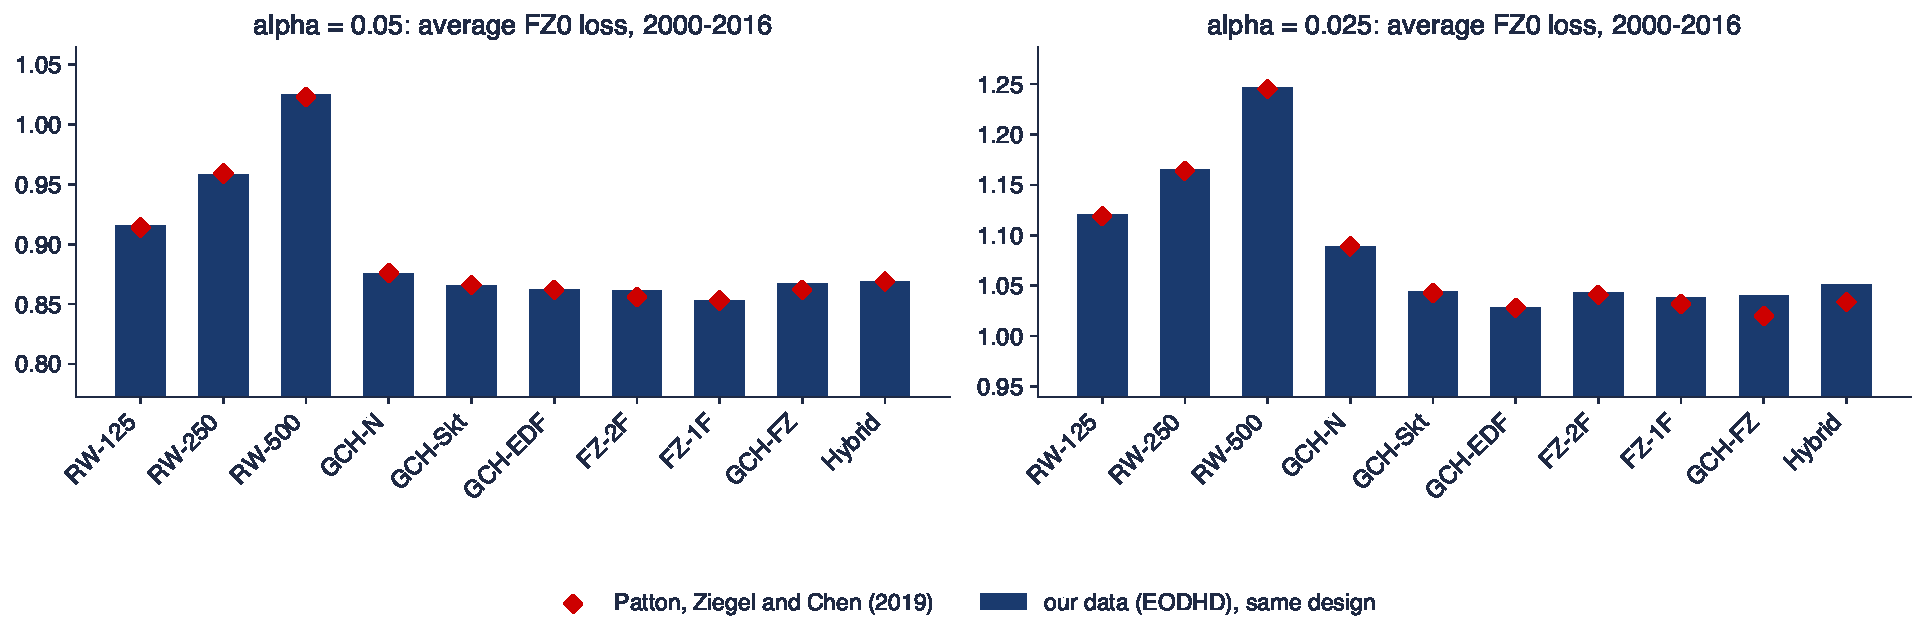
\includegraphics[width=0.97\textwidth,height=0.5\textheight,keepaspectratio]{ats_ch9_pzc_table.pdf}
\end{center}
\vspace{-0.25cm}
\begin{itemize}
    \item Pierderea FZ0 medie a zece modele (VaR, ES), S\&P 500, 2000--2016, designul \refPZC: datele noastre (bare), față de tabelul 8 al lucrării (romburi)
\end{itemize}
\quantlet{ATS\_ch9\_pzc}{https://github.com/danpele/Advanced-Time-Series/tree/main/Quantlets/Ch_09/ATS_ch9_pzc}
\end{frame}

\begin{frame}{Interpretarea celor două tipuri de rezultat}
\itemsize{\small}
\begin{itemize}
    \item Pierderile medii pe 4\,000 de zile sînt robuste la mici diferențe de date: GAS-1F 0{,}853, față de 0{,}853
    \item Testele care se bazează pe cîteva zeci de zile din coadă nu sînt: p-value-ul testului de adecvare 0{,}001, față de 0{,}242
    \item Același tipar în \atschlink{https://danpele.github.io/Advanced-Time-Series/RO/Cursuri/capitol2_rupturi_structurale_modele_neliniare.pdf}{Capitolul 2} (\refTPS: $p$ = 0{,}165, față de 0{,}002) și în \atschlink{https://danpele.github.io/Advanced-Time-Series/RO/Cursuri/capitol14_inferenta_cauzala_serii_timp.pdf}{Capitolul 14} (\refBMSS: $-$1{,}5\%, față de $-$2{,}4\%)
    \item Lecția: replicați separat estimația și inferența; raportați care dintre ele rezistă
\end{itemize}
\end{frame}

\begin{frame}{Cinci surse de diferențe}
\itemsize{\footnotesize}
\begin{itemize}
    \item \textbf{Ediția datelor}: PIB revizuit, indici de preț cu altă bază, serii care nu mai există
    \begin{itemize}
        \item diferența Brexit (\atschlink{https://danpele.github.io/Advanced-Time-Series/RO/Cursuri/capitol14_inferenta_cauzala_serii_timp.pdf}{Capitolul 14}), IPC-ul britanic din TPS (\atschlink{https://danpele.github.io/Advanced-Time-Series/RO/Cursuri/capitol2_rupturi_structurale_modele_neliniare.pdf}{Capitolul 2}), zecimalele MNZ (\atschlink{https://danpele.github.io/Advanced-Time-Series/RO/Cursuri/capitol6_modele_spatiul_starilor_filtrare_bayesiana.pdf}{Capitolul 6})
    \end{itemize}
    \item \textbf{Eșantionul}: efectul era o trăsătură a perioadei lui
    \begin{itemize}
        \item marja la termen (\atschlink{https://danpele.github.io/Advanced-Time-Series/RO/Cursuri/capitol0_recapitulare_inferenta.pdf}{Capitolul 0}), indicii de difuzie (\atschlink{https://danpele.github.io/Advanced-Time-Series/RO/Cursuri/capitol5_bvar_modele_factoriale_nowcasting.pdf}{Capitolul 5}), recesiunile lui Hamilton (\atschlink{https://danpele.github.io/Advanced-Time-Series/RO/Cursuri/capitol7_modele_schimbare_regim.pdf}{Capitolul 7})
    \end{itemize}
    \item \textbf{Implementarea}: optimizatorul, valorile de start, opțiunile implicite, cazul determinist
    \begin{itemize}
        \item maximele EM (\atschlink{https://danpele.github.io/Advanced-Time-Series/RO/Cursuri/capitol7_modele_schimbare_regim.pdf}{Capitolul 7}), rapoartele mari (\atschlink{https://danpele.github.io/Advanced-Time-Series/RO/Cursuri/capitol4_cointegrare_vecm_ardl_panel.pdf}{Capitolul 4}), inițializarea difuză (\atschlink{https://danpele.github.io/Advanced-Time-Series/RO/Cursuri/capitol6_modele_spatiul_starilor_filtrare_bayesiana.pdf}{Capitolul 6})
    \end{itemize}
    \item \textbf{Inferența}: estimația rezistă, eroarea standard sau valoarea critică nu
    \begin{itemize}
        \item fixed-$b$ (\atschlink{https://danpele.github.io/Advanced-Time-Series/RO/Cursuri/capitol0_recapitulare_inferenta.pdf}{Capitolul 0}), testele de adecvare (\atschlink{https://danpele.github.io/Advanced-Time-Series/RO/Cursuri/capitol9_var_es_backtesting.pdf}{Capitolul 9}), wild bootstrap (\atschlink{https://danpele.github.io/Advanced-Time-Series/RO/Cursuri/capitol16_radacini_explozive_bule_speculative.pdf}{Capitolul 16})
    \end{itemize}
    \item \textbf{Designul}: cadrul lucrării diferă de al dumneavoastră
    \begin{itemize}
        \item dimensiunea raportată la eșantion pentru DCC-NL (\atschlink{https://danpele.github.io/Advanced-Time-Series/RO/Cursuri/capitol8_volatilitate_avansata.pdf}{Capitolul 8}); funcția de pierdere pentru HARQ (\atschlink{https://danpele.github.io/Advanced-Time-Series/RO/Cursuri/capitol8_volatilitate_avansata.pdf}{Capitolul 8})
    \end{itemize}
\end{itemize}
\end{frame}

\begin{frame}{Replicarea corectă}
\itemsize{\small}
\begin{itemize}
    \item Obțineți pachetul de replicare; dacă nu există, notați fiecare alegere lăsată deschisă de lucrare
    \item Reproduceți întîi un singur rezultat (un coeficient, o statistică de test), apoi tabelul, apoi figura
    \item Păstrați eșantionul original ca rulare separată înainte de a-l extinde; schimbați un singur lucru odată
    \item Folosiți două implementări cînd este posibil (codul propriu și un pachet), ca pentru modelul lui Hamilton în \atschlink{https://danpele.github.io/Advanced-Time-Series/RO/Cursuri/capitol7_modele_schimbare_regim.pdf}{Capitolul 7}
    \item Puneți rezultatele publicate și cele replicate alături, cu diferențele absolute și relative
    \item O replicare nereușită este un rezultat: raportați sursa diferenței, testați explicațiile concurente, contactați politicos autorii dacă este nevoie
\end{itemize}
\end{frame}


%=============================================================================
\section{Lista de verificare a reproductibilității}
%=============================================================================

\begin{frame}{Repository-ul}
\itemsize{\small}
\begin{center}
\scriptsize
\begin{tabular}{>{\raggedright\arraybackslash}p{5.4cm}>{\raggedright\arraybackslash}p{6.8cm}}
\toprule
\textbf{Calea} & \textbf{Conținut} \\
\midrule
\texttt{README.md} & întrebarea, descrierea datelor, modul de rulare, durata \\
\texttt{requirements.txt} & versiunile pachetelor \\
\texttt{data/raw/}, \texttt{data/processed/} & fișierele brute nu se editează manual \\
\texttt{code/01\_data.py}, \texttt{02\_replication.py}, \dots & scripturi numerotate, rulate în ordine \\
\texttt{notebooks/main.ipynb} & rulează integral în Colab \\
\texttt{output/tables/}, \texttt{output/figures/} & generate de cod, niciodată scrise de mînă \\
\texttt{report/report.pdf} & articolul \\
\texttt{preregistration.md}, \texttt{AI\_USE.md}, \texttt{AI\_ERRORS.md} & planul și evidența folosirii AI \\
\bottomrule
\end{tabular}
\end{center}

\vspace{2mm}
\begin{itemize}
    \item Structura urmează cerințele editorilor de date ai revistelor de economie \refVil; pachetele de replicare sînt acum o condiție de publicare \refCM
    \item Fișierul preregistration.md este salvat (commit) înaintea primului commit cu estimări: istoricul o arată
\end{itemize}
\end{frame}

\begin{frame}{Lista de verificare a reproductibilității}
\itemsize{\small}
\begin{columns}[T]
\begin{column}{0.48\textwidth}
\begin{block}{Date și cod}
\begin{itemize}
    \item fiecare serie: sursa, codul, data descărcării
    \item niciun pas manual între datele brute și rezultate
    \item o singură comandă sau un singur notebook rulează totul
    \item seed-urile fixate și raportate; rezultatele stabile la schimbarea seed-ului
    \item funcțiile testate pe un caz cu răspuns cunoscut (un proces simulat, un rezultat publicat)
\end{itemize}
\end{block}
\end{column}
\begin{column}{0.48\textwidth}
\begin{block}{Rezultate și raport}
\begin{itemize}
    \item fiecare rezultat din raport provine dintr-un fișier din output/
    \item versiunile pachetelor în requirements.txt
    \item testul calculatorului curat: un coleg clonează repository-ul și obține aceleași rezultate \refPeng
    \item abaterile de la preînregistrare enumerate
    \item AI\_USE.md și AI\_ERRORS.md complete
\end{itemize}
\end{block}
\end{column}
\end{columns}
\end{frame}


%=============================================================================
\section{Erori frecvente}
%=============================================================================

\begin{frame}{Data snooping și p-hacking}
\itemsize{\small}
\begin{itemize}
    \item \textbf{Data snooping}: aceleași date se folosesc pentru a alege și pentru a testa un model; p-value-ul raportat ignoră căutarea \refWhite
    \begin{itemize}
        \item remedii: Reality Check, SPA \refHansen, StepM \refRW, MCS \refHLNa, o perioadă rezervată, neatinsă
    \end{itemize}
    \item \textbf{p-hacking}: flexibilitate nedeclarată (eșantioane, variabile de control, transformări, valori extreme) pînă cînd $p < 0{,}05$ \refSNS
    \begin{itemize}
        \item „grădina potecilor care se bifurcă”: nu este nevoie de o căutare conștientă, ajung alegerile dependente de date \refGL
        \item statisticile $z$ publicate se aglomerează imediat peste 1,96 \refBLSZ; în finanțe, un factor nou are nevoie de $t > 3$ \refHLZ
    \end{itemize}
    \item Predictorii persistenți adaugă o a doua problemă: testele HAC resping prea des, ca în \atschlink{https://danpele.github.io/Advanced-Time-Series/RO/Cursuri/capitol0_recapitulare_inferenta.pdf}{Capitolul 0} \refStam
\end{itemize}
\end{frame}

\begin{frame}{O căutare de specificații pe o serie fără predictibilitate}
\itemsize{\footnotesize}
\begin{center}
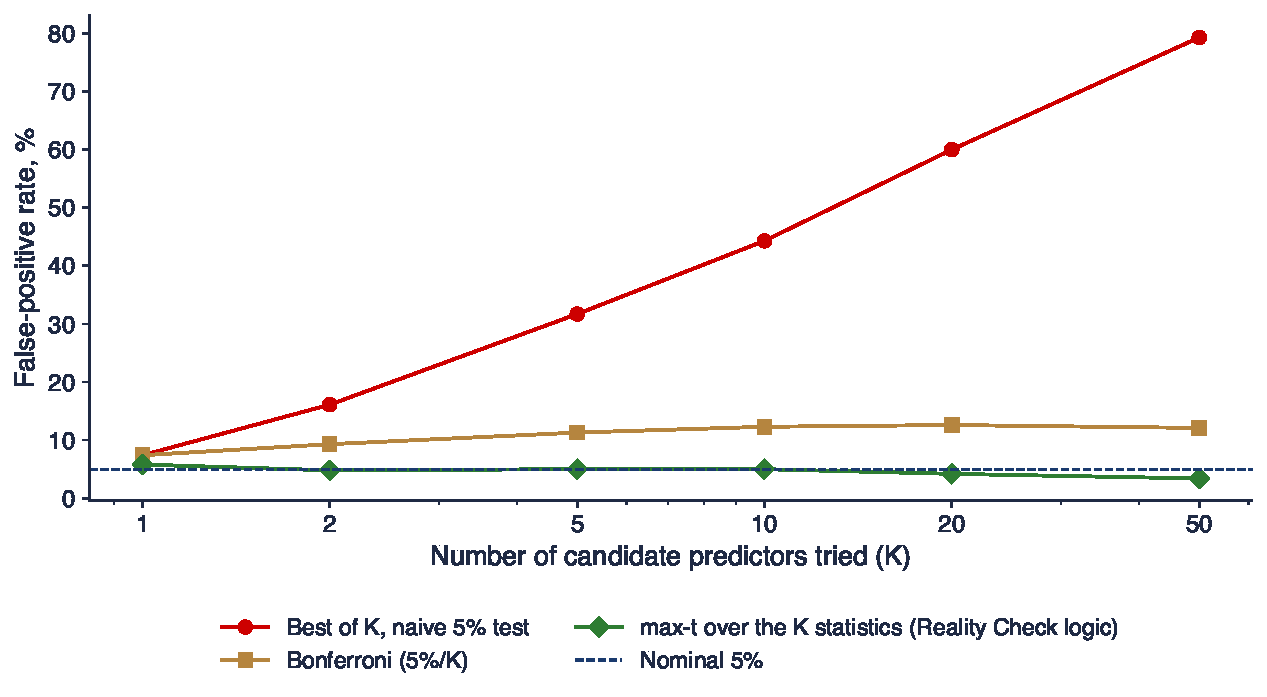
\includegraphics[width=0.97\textwidth,height=0.62\textheight,keepaspectratio]{ats_ch15_snooping.pdf}
\end{center}
\vspace{-0.25cm}
\begin{itemize}
    \item 1\,000 seturi de date simulate, $T$ = 250; $K$ predictori candidați persistenți ($\rho = 0{,}9$, un factor comun); teste $t$ HAC; proporția seturilor cu cel puțin o „descoperire”
\end{itemize}
\quantlet{ATS\_ch15\_pitfalls}{https://github.com/danpele/Advanced-Time-Series/tree/main/Quantlets/Ch_15/ATS_ch15_pitfalls}
\end{frame}

\begin{frame}{Interpretarea căutării de specificații}
\itemsize{\small}
\begin{itemize}
    \item Raportarea celui mai bun dintre $K$ ca și cum ar fi singurul încercat: 32\% rezultate fals pozitive cu 5 predictori, 60\% cu 20, 79\% cu 50
    \item Bonferroni nu rezolvă problema: 13\% la $K = 20$, pentru că fiecare test HAC este deja supradimensionat cu predictori persistenți (7\% la $K = 1$)
    \item Valoarea critică max-$t$ simulată sub ipoteza nulă, cu aceeași dependență, păstrează rata aproape de 5\%: 4\% la $K = 20$ (logica Reality Check)
    \item BET în \atschlink{https://danpele.github.io/Advanced-Time-Series/RO/Cursuri/capitol0_recapitulare_inferenta.pdf}{Capitolul 0}: $p$ naiv = 0{,}006, $p$ Reality Check = 0{,}06
    \item Preînregistrați $K$; raportați toate cele $K$ rezultate
\end{itemize}
\end{frame}

\begin{frame}{Leakage și look-ahead}
\itemsize{\small}
\begin{itemize}
    \item \textbf{Leakage}: informația din perioada de evaluare intră în model \refKau
    \begin{itemize}
        \item selecția predictorilor, a lagurilor sau a hiperparametrilor pe întregul eșantion
        \item scalare, eliminarea trendului, filtrare (HP, wavelet) sau imputare cu statistici din întregul eșantion
        \item K-fold aleator cu reziduuri dependente sau ținte suprapuse (\atschlink{https://danpele.github.io/Advanced-Time-Series/RO/Cursuri/capitol12_machine_learning_deep_learning.pdf}{Capitolul 12})
    \end{itemize}
    \item \textbf{Look-ahead}: folosirea datelor care nu erau disponibile la data prognozei
    \begin{itemize}
        \item date revizuite în locul edițiilor în timp real; întîrzierile de publicare ignorate
        \item modele preantrenate ale căror date de antrenare acoperă perioada de test (\atschlink{https://danpele.github.io/Advanced-Time-Series/RO/Cursuri/capitol13_foundation_models_conformal.pdf}{Capitolul 13})
    \end{itemize}
    \item Testul: aș fi putut calcula această prognoză la acea dată, cu acea informație?
\end{itemize}
\end{frame}

\begin{frame}{Selecția predictorilor cu look-ahead}
\itemsize{\footnotesize}
\begin{center}
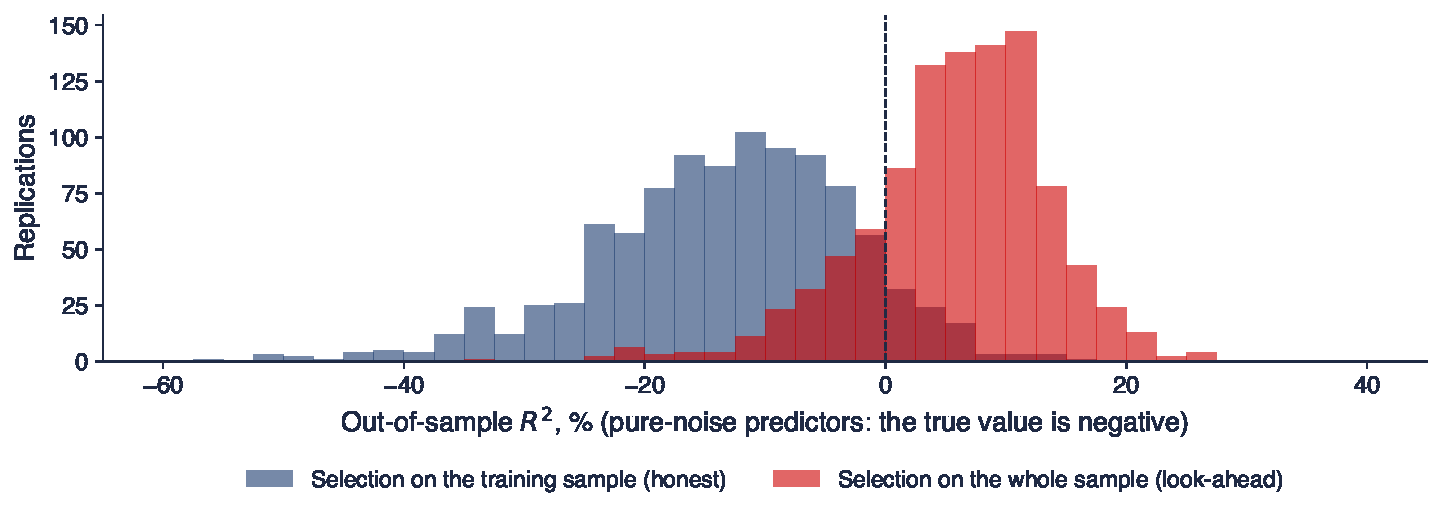
\includegraphics[width=0.97\textwidth,height=0.62\textheight,keepaspectratio]{ats_ch15_leakage.pdf}
\end{center}
\vspace{-0.25cm}
\begin{itemize}
    \item 1\,000 de simulări: $T$ = 240, ultimele 60 de perioade pentru test, 100 de predictori candidați de tip zgomot pur, se păstrează cei 5 mai corelați, MCO pe eșantionul de antrenare
\end{itemize}
\quantlet{ATS\_ch15\_pitfalls}{https://github.com/danpele/Advanced-Time-Series/tree/main/Quantlets/Ch_15/ATS_ch15_pitfalls}
\end{frame}

\begin{frame}{Interpretarea experimentului cu leakage}
\itemsize{\small}
\begin{itemize}
    \item Selecție corectă: $R^2$ mediu în afara eșantionului = \ensuremath{-}13{,}3\%, pozitiv în 8\% din rulări: zgomotul nu prognozează
    \item Selecție pe întregul eșantion: media 5{,}9\%, pozitiv în 81\% din rulări: un „cîștig de prognoză” creat chiar de perioada de test
    \item Evaluarea în afara eșantionului vă protejează doar dacă fiecare alegere se face în fereastra de antrenare \refIK
    \item Același mecanism a supraestimat scorurile de validare din \atschlink{https://danpele.github.io/Advanced-Time-Series/RO/Cursuri/capitol12_machine_learning_deep_learning.pdf}{Capitolul 12} (raport 0{,}34)
\end{itemize}
\end{frame}

\begin{frame}{Afirmații exagerate}
\itemsize{\footnotesize}
\begin{columns}[T]
\begin{column}{0.58\textwidth}
\begin{itemize}
    \item \textbf{Limbaj cauzal pentru rezultate predictive}
    \begin{itemize}
        \item „cauzează în sens Granger” nu înseamnă „cauzează”; un factor comun sau momentul observării o produc (\atschlink{https://danpele.github.io/Advanced-Time-Series/RO/Cursuri/capitol14_inferenta_cauzala_serii_timp.pdf}{Capitolul 14})
    \end{itemize}
    \item \textbf{Semnificația în locul mărimii}
    \begin{itemize}
        \item un test DM semnificativ cu o reducere a pierderii de 0,3\% este un cîștig mic; raportați efectul și intervalul lui
    \end{itemize}
    \item \textbf{Generalitate pe baza unui singur eșantion}
    \begin{itemize}
        \item o piață, o perioadă, o specificație; spuneți-o în titlu și în rezumat
    \end{itemize}
    \item \textbf{Absența dovezii drept dovadă a absenței}
    \begin{itemize}
        \item o nerespingere cu putere mică spune puțin: calculați puterea (nowcast-ul României, $p$ = 0{,}76)
    \end{itemize}
\end{itemize}
\end{column}
\begin{column}{0.38\textwidth}
\centering
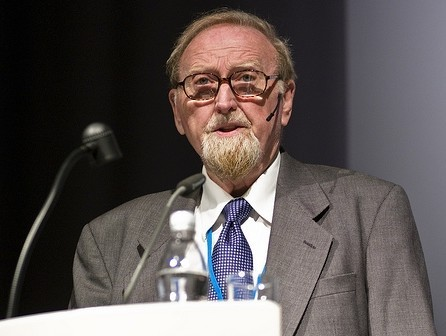
\includegraphics[height=0.40\textheight]{ch1_granger_2008.jpg}\\[1mm]
\imgcap{Clive Granger (2008)}
\imgcredit{https://commons.wikimedia.org/wiki/File:Clive_Granger_by_Olaf_Storbeck.jpg}{Foto: Olaf Storbeck (2008); CC BY-SA 2.0; Wikimedia Commons}
\end{column}
\end{columns}
\end{frame}

\begin{frame}{Recapitulare: erorile frecvente}
\itemsize{\small}
\begin{itemize}
    \item O căutare raportată ca un singur test produce descoperiri din zgomot; preînregistrați $K$ și corectați
    \item Fiecare alegere în fereastra de antrenare, fiecare dată disponibilă la data prognozei
    \item Afirmații nu mai puternice decît designul: predicția nu este cauzalitate, semnificația nu este mărime
\end{itemize}
\end{frame}


%=============================================================================
\section{Susținerea orală}
%=============================================================================

\begin{frame}{Formatul susținerii}
\itemsize{\small}
\begin{columns}[T]
\begin{column}{0.6\textwidth}
\begin{itemize}
    \item Individuală, circa 15 minute pentru fiecare student: fiecare membru este examinat separat și primește o notă separată (50\% din nota finală)
    \item 5 minute: prezentarea contribuției proprii, adică a părții de proiect coordonate de student, pe baza raportului și a repository-ului
    \item 10 minute: întrebări despre cod, metodă și rezultate
    \begin{itemize}
        \item codul: deschideți un fișier, explicați o funcție, spuneți ce se schimbă dacă se schimbă o alegere
        \item metoda: teoria din spatele ei, ipotezele și alternativele
        \item rezultatele: interpretați un rezultat, un test, o figură; apărați inferența
    \end{itemize}
    \item Se notează după criteriile de pe slide-ul următor
    \item Fiecare membru trebuie să poată răspunde la întrebări despre întregul proiect, nu doar despre partea proprie
    \item Fără instrumente AI în timpul susținerii; în română sau în engleză
\end{itemize}
\end{column}
\begin{column}{0.36\textwidth}
\centering
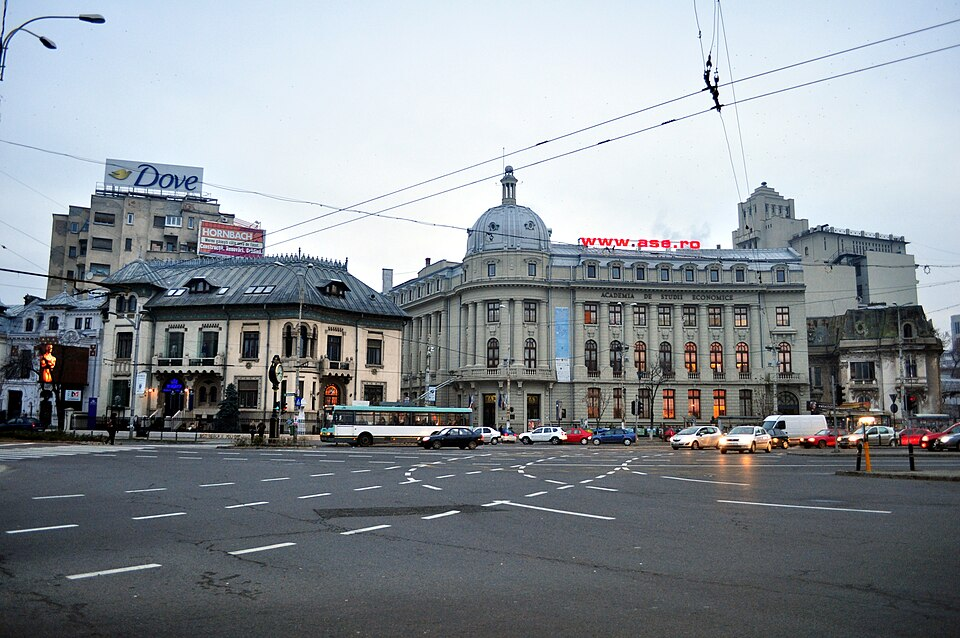
\includegraphics[height=0.36\textheight]{ch0_ase_2014.jpg}\\[1mm]
\imgcap{Academia de Studii Economice din București}
\imgcredit{https://commons.wikimedia.org/wiki/File:Bucharest_-_Academie_de_Studii_Economice_01.jpg}{Foto: Joe Mabel (2014); CC BY 3.0; Wikimedia Commons}
\end{column}
\end{columns}
\end{frame}

\begin{frame}{Criteriile de evaluare a susținerii individuale}
\itemsize{\small}
\begin{center}
\scriptsize
\begin{tabular}{>{\raggedright\arraybackslash}p{3.4cm}>{\raggedright\arraybackslash}p{1.1cm}>{\raggedright\arraybackslash}p{8.2cm}}
\toprule
\textbf{Criteriul} & \textbf{Puncte} & \textbf{Ce aduce punctele} \\
\midrule
Stăpînirea metodei & 25 & formulează modelul și ipotezele, derivă rezultatul-cheie, știe cînd metoda nu funcționează \\
Stăpînirea codului și a datelor & 20 & explică orice funcție din repository, sursa și ediția datelor, efectul schimbării unei setări \\
Inferența și interpretarea & 25 & erori standard valide pentru date dependente, mărimi ale efectelor cu intervale, citirea corectă a testelor și a nerespingerilor \\
Replicarea și robustețea & 20 & explică diferențele față de lucrare, designul de robustețe și limitele concluziei \\
Integritatea cercetării și folosirea AI & 10 & descrie ce a făcut AI, ce erori au fost depistate și cum; abaterile de la preînregistrare \\
\bottomrule
\end{tabular}
\end{center}
\begin{itemize}
    \item Nota la susținere este punctajul din 100 împărțit la 10; un membru care nu poate explica codul predat nu poate promova
\end{itemize}
\end{frame}

\begin{frame}{Criteriile care diferențiază notele}
\itemsize{\small}
\begin{itemize}
    \item \textbf{9--10}
    \begin{itemize}
        \item răspunde la „de ce” și „ce s-ar întîmpla dacă”, nu doar la „ce”; anticipează punctele slabe și le-a testat
    \end{itemize}
    \item \textbf{7--8}
    \begin{itemize}
        \item metode și interpretare corecte; ezită la alternative sau la asimptotică
    \end{itemize}
    \item \textbf{5--6}
    \begin{itemize}
        \item poate rula și descrie codul; citește mecanic p-value-urile; legătură limitată cu teoria
    \end{itemize}
    \item \textbf{sub 5}
    \begin{itemize}
        \item nu poate explica propriul cod sau propriile rezultate; afirmații nesusținute de rezultate; folosire nedeclarată a AI
    \end{itemize}
\end{itemize}
\end{frame}

\begin{frame}{Întrebări tipice cu răspunsuri-model (1/3): codul}
\itemsize{\footnotesize}
\begin{itemize}
    \item \textbf{Î}: Unde se fixează în codul dumneavoastră mulțimea de informație a prognozei pentru data $t$?
    \begin{itemize}
        \item \textbf{Răspuns-model}: În bucla walk-forward: fereastra de estimare se termină la $t - h$, iar scalarea, selecția și calibrarea hiperparametrilor se recalculează în buclă (arată liniile)
    \end{itemize}
    \item \textbf{Î}: Cîte laguri HAC folosiți și de ce?
    \begin{itemize}
        \item \textbf{Răspuns-model}: Regula Newey--West $\lfloor 4(T/100)^{2/9}\rfloor$ ($T$: mărimea eșantionului; $\lfloor\cdot\rfloor$: partea întreagă), cel puțin $h - 1$ pentru erori suprapuse la $h$ pași; verificat cu valori critice fixed-$b$ (\atschlink{https://danpele.github.io/Advanced-Time-Series/RO/Cursuri/capitol0_recapitulare_inferenta.pdf}{Capitolul 0})
    \end{itemize}
    \item \textbf{Î}: Ce se întîmplă dacă schimbați seed-ul?
    \begin{itemize}
        \item \textbf{Răspuns-model}: Am rulat din nou cu zece seed-uri: ierarhia nu se schimbă, pierderea variază cu mai puțin decît eroarea ei standard (un tabel în raport)
    \end{itemize}
\end{itemize}
\end{frame}

\begin{frame}{Întrebări tipice cu răspunsuri-model (2/3): rezultatele}
\itemsize{\footnotesize}
\begin{itemize}
    \item \textbf{Î}: Testul DM dă $p = 0{,}03$: este modelul dumneavoastră mai bun?
    \begin{itemize}
        \item \textbf{Răspuns-model}: Mai bun pentru funcția de pierdere preînregistrată, pe acest eșantion: diferența medie a pierderilor este X, cu un interval HAC; modelele nu sînt imbricate, deci DM este valid; pentru mai multe modele raportăm MCS
    \end{itemize}
    \item \textbf{Î}: Replicarea diferă de tabelul 2 din lucrare. De ce?
    \begin{itemize}
        \item \textbf{Răspuns-model}: Pe eșantionul original coincidem la două zecimale; diferența apare cu ediția actuală a datelor, deci este revizuire, nu cod (arată cele două rulări)
    \end{itemize}
    \item \textbf{Î}: Ce rezultat v-ar fi făcut să respingeți ipoteza?
    \begin{itemize}
        \item \textbf{Răspuns-model}: Preînregistrarea o spune: o dată placebo cu un efect asemănător sau un efect care își schimbă semnul între grupurile de donatori
    \end{itemize}
\end{itemize}
\end{frame}

\begin{frame}{Întrebări tipice cu răspunsuri-model (3/3): capitolele}
\itemsize{\footnotesize}
\begin{itemize}
    \item \textbf{Î}: De ce nu puteți folosi valori critice $\chi^2$ pentru a testa două regimuri față de unul?
    \begin{itemize}
        \item \textbf{Răspuns-model}: Sub ipoteza nulă, probabilitățile de tranziție nu sînt identificate, un parametru este la limită și scorul este zero: este nevoie de bootstrap sau de metodele lui Hansen și Garcia (\atschlink{https://danpele.github.io/Advanced-Time-Series/RO/Cursuri/capitol7_modele_schimbare_regim.pdf}{Capitolul 7})
    \end{itemize}
    \item \textbf{Î}: De ce este acceptabilă validarea K-fold pentru modelul AR, dar nu pentru random forest?
    \begin{itemize}
        \item \textbf{Răspuns-model}: Pentru o autoregresie bine specificată reziduurile sînt necorelate, deci partițiile sînt valide \refBHK; reziduurile random forest sînt autocorelate, deci folosim blocuri și purjare (\atschlink{https://danpele.github.io/Advanced-Time-Series/RO/Cursuri/capitol12_machine_learning_deep_learning.pdf}{Capitolul 12})
    \end{itemize}
    \item \textbf{Î}: Este un test Granger semnificativ un efect cauzal?
    \begin{itemize}
        \item \textbf{Răspuns-model}: Nu: este predictiv, relativ la o mulțime de informație; o afirmație cauzală cere o ipoteză de identificare despre alocare, de exemplu un instrument sau un control sintetic cu placebo (\atschlink{https://danpele.github.io/Advanced-Time-Series/RO/Cursuri/capitol14_inferenta_cauzala_serii_timp.pdf}{Capitolul 14})
    \end{itemize}
\end{itemize}
\end{frame}

\begin{frame}{Unde greșesc susținerile}
\itemsize{\small}
\begin{itemize}
    \item Cod scris de altcineva (un coleg sau un asistent AI) pe care cel care prezintă nu îl poate explica
    \item Un p-value citit drept probabilitatea ca ipoteza să fie adevărată
    \item Un cîștig de prognoză fără test sau un test fără mărimea cîștigului
    \item Necunoașterea datelor: sursa, frecvența, ediția, transformările, datele eșantionului
    \item Rezultate din raport pe care repository-ul nu le reproduce
    \item Apărarea fiecărui rezultat în loc de explicarea limitelor lui
\end{itemize}
\end{frame}


%=============================================================================
\section{AI în cercetare}
%=============================================================================

\begin{frame}{AI\_USE.md: ce s-a cerut și ce s-a păstrat}
\itemsize{\small}
\begin{itemize}
    \item Instrumentele AI sînt permise și se declară; folosirea nedeclarată este considerată plagiat
    \item Pentru fiecare folosire, o intrare
    \begin{itemize}
        \item instrumentul și versiunea, data, etapa din fluxul de cercetare
        \item promptul (sau un rezumat fidel al lui)
        \item ce s-a păstrat, ce s-a modificat sau respins și cum s-a verificat
    \end{itemize}
    \item Folosiri utile
    \begin{itemize}
        \item căutarea literaturii cu DOI verificate; prime variante de cod, cu teste; critica designului în rolul unui recenzent ostil \refKor
    \end{itemize}
    \item Folosiri riscante
    \begin{itemize}
        \item referințe, rezultate și date preluate fără verificare \refWW; text care afirmă mai mult decît rezultatele
        \item iluzia înțelegerii: un text fluent confundat cu cunoașterea \refMC
    \end{itemize}
\end{itemize}
\end{frame}

\begin{frame}{AI\_ERRORS.md: cel puțin trei erori depistate}
\itemsize{\small}
\begin{center}
\scriptsize
\begin{tabular}{>{\raggedright\arraybackslash}p{2.6cm}>{\raggedright\arraybackslash}p{5.0cm}>{\raggedright\arraybackslash}p{4.8cm}}
\toprule
\textbf{Tipul} & \textbf{Exemplu din curs} & \textbf{Cum se depistează} \\
\midrule
referință inventată & un titlu plauzibil cu un DOI care duce la altă lucrare & căutare în Crossref: titlul și autorii trebuie să coincidă \\
formulă greșită & ES evaluat singur cu o pierdere de cuantilă (\atschlink{https://danpele.github.io/Advanced-Time-Series/RO/Cursuri/capitol9_var_es_backtesting.pdf}{Capitolul 9}) & derivare pe hîrtie; o simulare cu răspuns cunoscut \\
leakage în cod & o scalare estimată pe întregul eșantion înainte de împărțire & testul datei: recalculați o prognoză doar cu datele de pînă la data ei \\
opțiune implicită greșită & o valoare critică $\chi^2$ pentru un test sup (\atschlink{https://danpele.github.io/Advanced-Time-Series/RO/Cursuri/capitol2_rupturi_structurale_modele_neliniare.pdf}{Capitolul 2}) & citiți documentația și lucrarea; reproduceți o valoare publicată \\
afirmație exagerată & „cauzalitatea Granger dovedește că ...” (\atschlink{https://danpele.github.io/Advanced-Time-Series/RO/Cursuri/capitol14_inferenta_cauzala_serii_timp.pdf}{Capitolul 14}) & comparați fiecare frază cu designul \\
\bottomrule
\end{tabular}
\end{center}
\begin{itemize}
    \item Fiecare intrare: ce a produs instrumentul, de ce era greșit, cum a fost depistat, ce l-a înlocuit
\end{itemize}
\end{frame}

\begin{frame}{Un protocol de verificare}
\itemsize{\small}
\begin{itemize}
    \item Referințele: fiecare DOI verificat și titlul confirmat; rezultatul invocat găsit în lucrare
    \item Codul: rulat pe un proces simulat cu parametri cunoscuți înainte de datele reale; comparat cu o a doua implementare
    \item Rezultatele: fiecare rezultat din raport regenerat de repository; niciunul copiat dintr-o conversație
    \item Datele calendaristice și faptele: din surse oficiale (Eurostat, BNR, Monitorul Oficial), nu din memoria modelului
    \item Textul: fiecare afirmație verificată față de design (predicție, asociere sau cauzalitate)
    \item La susținere explicați totul singur: ce nu puteți explica nu ar trebui să fie în proiect
\end{itemize}
\end{frame}


%=============================================================================
\section{AI în descoperirea științifică: alegerea proiectului}
%=============================================================================

\begin{frame}{Întrebarea deschisă}
\itemsize{\small}
\begin{itemize}
    \item \textbf{Ce rezultate de referință din econometria seriilor de timp rezistă pe date noi și de ce unele nu?}
    \begin{itemize}
        \item replicările din curs indică edițiile datelor, eșantioanele și inferența; un răspuns sistematic, pentru mai multe lucrări, nu există
    \end{itemize}
    \item Instrumentele AI schimbă costul fiecărei etape
    \begin{itemize}
        \item hărți ale literaturii și variante de cod în cîteva ore \refWang; s-au propus fluxuri complet automatizate \refLu
        \item resursa rară devine judecata: designul, verificările, interpretarea
    \end{itemize}
    \item Proiectul dumneavoastră este un punct de date pentru această întrebare: o replicare cu un verdict clar și un motiv documentat
\end{itemize}
\end{frame}

\begin{frame}{Bucla de cercetare cu un asistent AI}
\itemsize{\footnotesize}
\begin{itemize}
    \item Un asistent AI (un LLM precum Claude, ChatGPT, Gemini sau Copilot) accelerează fiecare etapă; Semantic Scholar și Elicit ajută la literatură
    \begin{itemize}
        \item \textbf{literatura}: \aiprompt{Listează replicările lucrării Meese și Rogoff (1983) pentru monedele din Europa Centrală și de Est din 2010 încoace, cu DOI, orizonturi și verdicte.} Apoi verificați fiecare DOI
        \item \textbf{designul}: \aiprompt{Pentru o diferență a pierderilor cu autocorelația 0,3, cîte luni în afara eșantionului sînt necesare pentru o putere de 80\% la detectarea unui cîștig mediu de 0,2 abateri standard?}
        \item \textbf{cod și replicare}: cereți o funcție DM--HLN, apoi testați-o pe date simulate cu răspuns cunoscut
        \item \textbf{critica}: \aiprompt{Joacă rolul unui recenzent ostil al acestei preînregistrări: unde pot rezultatele să influențeze designul?}
    \end{itemize}
    \item Raportul: ce s-a cerut, ce s-a păstrat, ce s-a respins (AI\_USE.md, AI\_ERRORS.md)
\end{itemize}
\end{frame}

\begin{frame}{Verificări necesare}
\itemsize{\small}
\begin{itemize}
    \item Lucrarea există, spune ce se afirmă, iar datele ei sînt disponibile azi
    \item Calculul puterii folosește dependența propriei diferențe a pierderilor, estimată pe perioada de antrenare
    \item Formula din spatele unui răspuns AI: o afirmație despre putere fără varianța de termen lung este greșită pentru date dependente
    \item Extensia este realizabilă într-un semestru cu instrumentele cursului
    \item Criteriile verdictului (replicat, parțial, nereplicat) sînt scrise înainte de a rula replicarea
\end{itemize}
\end{frame}

\begin{frame}{Mini studiu de caz: este eșantionul de evaluare destul de lung?}
\itemsize{\footnotesize}
\begin{center}
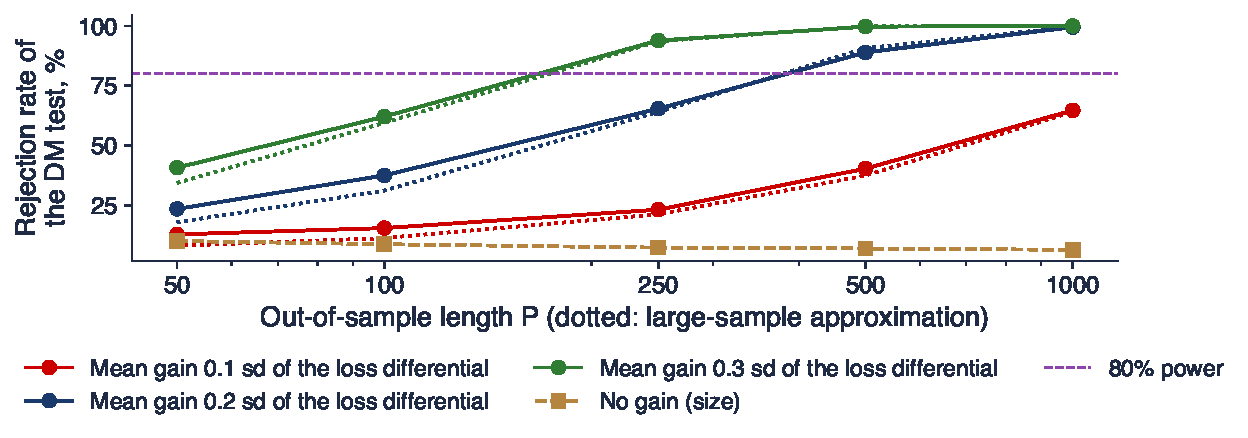
\includegraphics[width=0.97\textwidth,height=0.56\textheight,keepaspectratio]{ats_ch15_power.pdf}
\end{center}
\vspace{-0.25cm}
\begin{itemize}
    \item Rata de respingere a testului DM--HLN (5\%, bilateral, 2\,000 de simulări) cînd diferența pierderilor este un cîștig mediu $\delta$ plus un zgomot AR(1) cu coeficientul $\rho = 0{,}3$ și varianța 1
    \item Punctat: aproximarea $\Phi\big(\delta\sqrt{P/\Omega} - 1{,}96\big)$; $\Phi$: funcția de repartiție a distribuției Normale standard; $P$: numărul de observații în afara eșantionului; $\Omega$: varianța de termen lung a diferenței
\end{itemize}
\quantlet{ATS\_ch15\_power}{https://github.com/danpele/Advanced-Time-Series/tree/main/Quantlets/Ch_15/ATS_ch15_power}
\end{frame}

\begin{frame}{Interpretarea mini studiului de caz}
\itemsize{\small}
\begin{itemize}
    \item Un cîștig de 0,2 abateri standard este detectat cu probabilitatea 38\% la $P = 100$ și 89\% la $P = 500$; o putere de 80\% cere aproximativ 364 de observații
    \item Un cîștig de 0,1 cere aproximativ 1458: mai mult de 120 de ani de date lunare; un cîștig de 0,3 aproximativ 162
    \item Regula de mărime a eșantionului $P \approx \Omega\,(z_{0{,}975} + z_{0{,}8})^2/\delta^2$, cu $\Omega = (1 + \rho)/(1 - \rho)$ = 1{,}86: dependența multiplică eșantionul necesar
    \begin{itemize}
        \item $z_{0{,}975} = 1{,}96$, $z_{0{,}8} = 0{,}84$: cuantilele distribuției Normale pentru un test bilateral de 5\% și o putere de 80\%; $\delta$: cîștigul mediu, în abateri standard
    \end{itemize}
    \item Cu puține observații testul este și supradimensionat: 10{,}1\% la $P = 50$
    \item Alegeți o întrebare la care datele pot răspunde: datele macro lunare detectează rar cîștiguri mici, datele zilnice sau intrazilnice pot
\end{itemize}
\end{frame}

\begin{frame}{Idee de proiect}
\itemsize{\small}
\begin{itemize}
    \item \textbf{Alegerea proiectului: patru criterii}
    \begin{itemize}
        \item o lucrare de referință cu date publice sau o descriere precisă a datelor și un rezultat de reprodus
        \item o extensie care răspunde unei întrebări noi, de preferință pe date din România sau din UE
        \item suficientă putere pentru evaluarea planificată (mini studiul de caz)
        \item o regulă a verdictului scrisă înaintea primei estimări
    \end{itemize}
    \item \textbf{Exemplu}: de ce eșuează unele replicări? Un audit de replicare pentru trei lucrări din curs
    \begin{itemize}
        \item replicați \refTPS, \refPZC{} și \refBMSS{} pe datele originale și pe cele de azi; atribuiți fiecare diferență ediției, eșantionului, implementării sau inferenței
        \item extindeți: ediții arhivate ale datelor (ALFRED, OECD Economic Outlook), o curbă a specificațiilor, o analiză a puterii fiecărui test original
    \end{itemize}
    \item Livrabilele urmează regulile cursului: repository, raport, AI\_USE.md, AI\_ERRORS.md, susținere orală
\end{itemize}
\end{frame}


%=============================================================================
\section{Încheiere}
%=============================================================================

\begin{frame}{Idei de reținut}
\itemsize{\small}
\begin{itemize}
    \item Cinci întrebări pentru orice analiză: ținta, dependența, identificarea, evaluarea, robustețea
    \item Majoritatea rezultatelor de referință se replică în sens; mărimea și testele lor depind de ediția datelor, de eșantion și de inferență
    \item Preînregistrați designul, calculați puterea și faceți fiecare rezultat reproductibil dintr-o singură comandă
    \item Căutările, leakage-ul și look-ahead creează descoperiri din zgomot; cuvintele cauzale cer designuri cauzale
    \item Susținerea este individuală: explicați singur metoda, codul, inferența și limitele
\end{itemize}
\end{frame}

\begin{frame}{Autoevaluare}
\itemsize{\small}
\begin{columns}[T]
\begin{column}{0.58\textwidth}
\begin{block}{Întrebări}
\begin{itemize}
    \item Ce ipoteză identifică rezultatul principal al proiectului dumneavoastră?
    \item Cîte specificații ați încercat și cum ține cont inferența dumneavoastră de ele?
    \item Ar fi putut fi calculată fiecare prognoză la data ei?
    \item Care este puterea testului principal?
    \item Care dintre rezultatele dumneavoastră s-ar schimba cu o nouă ediție a datelor?
\end{itemize}
\end{block}
\end{column}
\begin{column}{0.38\textwidth}
\begin{block}{Studiu suplimentar}
\begin{itemize}
    \item \refCM; \refCle; \refMen
    \item \refDiebold; \refLLSW
    \item \atschlink{https://danpele.github.io/Advanced-Time-Series/RO/Cursuri/capitol16_radacini_explozive_bule_speculative.pdf}{Capitolul 16} (studiu individual) și quiz-ul lui
\end{itemize}
\end{block}
\end{column}
\end{columns}
\end{frame}


%=============================================================================
\section{Anexă}
%=============================================================================

\begin{frame}{Anexă: idei de proiect pe capitole (1/2)}
\hypertarget{atsapp1}{}\atsappback{atssrc1}{Înapoi}
\itemsize{\small}
\begin{center}
\scriptsize
\begin{tabular}{l>{\raggedright\arraybackslash}p{5.0cm}>{\raggedright\arraybackslash}p{6.6cm}}
\toprule
\textbf{Cap.} & \textbf{Replicați} & \textbf{Extindeți} \\
\midrule
0 & \refEH{} & zona euro și România; inferență fixed-$b$; stabilitatea pe decenii \\
1 & \refMR{} & monedele din ECE, prognoze de densitate, fundamente macro în timp real \\
2 & \refBP{} & rupturi în inflația României și în dobînda de politică monetară; monitorizare în timp real \\
3 & \refGK{} & surprizele BCE și condițiile financiare din România cu LP-IV \\
4 & \refPSS{} & transmiterea dobînzilor în UE cu CCE \\
5 & \refBGR{} & un BVAR mare cu volatilitate stochastică pentru România, nowcasting cu știri \\
6 & \refMNZ{} & output gap-ul României și revizuirile lui în timp real \\
7 & \refHam{} & probabilități de recesiune în timp real pentru zona euro \\
8 & \refBPQ{} & HARQ pentru BET și EUR/RON cu măsuri realizate \\
\bottomrule
\end{tabular}
\end{center}
\end{frame}

\begin{frame}{Anexă: idei de proiect pe capitole (2/2)}
\hypertarget{atsapp2}{}\atsappback{atssrc1}{Înapoi}
\itemsize{\small}
\begin{center}
\scriptsize
\begin{tabular}{l>{\raggedright\arraybackslash}p{5.0cm}>{\raggedright\arraybackslash}p{6.6cm}}
\toprule
\textbf{Cap.} & \textbf{Replicați} & \textbf{Extindeți} \\
\midrule
9 & \refPZC{} & indicii din ECE; puterea backtest-urilor \\
10 & \refGJR{} & caracterul rough al volatilității în ECE și pe cripto; robustețea la zgomot \\
11 & \refCN, \refHamB{} & output gap-uri în timp real pentru statele membre UE \\
12 & \refZeng{} & consumul de electricitate din UE; modele globale; comparații oneste \\
13 & \refGC{} & VaR conformal pentru BET; acoperire pe regimuri \\
14 & \refADH, \refBMSS{} & măsuri fiscale și energetice în ECE cu controale sintetice \\
16 & \refPY{} & prețurile și chiriile locuințelor în capitalele UE \\
15 & \refTPS, \refPZC, \refBMSS{} & un audit de replicare (ideea de proiect a acestui capitol) \\
\bottomrule
\end{tabular}
\end{center}
\begin{itemize}
    \item Partea C a fiecărui seminar conține încă o idee de proiect, cu datele ei
\end{itemize}
\end{frame}

\begin{frame}{Anexă: un model de preînregistrare}
\hypertarget{atsapp3}{}\atsappback{atssrc1}{Înapoi}
\itemsize{\small}
\begin{itemize}
    \item \textbf{1. Întrebarea și ipotezele}: ipoteza principală, într-o frază; ipotezele secundare
    \item \textbf{2. Lucrarea replicată}: tabelul sau figura, eșantionul, ce înseamnă „replicat”, „parțial”, „nereplicat”
    \item \textbf{3. Datele}: seriile, sursele, data ediției, frecvența, transformările, excluderile
    \item \textbf{4. Modelele}: reperul și modelele concurente, metoda de estimare, alegerea hiperparametrilor (în fereastra de antrenare)
    \item \textbf{5. Evaluarea}: ferestrele (mobile sau extinse), orizonturile, funcțiile de pierdere, testele, corecția pentru testarea multiplă, calculul puterii
    \item \textbf{6. Robustețea}: lista variațiilor și regula pentru un rezultat robust
    \item \textbf{7. Echipa}: cine coordonează fiecare parte (baza susținerii individuale)
\end{itemize}
\end{frame}


%=============================================================================
\section{Bibliografie}
%=============================================================================

\begin{frame}{Bibliografie (1/6)}
\itemsize{\tiny}
\begin{itemize}
    \item Abadie, A., Diamond, A., \& Hainmueller, J. (2015). Comparative politics and the synthetic control method. \textit{American Journal of Political Science}, 59(2), 495--510. \href{https://doi.org/10.1111/ajps.12116}{doi:10.1111/ajps.12116}
    \item Atkeson, A., \& Ohanian, L. E. (2001). Are Phillips curves useful for forecasting inflation? \textit{Federal Reserve Bank of Minneapolis Quarterly Review}, 25(1), 2--11. \href{https://doi.org/10.21034/qr.2511}{doi:10.21034/qr.2511}
    \item Bańbura, M., Giannone, D., \& Reichlin, L. (2010). Large Bayesian vector auto regressions. \textit{Journal of Applied Econometrics}, 25(1), 71--92. \href{https://doi.org/10.1002/jae.1137}{doi:10.1002/jae.1137}
    \item Bai, J., \& Perron, P. (2003). Computation and analysis of multiple structural change models. \textit{Journal of Applied Econometrics}, 18(1), 1--22. \href{https://doi.org/10.1002/jae.659}{doi:10.1002/jae.659}
    \item Bergmeir, C., Hyndman, R. J., \& Koo, B. (2018). A note on the validity of cross-validation for evaluating autoregressive time series prediction. \textit{Computational Statistics \& Data Analysis}, 120, 70--83. \href{https://doi.org/10.1016/j.csda.2017.11.003}{doi:10.1016/j.csda.2017.11.003}
    \item Bollerslev, T., Patton, A. J., \& Quaedvlieg, R. (2016). Exploiting the errors: A simple approach for improved volatility forecasting. \textit{Journal of Econometrics}, 192(1), 1--18. \href{https://doi.org/10.1016/j.jeconom.2015.10.007}{doi:10.1016/j.jeconom.2015.10.007}
    \item Born, B., Müller, G. J., Schularick, M., \& Sedláček, P. (2019). The costs of economic nationalism: Evidence from the Brexit experiment. \textit{The Economic Journal}, 129(623), 2722--2744. \href{https://doi.org/10.1093/ej/uez020}{doi:10.1093/ej/uez020}
    \item Brodeur, A., Lé, M., Sangnier, M., \& Zylberberg, Y. (2016). Star wars: The empirics strike back. \textit{American Economic Journal: Applied Economics}, 8(1), 1--32. \href{https://doi.org/10.1257/app.20150044}{doi:10.1257/app.20150044}
    \item Chang, A. C., \& Li, P. (2022). Is economics research replicable? Sixty published papers from thirteen journals say ``often not''. \textit{Critical Finance Review}, 11(1), 185--206. \href{https://doi.org/10.1561/104.00000053}{doi:10.1561/104.00000053}
    \item Christensen, G., \& Miguel, E. (2018). Transparency, reproducibility, and the credibility of economics research. \textit{Journal of Economic Literature}, 56(3), 920--980. \href{https://doi.org/10.1257/jel.20171350}{doi:10.1257/jel.20171350}
    \item Christiano, L. J., Eichenbaum, M., \& Evans, C. L. (1999). Monetary policy shocks: What have we learned and to what end? In J. B. Taylor \& M. Woodford (Eds.), \textit{Handbook of Macroeconomics}, Vol.\ 1A, 65--148. Elsevier. \href{https://doi.org/10.1016/S1574-0048(99)01005-8}{doi:10.1016/S1574-0048(99)01005-8}
    \item Clark, T. E., \& West, K. D. (2007). Approximately normal tests for equal predictive accuracy in nested models. \textit{Journal of Econometrics}, 138(1), 291--311. \href{https://doi.org/10.1016/j.jeconom.2006.05.023}{doi:10.1016/j.jeconom.2006.05.023}
    \item Clemens, M. A. (2017). The meaning of failed replications: A review and proposal. \textit{Journal of Economic Surveys}, 31(1), 326--342. \href{https://doi.org/10.1111/joes.12139}{doi:10.1111/joes.12139}
\end{itemize}
\end{frame}

\begin{frame}{Bibliografie (2/6)}
\itemsize{\tiny}
\begin{itemize}
    \item Cogley, T., \& Nason, J. M. (1995). Effects of the Hodrick--Prescott filter on trend and difference stationary time series: Implications for business cycle research. \textit{Journal of Economic Dynamics and Control}, 19(1--2), 253--278. \href{https://doi.org/10.1016/0165-1889(93)00781-X}{doi:10.1016/0165-1889(93)00781-X}
    \item Diebold, F. X. (2015). Comparing predictive accuracy, twenty years later: A personal perspective on the use and abuse of Diebold--Mariano tests. \textit{Journal of Business \& Economic Statistics}, 33(1), 1--9. \href{https://doi.org/10.1080/07350015.2014.983236}{doi:10.1080/07350015.2014.983236}
    \item Diebold, F. X., \& Mariano, R. S. (1995). Comparing predictive accuracy. \textit{Journal of Business \& Economic Statistics}, 13(3), 253--263. \href{https://doi.org/10.1080/07350015.1995.10524599}{doi:10.1080/07350015.1995.10524599}
    \item Engle, R. F., Ghysels, E., \& Sohn, B. (2013). Stock market volatility and macroeconomic fundamentals. \textit{Review of Economics and Statistics}, 95(3), 776--797. \href{https://doi.org/10.1162/REST_a_00300}{doi:10.1162/REST\_a\_00300}
    \item Engle, R. F., Ledoit, O., \& Wolf, M. (2019). Large dynamic covariance matrices. \textit{Journal of Business \& Economic Statistics}, 37(2), 363--375. \href{https://doi.org/10.1080/07350015.2017.1345683}{doi:10.1080/07350015.2017.1345683}
    \item Engle, R. F., \& Manganelli, S. (2004). CAViaR: Conditional autoregressive value at risk by regression quantiles. \textit{Journal of Business \& Economic Statistics}, 22(4), 367--381. \href{https://doi.org/10.1198/073500104000000370}{doi:10.1198/073500104000000370}
    \item Estrella, A., \& Hardouvelis, G. A. (1991). The term structure as a predictor of real economic activity. \textit{The Journal of Finance}, 46(2), 555--576. \href{https://doi.org/10.1111/j.1540-6261.1991.tb02674.x}{doi:10.1111/j.1540-6261.1991.tb02674.x}
    \item Gatheral, J., Jaisson, T., \& Rosenbaum, M. (2018). Volatility is rough. \textit{Quantitative Finance}, 18(6), 933--949. \href{https://doi.org/10.1080/14697688.2017.1393551}{doi:10.1080/14697688.2017.1393551}
    \item Gelman, A., \& Loken, E. (2014). The statistical crisis in science. \textit{American Scientist}, 102(6), 460--465. \href{https://doi.org/10.1511/2014.111.460}{doi:10.1511/2014.111.460}
    \item Genre, V., Kenny, G., Meyler, A., \& Timmermann, A. (2013). Combining expert forecasts: Can anything beat the simple average? \textit{International Journal of Forecasting}, 29(1), 108--121. \href{https://doi.org/10.1016/j.ijforecast.2012.06.004}{doi:10.1016/j.ijforecast.2012.06.004}
    \item Gertler, M., \& Karadi, P. (2015). Monetary policy surprises, credit costs, and economic activity. \textit{American Economic Journal: Macroeconomics}, 7(1), 44--76. \href{https://doi.org/10.1257/mac.20130329}{doi:10.1257/mac.20130329}
    \item Gibbs, I., \& Candès, E. (2021). Adaptive conformal inference under distribution shift. \textit{Advances in Neural Information Processing Systems 34}; \textit{arXiv:2106.00170}. \href{https://arxiv.org/abs/2106.00170}{arxiv.org}
    \item Hamilton, J. D. (1989). A new approach to the economic analysis of nonstationary time series and the business cycle. \textit{Econometrica}, 57(2), 357--384. \href{https://doi.org/10.2307/1912559}{doi:10.2307/1912559}
\end{itemize}
\end{frame}

\begin{frame}{Bibliografie (3/6)}
\itemsize{\tiny}
\begin{itemize}
    \item Hamilton, J. D. (2018). Why you should never use the Hodrick--Prescott filter. \textit{Review of Economics and Statistics}, 100(5), 831--843. \href{https://doi.org/10.1162/rest_a_00706}{doi:10.1162/rest\_a\_00706}
    \item Hansen, B. E. (1997). Inference in TAR models. \textit{Studies in Nonlinear Dynamics \& Econometrics}, 2(1), 1--14. \href{https://doi.org/10.2202/1558-3708.1024}{doi:10.2202/1558-3708.1024}
    \item Hansen, P. R. (2005). A test for superior predictive ability. \textit{Journal of Business \& Economic Statistics}, 23(4), 365--380. \href{https://doi.org/10.1198/073500105000000063}{doi:10.1198/073500105000000063}
    \item Hansen, P. R., Lunde, A., \& Nason, J. M. (2011). The model confidence set. \textit{Econometrica}, 79(2), 453--497. \href{https://doi.org/10.3982/ECTA5771}{doi:10.3982/ECTA5771}
    \item Harvey, C. R., Liu, Y., \& Zhu, H. (2016). \ldots\ and the cross-section of expected returns. \textit{Review of Financial Studies}, 29(1), 5--68. \href{https://doi.org/10.1093/rfs/hhv059}{doi:10.1093/rfs/hhv059}
    \item Harvey, D. I., Leybourne, S. J., Sollis, R., \& Taylor, A. M. R. (2016). Tests for explosive financial bubbles in the presence of non-stationary volatility. \textit{Journal of Empirical Finance}, 38, 548--574. \href{https://doi.org/10.1016/j.jempfin.2015.09.002}{doi:10.1016/j.jempfin.2015.09.002}
    \item Harvey, D., Leybourne, S., \& Newbold, P. (1997). Testing the equality of prediction mean squared errors. \textit{International Journal of Forecasting}, 13(2), 281--291. \href{https://doi.org/10.1016/S0169-2070(96)00719-4}{doi:10.1016/S0169-2070(96)00719-4}
    \item Herndon, T., Ash, M., \& Pollin, R. (2014). Does high public debt consistently stifle economic growth? A critique of Reinhart and Rogoff. \textit{Cambridge Journal of Economics}, 38(2), 257--279. \href{https://doi.org/10.1093/cje/bet075}{doi:10.1093/cje/bet075}
    \item Hou, K., Xue, C., \& Zhang, L. (2020). Replicating anomalies. \textit{Review of Financial Studies}, 33(5), 2019--2133. \href{https://doi.org/10.1093/rfs/hhy131}{doi:10.1093/rfs/hhy131}
    \item Inoue, A., \& Kilian, L. (2005). In-sample or out-of-sample tests of predictability: Which one should we use? \textit{Econometric Reviews}, 23(4), 371--402. \href{https://doi.org/10.1081/ETC-200040785}{doi:10.1081/ETC-200040785}
    \item Ioannidis, J. P. A. (2005). Why most published research findings are false. \textit{PLoS Medicine}, 2(8), e124. \href{https://doi.org/10.1371/journal.pmed.0020124}{doi:10.1371/journal.pmed.0020124}
    \item Kaufman, S., Rosset, S., Perlich, C., \& Stitelman, O. (2012). Leakage in data mining: Formulation, detection, and avoidance. \textit{ACM Transactions on Knowledge Discovery from Data}, 6(4), 15. \href{https://doi.org/10.1145/2382577.2382579}{doi:10.1145/2382577.2382579}
    \item Kiefer, N. M., \& Vogelsang, T. J. (2005). A new asymptotic theory for heteroskedasticity-autocorrelation robust tests. \textit{Econometric Theory}, 21(6), 1130--1164. \href{https://doi.org/10.1017/S0266466605050565}{doi:10.1017/S0266466605050565}
\end{itemize}
\end{frame}

\begin{frame}{Bibliografie (4/6)}
\itemsize{\tiny}
\begin{itemize}
    \item Kilian, L. (2009). Not all oil price shocks are alike: Disentangling demand and supply shocks in the crude oil market. \textit{American Economic Review}, 99(3), 1053--1069. \href{https://doi.org/10.1257/aer.99.3.1053}{doi:10.1257/aer.99.3.1053}
    \item King, R. G., Plosser, C. I., Stock, J. H., \& Watson, M. W. (1991). Stochastic trends and economic fluctuations. \textit{American Economic Review}, 81(4), 819--840. \href{https://www.jstor.org/stable/2006644}{jstor.org}
    \item Korinek, A. (2023). Generative AI for economic research: Use cases and implications for economists. \textit{Journal of Economic Literature}, 61(4), 1281--1317. \href{https://doi.org/10.1257/jel.20231736}{doi:10.1257/jel.20231736}
    \item Lazarus, E., Lewis, D. J., Stock, J. H., \& Watson, M. W. (2018). HAR inference: Recommendations for practice. \textit{Journal of Business \& Economic Statistics}, 36(4), 541--559. \href{https://doi.org/10.1080/07350015.2018.1506926}{doi:10.1080/07350015.2018.1506926}
    \item Lu, C., Lu, C., Lange, R. T., Foerster, J., Clune, J., \& Ha, D. (2024). The AI Scientist: Towards fully automated open-ended scientific discovery. \textit{arXiv:2408.06292}. \href{https://arxiv.org/abs/2408.06292}{arxiv.org}
    \item McConnell, M. M., \& Perez-Quiros, G. (2000). Output fluctuations in the United States: What has changed since the early 1980's? \textit{American Economic Review}, 90(5), 1464--1476. \href{https://doi.org/10.1257/aer.90.5.1464}{doi:10.1257/aer.90.5.1464}
    \item Meese, R. A., \& Rogoff, K. (1983). Empirical exchange rate models of the seventies: Do they fit out of sample? \textit{Journal of International Economics}, 14(1--2), 3--24. \href{https://doi.org/10.1016/0022-1996(83)90017-X}{doi:10.1016/0022-1996(83)90017-X}
    \item Menkveld, A. J., Dreber, A., Holzmeister, F., Huber, J., Johannesson, M., Kirchler, M., et al.\ (2024). Nonstandard errors. \textit{The Journal of Finance}, 79(3), 2339--2390. \href{https://doi.org/10.1111/jofi.13337}{doi:10.1111/jofi.13337}
    \item Messeri, L., \& Crockett, M. J. (2024). Artificial intelligence and illusions of understanding in scientific research. \textit{Nature}, 627(8002), 49--58. \href{https://doi.org/10.1038/s41586-024-07146-0}{doi:10.1038/s41586-024-07146-0}
    \item Morley, J. C., Nelson, C. R., \& Zivot, E. (2003). Why are the Beveridge--Nelson and unobserved-components decompositions of GDP so different? \textit{Review of Economics and Statistics}, 85(2), 235--243. \href{https://doi.org/10.1162/003465303765299765}{doi:10.1162/003465303765299765}
    \item Newey, W. K., \& West, K. D. (1987). A simple, positive semi-definite, heteroskedasticity and autocorrelation consistent covariance matrix. \textit{Econometrica}, 55(3), 703--708. \href{https://doi.org/10.2307/1913610}{doi:10.2307/1913610}
    \item Nie, Y., Nguyen, N. H., Sinthong, P., \& Kalagnanam, J. (2023). A time series is worth 64 words: Long-term forecasting with Transformers. \textit{International Conference on Learning Representations}; \textit{arXiv:2211.14730}. \href{https://arxiv.org/abs/2211.14730}{arxiv.org}
    \item Nosek, B. A., Ebersole, C. R., DeHaven, A. C., \& Mellor, D. T. (2018). The preregistration revolution. \textit{Proceedings of the National Academy of Sciences}, 115(11), 2600--2606. \href{https://doi.org/10.1073/pnas.1708274114}{doi:10.1073/pnas.1708274114}
\end{itemize}
\end{frame}

\begin{frame}{Bibliografie (5/6)}
\itemsize{\tiny}
\begin{itemize}
    \item Patton, A. J., Ziegel, J. F., \& Chen, R. (2019). Dynamic semiparametric models for expected shortfall (and Value-at-Risk). \textit{Journal of Econometrics}, 211(2), 388--413. \href{https://doi.org/10.1016/j.jeconom.2018.10.008}{doi:10.1016/j.jeconom.2018.10.008}
    \item Peng, R. D. (2011). Reproducible research in computational science. \textit{Science}, 334(6060), 1226--1227. \href{https://doi.org/10.1126/science.1213847}{doi:10.1126/science.1213847}
    \item Pesaran, M. H., Shin, Y., \& Smith, R. P. (1999). Pooled mean group estimation of dynamic heterogeneous panels. \textit{Journal of the American Statistical Association}, 94(446), 621--634. \href{https://doi.org/10.1080/01621459.1999.10474156}{doi:10.1080/01621459.1999.10474156}
    \item Petropoulos, F., Apiletti, D., Assimakopoulos, V., Babai, M. Z., Barrow, D. K., Ben Taieb, S., et al.\ (2022). Forecasting: theory and practice. \textit{International Journal of Forecasting}, 38(3), 705--871. \href{https://doi.org/10.1016/j.ijforecast.2021.11.001}{doi:10.1016/j.ijforecast.2021.11.001}
    \item Phillips, P. C. B., Shi, S., \& Yu, J. (2015). Testing for multiple bubbles: Historical episodes of exuberance and collapse in the S\&P 500. \textit{International Economic Review}, 56(4), 1043--1078. \href{https://doi.org/10.1111/iere.12132}{doi:10.1111/iere.12132}
    \item Phillips, P. C. B., Wu, Y., \& Yu, J. (2011). Explosive behavior in the 1990s Nasdaq: When did exuberance escalate asset values? \textit{International Economic Review}, 52(1), 201--226. \href{https://doi.org/10.1111/j.1468-2354.2010.00625.x}{doi:10.1111/j.1468-2354.2010.00625.x}
    \item Phillips, P. C. B., \& Yu, J. (2011). Dating the timeline of financial bubbles during the subprime crisis. \textit{Quantitative Economics}, 2(3), 455--491. \href{https://doi.org/10.3982/QE82}{doi:10.3982/QE82}
    \item Qu, Z. (2011). A test against spurious long memory. \textit{Journal of Business \& Economic Statistics}, 29(3), 423--438. \href{https://doi.org/10.1198/jbes.2010.09153}{doi:10.1198/jbes.2010.09153}
    \item Romano, J. P., \& Wolf, M. (2005). Stepwise multiple testing as formalized data snooping. \textit{Econometrica}, 73(4), 1237--1282. \href{https://doi.org/10.1111/j.1468-0262.2005.00615.x}{doi:10.1111/j.1468-0262.2005.00615.x}
    \item Romano, Y., Patterson, E., \& Candès, E. (2019). Conformalized quantile regression. \textit{Advances in Neural Information Processing Systems 32}; \textit{arXiv:1905.03222}. \href{https://arxiv.org/abs/1905.03222}{arxiv.org}
    \item Silberzahn, R., Uhlmann, E. L., Martin, D. P., Anselmi, P., Aust, F., Awtrey, E., et al.\ (2018). Many analysts, one data set: Making transparent how variations in analytic choices affect results. \textit{Advances in Methods and Practices in Psychological Science}, 1(3), 337--356. \href{https://doi.org/10.1177/2515245917747646}{doi:10.1177/2515245917747646}
    \item Simmons, J. P., Nelson, L. D., \& Simonsohn, U. (2011). False-positive psychology: Undisclosed flexibility in data collection and analysis allows presenting anything as significant. \textit{Psychological Science}, 22(11), 1359--1366. \href{https://doi.org/10.1177/0956797611417632}{doi:10.1177/0956797611417632}
    \item Simonsohn, U., Simmons, J. P., \& Nelson, L. D. (2020). Specification curve analysis. \textit{Nature Human Behaviour}, 4(11), 1208--1214. \href{https://doi.org/10.1038/s41562-020-0912-z}{doi:10.1038/s41562-020-0912-z}
\end{itemize}
\end{frame}

\begin{frame}{Bibliografie (6/6)}
\itemsize{\tiny}
\begin{itemize}
    \item Stambaugh, R. F. (1999). Predictive regressions. \textit{Journal of Financial Economics}, 54(3), 375--421. \href{https://doi.org/10.1016/S0304-405X(99)00041-0}{doi:10.1016/S0304-405X(99)00041-0}
    \item Steegen, S., Tuerlinckx, F., Gelman, A., \& Vanpaemel, W. (2016). Increasing transparency through a multiverse analysis. \textit{Perspectives on Psychological Science}, 11(5), 702--712. \href{https://doi.org/10.1177/1745691616658637}{doi:10.1177/1745691616658637}
    \item Stock, J. H., \& Watson, M. W. (2002). Macroeconomic forecasting using diffusion indexes. \textit{Journal of Business \& Economic Statistics}, 20(2), 147--162. \href{https://doi.org/10.1198/073500102317351921}{doi:10.1198/073500102317351921}
    \item Taylor, M. P., Peel, D. A., \& Sarno, L. (2001). Nonlinear mean-reversion in real exchange rates: Toward a solution to the purchasing power parity puzzles. \textit{International Economic Review}, 42(4), 1015--1042. \href{https://doi.org/10.1111/1468-2354.00144}{doi:10.1111/1468-2354.00144}
    \item Vilhuber, L. (2020). Reproducibility and replicability in economics. \textit{Harvard Data Science Review}, 2(4). \href{https://doi.org/10.1162/99608f92.4f6b9e67}{doi:10.1162/99608f92.4f6b9e67}
    \item Walters, W. H., \& Wilder, E. I. (2023). Fabrication and errors in the bibliographic citations generated by ChatGPT. \textit{Scientific Reports}, 13, 14045. \href{https://doi.org/10.1038/s41598-023-41032-5}{doi:10.1038/s41598-023-41032-5}
    \item Wang, H., Fu, T., Du, Y., Gao, W., Huang, K., Liu, Z., et al.\ (2023). Scientific discovery in the age of artificial intelligence. \textit{Nature}, 620(7972), 47--60. \href{https://doi.org/10.1038/s41586-023-06221-2}{doi:10.1038/s41586-023-06221-2}
    \item Welch, I., \& Goyal, A. (2008). A comprehensive look at the empirical performance of equity premium prediction. \textit{Review of Financial Studies}, 21(4), 1455--1508. \href{https://doi.org/10.1093/rfs/hhm014}{doi:10.1093/rfs/hhm014}
    \item White, H. (2000). A reality check for data snooping. \textit{Econometrica}, 68(5), 1097--1126. \href{https://doi.org/10.1111/1468-0262.00152}{doi:10.1111/1468-0262.00152}
    \item Zeng, A., Chen, M., Zhang, L., \& Xu, Q. (2023). Are Transformers effective for time series forecasting? \textit{Proceedings of the AAAI Conference on Artificial Intelligence}, 37(9), 11121--11128. \href{https://doi.org/10.1609/aaai.v37i9.26317}{doi:10.1609/aaai.v37i9.26317}
\end{itemize}
\end{frame}

\end{document}
